\chapter{Synchronic metathesis from a cross-linguistic perspective} \label{ch:SynchMet}
%\let\eachwordone=\it

\section{Introduction}
In this chapter I discuss synchronic metathesis
from a cross-linguistic perspective.
I begin in \srf{sec:KinSynMet} with a categorisation
of the different types of synchronic metathesis
that are found in languages of the world.
This is followed in \srf{sec:SurLanMet} with a survey of
languages with synchronic metathesis, focussing on those
of greater Timor -- the region where Meto is spoken.
This is followed by a discussion of the origins of
synchronic metathesis in \srf{sec:OriSynMet}, and
a summary of the forms and functions of synchronic metathesis
in \srf{sec:For ch:SynchMet} and \srf{sec:FunMorMet} respectively.

Probably the most familiar kind of metathesis is historic metathesis
in which a sequence of two sounds has swapped
position at some point in the history of the language.
One case of historic metathesis is found in Dutch
in which rhotic-vowel sequences metathesised
before certain dental consonants \citep[108]{va17}.
An example is Dutch \it{b\tbr{or}st} /b\tbr{ɔr}st/ `breast'
which can be compared with German \it{b\tbr{ru}st} /b\tbr{ʀʊ}st/
or English \it{b\tbr{rea}st} /b\tbr{ɹɛ}st/ each of which
which preserves the older rhotic-vowel order.

Synchronic metathesis, on the other hand,
is when at least some words in a language
have two different forms in certain situations
which differ in the order of some of their segments in a regular and systematic way.
Thus, in Rotuman (\srf{sec:Rot}) the word for `flower'
is either \it{ho\tbr{sa}} or \it{ho\tbr{as}} \citep[14]{ch40}.

One phenomenon excluded from my discussion in this chapter
which could be considered metathesis
is that of affixes which have both stem internal and stem external allomorphs.
One example is found in \ili{Ulwa} (Misumalpan, Nicaragua)
in which the \tsc{3sg.gen} affix \it{-ka/\<ka\>}
attaches to the first iambic foot of the stem.\footnote{
		An iambic foot in Ulwa consists of a light syllable followed by a heavy syllable,
		two light syllables, or a single heavy syllable.}
This affix surfaces as a suffix when a word consists of only a single iambic foot
and as an infix when the first iambic foot is followed by other syllables.
Examples are given in \qf{ex2:Ulw3sg} below.

\begin{exe}
	\ex{Ulwa \tsc{3sg.gen} \it{-ka} \hfill(\citet{habl89} in \citealp{mccpr93})}\label{ex2:Ulw3sg}
	\sn{\gw\begin{tabular}{rlll}
		\it{bas} 				&\ra& \it{bas-\tbr{ka}} 					&`hair'\\
		\it{kiː} 				&\ra& \it{kiː-\tbr{ka}} 					&`stone'\\
		\it{sana}			 	&\ra& \it{sana-\tbr{ka}} 					&`deer'\\
		\it{amak}			 	&\ra& \it{amak-\tbr{ka}}				 	&`bee'\\
		\it{sapaː}		 	&\ra& \it{sapaː-\tbr{ka}} 				&`forehead'\\
		\it{suːlu} 			&\ra& \it{suː\<\tbr{ka}\>lu}			&`dog'\\
		\it{asna} 			&\ra& \it{as\<\tbr{ka}\>na}			 	&`clothes'\\
		\it{siwanak} 		&\ra& \it{siwa\<\tbr{ka}\>nak} 		&`root'\\
		\it{anaːlaːka} 	&\ra& \it{anaː\<\tbr{ka}\>laːka} 	&`chin'\\
		\it{karasmak} 	&\ra& \it{karas\<\tbr{ka}\>mak} 	&`knee'\\
		\end{tabular}}
\end{exe}

This chapter provides the typological context for my
description of metathesis in Amarasi.
Because of this, I frequently provide forward references
to later sections of this book in which Amarasi phenomena
similar to those under discussion are provided.

\section{Kinds of synchronic metathesis}\label{sec:KinSynMet}
In this section I present a categorisation of processes of synchronic
metathesis according to the environments in which they occur.
I identify three kinds of metathesis: 
phonologically conditioned metathesis (\srf{sec:PhoMet}),
morphemically conditioned metathesis (\srf{sec:MorpheConMet}),
and morphological metathesis (\srf{sec:MorMet}).
The categorisation into these three types of metathesis
is intended to facilitate an understanding of different
metathesis patterns and their systematicity.
I discuss each type of synchronic metathesis in turn
and relate them to other, more familiar, phonological processes.

It is frequently the case that a unitary analysis of synchronic
metathesis is not always possible.
Such a process of metathesis may be phonologically
conditioned in some environments, morphemically conditioned in others
and morphological in yet other situations.
This, for instance, is the situation with Rotuman metathesis (\srf{sec:Rot}).
It is also the situations in Amarasi which has
phonologically conditioned before vowel initial enclitics (Chapter \ref{ch:PhoMet}),
and two process of morphological metathesis (Chapter \ref{ch:SynMet} and Chapter \ref{ch:DisMet}).

One kind of synchronic metathesis which does not fit
into any of these three categories is when metathesised
and unmetathesised forms are in free variation.
This situation is found in Kui (Trans-New-Guinea, Alor),
in which the perfective affix \it{-i}
optionally metathesises with a previous /n/ or /l/.
Examples are given in \qf{ex:KuiPer} below.
As currently described, this alternation is a case of free variation.

\begin{exe}
	\ex{Kui metathesis of perfective \it{-i} \citep[124f]{wish17}}\label{ex:KuiPer}
	\sn{\gw\begin{tabular}{rclllllll}
		\it{alon} 	&+&\it{i}&{\ra}& \it{alon\tbr{i}}		&{\tl}& \it{alo\tbr{i}n} &`write'\\
		\it{gaman} 	&+&\it{i}&{\ra}& \it{gaman\tbr{i}}	&{\tl}& \it{gama\tbr{i}n} &`do'\\
		\it{aka:l} 	&+&\it{i}&{\ra}& \it{akaːl\tbr{i}}	&{\tl}& \it{akaː\tbr{i}l} &`eat'\\
		\it{taŋgan} &+&\it{i}&{\ra}& \it{taŋgan\tbr{i}}	&{\tl}& \it{taŋga\tbr{i}n} &`ask'\\
		\it{uban} 	&+&\it{i}&{\ra}& \it{uban\tbr{i}}		&{\tl}& \it{uba\tbr{i}n} &`talk'\\
		\it{gatan} 	&+&\it{i}&{\ra}& \it{gatan\tbr{i}}	&{\tl}& \it{gata\tbr{i}n} &`free'\\
		\end{tabular}}%vsp
\end{exe}

While this data bears some similarities to the Ulwa data
discussed above the existence of alternations
such as \it{aloni} and \it{aloin} `write-\tsc{perf}'
indicates that this is indeed a case of metathesis.
That perfective \it{-i} is a suffix
after stems without final /n/ or /l/ indicates
that infixal allomorph in examples such as those in \qf{ex:KuiPer}
is a result of CV {\ra} VC metathesis.

	\subsection{Phonologically conditioned metathesis}\label{sec:PhoMet}
Phonologically conditioned metathesis is any process of metathesis
which is an automatic result of a phonological environment.
Amarasi has a process of phonological metathesis conditioned
by vowel-initial enclitics (see Chapter \ref{ch:PhoMet}).

Processes of phonologically conditioned metathesis
are similar to other more familiar phonological processes
such as final obstruent devoicing in \ili{German}.
In German a voiced obstruent is devoiced word finally,
as can be seen from the data given in \qf{ex:GerFinObsDev} below.

\begin{exe}
	\ex{German final obstruent devoicing \hfill\citep[11f]{br95}}\label{ex:GerFinObsDev}
	\sn{\gw\begin{tabular}{lllll}
			\mc{2}{l}{Singular}					&\mc{2}{l}{Plural} 			& gloss		\\
			\it{Dieb}		&/diː\tbr{p}/		&\it{Diebe}		&/diː\tbr{b}ə/	&`thief'	\\
			\it{halb}		&/hal\tbr{p}/		&\it{halbe}		&/hal\tbr{b}ə/	&`half'	\\
	%		\it{Bord}		&/bɔr\tbr{t}/		&\it{Borde}		&/bɔr\tbr{d}ə/	&`shelf'	\\
			\it{Bund}		&/bʊn\tbr{t}/		&\it{Bunde}		&/bʊn\tbr{d}ə/	&`league'	\\
	%		\it{Sieg}		&/ziː\tbr{k}/		&\it{Siege}		&/ziː\tbr{ɡ}ə/	&`victory'	\\
	%		\it{Tag}		&/taː\tbr{k}/		&\it{Tage}		&/taː\tbr{ɡ}ə/	&`day'	\\
			\it{Zweig}	&/ʦvaɪ\tbr{k}/	&\it{Zweige}	&/ʦvaɪ\tbr{ɡ}ə/	&`twig'	\\
			\it{brav}		&/braː\tbr{f}/	&\it{brave}		&/braː\tbr{v}ə/	&`well-behaved'	\\
			\it{Gas}		&/ɡaː\tbr{s}/		&\it{Gase}		&/ɡaː\tbr{z}ə/		&`gas'	\\
	%		\it{Los}		&/loː\tbr{s}/		&\it{Lose}		&/loː\tbr{z}ə/		&`lottery ticket'	\\
	%		\it{}		&/\tbr{}/		&\it{}				&/\tbr{}ə/		&`'	\\
	%		\it{}		&/\tbr{}/		&\it{}				&/\tbr{}ə/		&`'	\\
	\end{tabular}}
\end{exe}

The standard (and simplest) analysis of this data is to propose
that voiced obstruents are devoiced finally.
A simple formal rule for German obstruent devoicing is given in \qf{ex:GerObs} below.\footnote{
		German obstruent devoicing involves additional complexities.
		See \citep[200ff]{wi96} and \cite{br95} for discussion
		of the way such complexities have been resolved.}

\begin{exe}
	\ex{\tsc{[+obstruent]} {\ra} \tsc{[-voice]} /{\_}]\sub{σ} \hfill\citep[201]{wi96}}\label{ex:GerObs}
\end{exe}

In German a phonological process (devoicing) affects a
segment in a specific phonological environment.
Similarly, in the case of phonologically conditioned
metathesis a phonological process (metathesis)
occurs in a specific phonological environment.

A simple example of phonological metathesis
is provided by \ili{Faroese} (Germanic, Faroe Islands).
In Faroese the neuter form of adjectives is formed by adding the suffix \it{-t}.
When this suffix is added to a stem which ends in /sk/,
this cluster metathesises to /ks/.
Examples are shown in \qf{ex:Farsk->ks} below.
(Such metathesis is not written in Faroese.)

\begin{exe}
\ex{Faroese sk {\ra} ks /{\_}t \hfill\citep[56]{th04}}\label{ex:Farsk->ks}
	\sn{\gw\begin{tabular}{lllllll}
		\tsc{masc} 		&					 				&\tsc{fem}& 					 		&\tsc{neut}	&								& \\
		\it{grøn-ur}	&/kɹøːnʊɹ/				&\it{grøn}& /kɹœn/ 				&\it{grønt}	& /kɹœn̥t/ 			& `green' \\
		\it{fesk-ur}	&/fɛ\tbr{sk}ʊɹ/		&\it{fesk}& /fɛ\tbr{sk}/	&\it{fesk-t}& /fɛ\tbr{ks}t/	& `fresh' \\
		\it{rask-ur}	&/ɹa\tbr{sk}ʊɹ/		&\it{rask}& /ɹa\tbr{sk}/	&\it{rask-t}& /ɹa\tbr{ks}t/	& `good' \\
		\it{týsk-ur}	&/tʰʊi\tbr{sk}ʊɹ/	&\it{týsk}& /tʰʊi\tbr{sk}/&\it{týsk-t}& /tʰʊi\tbr{ks}t/& `German' \\
	\end{tabular}}
\end{exe}

This Faroese metathesis is motivated
by a phonological constraint against having a cluster of a fricative, plosive, and another plosive in that order.
If such a cluster would occur, the fricative and plosive metathesise to prevent it surfacing,
and thereby avoid violating the obligatory contour principle.
Faroese metathesis of \it{fesk} /fɛ\tbr{sk}/ {\ra} \it{feskt} /fɛ\tbr{ks}t/
is illustrated in \qf{as:fesk->fekst} below in which \emph{F} = fricative and \emph{P} = plosive.
A similar metathesis involving fricatives and plosives is also found in Lithuanian.
\cite{huse04} provide a detailed analysis of metathesis in both Faroese and Lithuanian.

\begin{multicols}{3}
	\begin{exe}
		\ex{\begin{xlist}
			\exa{\xy
				<0em,2cm>*\as{C}="x1",<1em,2cm>*\as{V}="x2",<2em,2cm>*\as{C}="x3",<3em,2cm>*\as{C}="x4",<4em,2cm>*\as{C}="x5",
				<0em,1cm>*\as{F}="C1",<1em,1cm>*\as{V}="C2",<2em,1cm>*\as{F}="C3",<3em,1cm>*\as{P}="C4",<4em,1cm>*\as{P}="C5",
				<0em,0cm>*\as{f}="c1",<1em,0cm>*\as{ɛ}="c2",<2em,0cm>*\as{s}="c3",<3em,0cm>*\as{k}="c4",<4em,0cm>*\as{t}="c5",
				"C1"+U;"x1"+D**\dir{-};"C2"+U;"x2"+D**\dir{-};"C3"+U;"x3"+D**\dir{-};"C4"+U;"x4"+D**\dir{-};"C5"+U;"x5"+D**\dir{-};
				"c1"+U;"C1"+D**\dir{-};"c2"+U;"C2"+D**\dir{-};"c3"+U;"C3"+D**\dir{-};"c4"+U;"C4"+D**\dir{-};"c5"+U;"C5"+D**\dir{-};
			\endxy}
			\exa{\xy
				<0em,2cm>*\as{C}="x1",<1em,2cm>*\as{V}="x2",<2em,2cm>*\as{C}="x3",<3em,2cm>*\as{C}="x4",<4em,2cm>*\as{C}="x5",
				<0em,1cm>*\as{F}="C1",<1em,1cm>*\as{V}="C2",<2em,1cm>*\as{F}="C3",<3em,1cm>*\as{P}="C4",<4em,1cm>*\as{P}="C5",
				<0em,0cm>*\as{f}="c1",<1em,0cm>*\as{ɛ}="c2",<2em,0cm>*\as{s}="c3",<3em,0cm>*\as{k}="c4",<4em,0cm>*\as{t}="c5",
				"C1"+U;"x1"+D**\dir{-};"C2"+U;"x2"+D**\dir{-};"C3"+U;"x4"+D**\dir{.};"C4"+U;"x3"+D**\dir{.};"C5"+U;"x5"+D**\dir{-};
				"c1"+U;"C1"+D**\dir{-};"c2"+U;"C2"+D**\dir{-};"c3"+U;"C3"+D**\dir{-};"c4"+U;"C4"+D**\dir{-};"c5"+U;"C5"+D**\dir{-};
			\endxy}
			\exa{\xy
				<0em,2cm>*\as{C}="x1",<1em,2cm>*\as{V}="x2",<3em,2cm>*\as{C}="x3",<2em,2cm>*\as{C}="x4",<4em,2cm>*\as{C}="x5",
				<0em,1cm>*\as{F}="C1",<1em,1cm>*\as{V}="C2",<3em,1cm>*\as{F}="C3",<2em,1cm>*\as{P}="C4",<4em,1cm>*\as{P}="C5",
				<0em,0cm>*\as{f}="c1",<1em,0cm>*\as{ɛ}="c2",<3em,0cm>*\as{s}="c3",<2em,0cm>*\as{k}="c4",<4em,0cm>*\as{t}="c5",
				"C1"+U;"x1"+D**\dir{-};"C2"+U;"x2"+D**\dir{-};"C3"+U;"x3"+D**\dir{-};"C4"+U;"x4"+D**\dir{-};"C5"+U;"x5"+D**\dir{-};
				"c1"+U;"C1"+D**\dir{-};"c2"+U;"C2"+D**\dir{-};"c3"+U;"C3"+D**\dir{-};"c4"+U;"C4"+D**\dir{-};"c5"+U;"C5"+D**\dir{-};
			\endxy}		
		\end{xlist}}\label{as:fesk->fekst}
	\end{exe}
\end{multicols}

\ili{Sidamo} (Cushitic, Ethiopia) also has phonologically conditioned metathesis.
In Sidamo a cluster of an obstruent followed by a nasal is disallowed.
If such a cluster is created by the addition of morphology,
the obstruent-nasal sequence undergoes metathesis.
Examples are given in \qf{ex:SidMet} below,
with the first person plural simple perfect suffix.

\begin{exe}
\ex{Sidamo obstruent+nasal {\ra} nasal-obstruent \hfill\citep[46]{ka07}}\label{ex:SidMet}
	\sn{\gw\begin{tabular}{rlllll}
		 stem 						&& \mc{2}{l}{\tsc{1pl-s.prf1-1pl}} && \\
		\it{laʔ} 					&+& \it{-n-u-mmo}&{\ra} & \it{laʔnummo} & `see' \\
		\it{mee\tbr{d}} 	&+& \it{-\tbr{n}-u-mmo}&{\ra} & \it{mee\tbr{nd}ummo} & `shave' \\
		\it{t'oo\tbr{k'}} &+& \it{-\tbr{n}-u-mmo}&{\ra} & \it{t'oo\tbr{nk'}ummo} & `flee from' \\
		\it{bi\tbr{ʧ'}}		&+& \it{-\tbr{n}-u-mmo}&{\ra} & \it{bi\tbr{nʧ'}ummo} & `scar' \\
		\it{k'aa\tbr{f}} 	&+& \it{-\tbr{n}-u-mmo}&{\ra} & \it{k'aa\tbr{nf}ummo} & `step over/walk' \\
		\it{mi\tbr{ʃ}} 		&+& \it{-\tbr{n}-u-mmo}&{\ra} & \it{mi\tbr{nʃ}ummo} & `despise' \\
	\end{tabular}}
\end{exe}

\ili{Selaru} (Austronesian, Maluku) exhibits glide-consonant metathesis.
In Selaru, glide-consonant sequences are disallowed.
The addition of a consonant-initial suffix thus
triggers metathesis with any stem-final glide.
Examples are shown in \qf{ex:SelGC->CG} below,
with suffixes attached to glide-final stems.
The glide-final stems can be contrasted with
vowel-final stems in which no metathesis occurs.
The glide-final forms, such as \it{hatw} `rock' occur with
a final glide phrase finally or in isolation.

\begin{exe}%ʷʸ
	\ex{Selaru GC {\ra} CG \hfill\citep[22]{coco00}}\label{ex:SelGC->CG}
	\sn{\gw\begin{tabular}{rlll}
		\it{tas\tbr{j}}		+ \it{-\tbr{k}e}&{\ra}&\it{tas\tbr{kj}e}& `the rope'\\
		\it{hat\tbr{w}}		+ \it{-\tbr{k}e}&{\ra}&\it{hat\tbr{kw}e}& `the rock'\\
		\it{r-lu\tbr{j}}	+ \it{-\tbr{b}o}&{\ra}&\it{rlu\tbr{bj}o}& `they are only spinning'\\
		\it{a\tbr{j}}			+ \it{-\tbr{k}e}&{\ra}&\it{a\tbr{kj}e}& `the fire'\\ \hline
		\it{tasi}					+ \it{-ke}&{\ra}&\it{tasike}& `the ocean'\\
		\it{khatu}				+ \it{-ke}&{\ra}&\it{khatuke}& `the seed'\\
		\it{r-ukui}				+ \it{-bo}&{\ra}&\it{rukuibo}& `they only cut'\\
		\it{sai}					+ \it{-de}&{\ra}&\it{saide}& `what?'\\
	\end{tabular}}
\end{exe}

In addition to occurring across affix or clitic boundaries, 
metathesis in Selaru also occurs across word boundaries.
Three examples of glide-consonant metathesis across word boundaries
are given in \qf{ex:ThaIsjou}--\qf{ex:OurFatIs} below,
in which the underlying (unmetathesised) forms
of morphemes are given in the second line.
These underlying forms surface without any
metathesis in isolation or phrase finally.

\begin{exe}
\let\eachwordone=\itshape
	\ex{\glll hinam \tbr{hw}ahkje desj\\
						hina-m\tbr{w} \tbr{h}ahj-ke desj\\
						have-\tsc{2sg.gen} pig-\tsc{def} that \\
			\glt `That is your pork (food).'}\label{ex:ThaIsjou}
\end{exe}
\newpage
\begin{exe}
\let\eachwordone=\itshape
	\ex{\glll arawasim \tbr{sj}ekje desj \\
						ara-wasi-m\tbr{j} \tbr{s}ej-ke desj\\
						\tsc{1px.gen}-have-\tsc{1px.gen} house-\tsc{def} that \\
				\glt `That is our (exclusive) house.'}
	\ex{\glll	itjamatke mjat \tbr{dj}e\\
						itj-ama-t-ke j-mat\tbr{j} \tbr{d}e\\
						\tsc{1pi.gen}-father-\tsc{1pi.gen-def} \tsc{3sg}-die already\\
			\glt	`Our father is already dead.' \hfill\citep[43]{coco00}}\label{ex:OurFatIs}
\end{exe}

\cite{coco00} analyse this metathesis as a result of automatic glide spreading.
They analyse glides as unassociated elements which spread rightwards to an adjacent C-slot.
If there is no following C-slot, they attach to the C-slot to the left.
Their analysis is shown in \qf{as:askwe} below.

\begin{multicols}{3}
	\begin{exe}
		\ex{\begin{xlist}
			\ex\raisebox{\dimexpr-\totalheight+2ex\relax}{\xy
				<0em,2cm>*\as{V}="c1",<1em,2cm>*\as{C}="c2",<2em,2cm>*\as{}="c3",<3em,2cm>*\as{C}="c4",<4em,2cm>*\as{V}="c5",
				<0em,1cm>*\as{a}="p1",<1em,1cm>*\as{s}="p2",<2em,1cm>*\as{w}="p3",<3em,1cm>*\as{k}="p4",<4em,1cm>*\as{e}="p5",
				"p1"+U;"c1"+D**\dir{-};"p2"+U;"c2"+D**\dir{-};"p4"+U;"c4"+D**\dir{-};"p5"+U;"c5"+D**\dir{-};
			\endxy}
			\ex\raisebox{\dimexpr-\totalheight+2ex\relax}{\xy
				<0em,2cm>*\as{V}="c1",<1em,2cm>*\as{C}="c2",<2em,2cm>*\as{}="c3",<3em,2cm>*\as{C}="c4",<4em,2cm>*\as{V}="c5",
				<0em,1cm>*\as{a}="p1",<1em,1cm>*\as{s}="p2",<2em,1cm>*\as{w}="p3",<3em,1cm>*\as{k}="p4",<4em,1cm>*\as{e}="p5",
				"p1"+U;"c1"+D**\dir{-};"p2"+U;"c2"+D**\dir{-};"p3"+U;"c4"+D**\dir{.};"p4"+U;"c4"+D**\dir{-};"p5"+U;"c5"+D**\dir{-};
			\endxy}
			\ex\raisebox{\dimexpr-\totalheight+2ex\relax}{\xy
				<0em,2cm>*\as{V}="c1",<1em,2cm>*\as{C}="c2",<2em,2cm>*\as{}="c3",<3em,2cm>*\as{C}="c4",<4em,2cm>*\as{V}="c5",
				<0em,1cm>*\as{a}="p1",<1em,1cm>*\as{s}="p2",<2em,1cm>*\as{w}="p3",<3em,1cm>*\as{k}="p4",<4em,1cm>*\as{e}="p5",
				"p1"+U;"c1"+D**\dir{-};"p2"+U;"c2"+D**\dir{-};"p3"+U;"c4"+D**\dir{-};"p4"+U;"c4"+D**\dir{-};"p5"+U;"c5"+D**\dir{-};
			\endxy}
		\end{xlist}\label{as:askwe}}
	\end{exe}
\end{multicols}

Similar examples of glide consonant metathesis are found in a number of languages
of the south-eastern Maluku area.
Such metathesis has been described for \ili{Fordata} and \ili{Yamdena} \citep[250]{mi91},
Roma (\srf{sec:Rom}), Luang (\srf{sec:Lua}) and Leti (\srf{sec:Let}).
See \frf{fig:CVMetTimReg} on \prf{fig:CVMetTimReg} for the locations of these languages.

	\subsection{Morphemically conditioned metathesis}\label{sec:MorpheConMet}
Morphemically conditioned metathesis refers to instances of metathesis
which are triggered by the combination of morphemes,
but not any new phonological environment created by this combination.
%A number of languages with synchronic metathesis have both morphemically
%conditioned metathesis and morphological metathesis.
%Such languages include Rotuman (\srf{sec:Rot}),
%Tunisian Arabic, Mutsun Ohlone, Sierra Miwok, and Alsea.
%(Metathesis in these last five languages is discussed in Appendix \ref{app:MorMet}.)

Morphemically conditioned metathesis can be compared to more familiar
examples of morphemically conditioned processes,
such as \ili{German} umlaut in the formation of plural nouns.
In German, umlaut involves the fronting of a back vowel.
One environment which (often) triggers umlaut in German
is addition of either of the plural suffixes \it{-e} /-ə/ or \it{-er} /-ər/.
Examples of German nouns in which umlaut occurs
before plural \it{-e} /-ə/ are given in \qf{ex:GerUml} below.

\newpage
\begin{exe}
	\ex{German umlaut \hfill}\label{ex:GerUml}
	\sn{\gw\begin{tabular}{lllll}
			\mc{2}{l}{Singular} 					&\mc{2}{l}{Plural} & gloss		\\
			\it{Fuchs}	&/f\tbr{ʊ}ks/	&\it{Füchse}	&/f\tbr{ʏ}ksə/	&`fox'	\\
			\it{Fuß}		&/f\tbr{uː}s/	&\it{Füße}		&/f\tbr{yː}sə/	&`foot'	\\
			\it{Kopf}		&/k\tbr{ɔ}pf/	&\it{Köpfe}		&/k\tbr{œ}pfə/&`head'	\\
			\it{Sohn}		&/z\tbr{oː}n/	&\it{Söhne}		&/z\tbr{øː}nə/	&`son'	\\
			\it{Hand}		&/h\tbr{a}nt/	&\it{Hände}		&/h\tbr{ɛ}ndə/	&`hand'	\\
			\it{Zahn}		&/ʦ\tbr{aː}n/	&\it{Zähne}		&/ʦ\tbr{ɛː}nə/	&`tooth'	\\
			\it{Maus}		&/m\tbr{aʊ}s/	&\it{Mäuse}		&/m\tbr{ɔʏ}zə/	&`mouse'	\\
%			\it{}		&/\tbr{/		&\it{}	&/\tbr{ə/	&`'	\\
	\end{tabular}}
\end{exe}

It is not a universal feature of German phonology that back vowels are fronted before schwa.
This can be seen with other suffixes, such as the plural \it{-en} /-ən/ which does not trigger umlaut.
Two examples are \it{Dorn} /dɔrn/ `thorn' {\ra} \it{Dornen} /dɔrnən/
and \it{Frau} /fraʊ/ `woman' {\ra} \it{Frauen} /fraʊən/.
Similarly, not all words undergo umlaut before plural \it{-e} /-ə/.
Two examples are \it{Brot} /broːt/ `bread' {\ra} \it{Brote} /broːtə/ `breads'
and \it{Tag} /taːk/ `day' {\ra} \it{Tag} /taːɡə/ `days'.
Such data shows that the vowel of the suffix in examples such as \qf{ex:GerUml}
is not a plausible conditioning environment for triggering umlaut.

Such facts lead most analysts to view synchronic umlaut in German
as a process separate from that of suffixation.
This, for instance, is the approach taken by \citet[181ff]{wi96},
who posits that certain lexical entries in German have a floating
\tsc{[+front]} feature, the linking of which is triggered partly by morphological features.
\citet{wi96} analyses German umlaut as a lexical phonological rule
which is triggered in certain morphologically derived environments.

Under such an analysis, German umlaut is a phonological process
just like final obstruent devoicing (\srf{sec:PhoMet} \prf{sec:PhoMet}).
The difference between the two processes is that final 
obstruent devoicing is triggered by a phonological environment (word finally)
while umlaut is triggered by a morphological environment (e.g. plural).

One case of morphemically conditioned metathesis is
described by \citet{bu07} for Alsea (Penutian, Oregan).
In Alsea certain suffixes trigger sonorant-vowel metathesis while other suffixes do not.
One suffix which triggers metathesis is the intransitive imperative suffix \it{-χ},
while the phonologically identical realis completive suffix \it{-χ}
does not trigger metathesis.
Examples are given in \qf{ex:AlsMorphemicMet3} below,
in which (unmetathesised) stems with realis completive \it{-χ}
are given on the left and metathesised stems with
intransitive imperative \it{-χ} are given on the right.

\newpage
\begin{exe}
	\ex{Alsea morphemically conditioned metathesis \hfill\citep[8f]{bu07}}\label{ex:AlsMorphemicMet3}
	\sn{\gw\begin{tabular}{lrll}
											&\tsc{cmpl.rl}			&\tsc{intr.imp}		& \\
		`dances with them'&\it{k\tbr{ná}χ-χ}	&\it{k\tbr{án}χ-χ}&`dance with them!' \\
		`are lying in bed'&\it{ʦ\tbr{nú}s-χ}	&\it{ʦ\tbr{ún}s-χ}&`lie down!' \\
		`is hiding'				&\it{p\tbr{já}χ-χ}	&\it{p\tbr{áj}χ-χ}&`hide!' \\
		`is floating'			&\it{ʦp\tbr{jú}t-χ}	&\it{ʦp\tbr{új}t-χ}&`float!' \\
	\end{tabular}}		
\end{exe}

Unlike metathesis in Faroese, Sidamo, or Selaru discussed
in \srf{sec:PhoMet}, metathesis in Alsea cannot be derived
from any new phonological environment created by the concatenation of morphemes
-- after all, the phonological properties of the
realis completive \it{-χ} suffix and intransitive imperative \it{-χ} are identical.
Instead, like German umlaut which is triggered by certain suffixes
but not by the phonological properties of those suffixes,
metathesis in Alsea is morphemically conditioned.
Alsea metathesis is discussed in more detail in \srf{sec:Als}.
	\subsection{Morphological metathesis}\label{sec:MorMet}
Morphological metathesis is when metathesis is the
only realisation of a morphological category.
Morphological metathesis has been reported
for about a dozen languages worldwide, of which about half
are found in the greater Timor region where Meto is also spoken.
Cases of metathesis in this region are discussed in the next section.

It is important to reiterate here that a unitary analysis of synchronic
metathesis is not always possible.
Thus, the existence of morphological metathesis in a particular
language does not mean that all cases of metathesis in that
language should be analysed as morphological processes.

Similarly, a single morphological process (of metathesis of any other kind)
in a single language can have different functions in different contexts.
One example is the English the suffix \it{-(e)s} with allomorphs /-əz/, /-z/ and /-s/.
This suffix is a plural marker on nouns and a third person agreement marker on verbs.
This situation is found with morphological metathesis in several languages
in which metathesis has different morphological functions in different contexts
and/or with different word classes.
This is the case for Rotuman (\srf{sec:RotFun}), Leti (\srf{sec:LetFun}),
Mambae (\srf{sec:MamFun}), Helong (\srf{sec:HelFun}), and Amarasi
(Chapter \ref{ch:SynMet} and Chapter \ref{ch:DisMet})

\section{Survey of languages with synchronic metathesis}\label{sec:SurLanMet}
In this section I provide a survey of
languages with synchronic metathesis.
This discussion is focussed on metathesis in languages
of the greater Timor region and/or Austronesian languages.
A survey of morphological metathesis in languages beyond this scope
is given in Appendix \ref{app:MorMet}.

\begin{figure}[h]
	\caption{Synchronic metathesis in greater Timor}\label{fig:CVMetTimReg}
	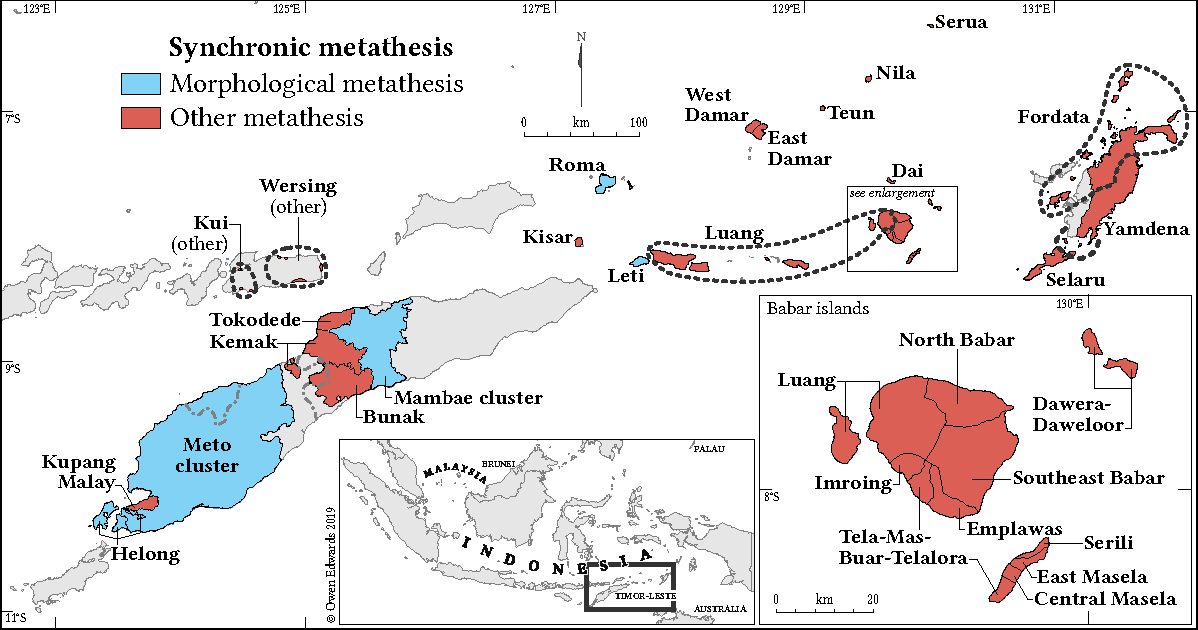
\includegraphics[width=\columnwidth]{SynchronicMetathesis.pdf}
\end{figure}

A map of languages in the greater Timor region
with synchronic metathesis is given in \frf{fig:CVMetTimReg},
based on \citet[135ff]{sc15}, a survey of the literature,
and my own fieldwork.
This map further marks languages in which metathesis
is known to be morphological in at least some environments.
\emph{Other metathesis} in \frf{fig:CVMetTimReg} is used for languages
with phonologically or morphemically conditioned metathesis,
as well as for languages for which too little data is available
to determine the nature of their metathesis.

There are at least five languages of the greater Timor region
with morphological metathesis in at least some environments:
Leti (\srf{sec:Let}), Roma (\srf{sec:Rom}), Mambae (\srf{sec:Mam}),
Helong (\srf{sec:Hel}) and the Meto cluster (of which Amarasi is a member).
A further twenty or so languages have synchronic
metathesis which is phonologically conditioned,
morphemically conditioned or not yet unambiguously established as morphological.

I begin my discussion with Kwara'ae (\srf{sec:Kwa})
and Rotuman (\srf{sec:Rot}), both of which are spoken in the Pacific
and outside the greater Timor region.
I then discuss cases of synchronic metathesis
in the greater Timor region starting with the non-Austronesian
languages Wersing (\srf{sec:Wer}) and Bunak (\srf{sec:Bun}).
After this I discuss synchronic metathesis among Austronesian
languages of the greater Timor region moving geographically
closer to Meto with each language discussed.

Before proceeding with the discussion
it is necessary to clarify two points.
Firstly, in some cases I give isolated examples of metathesis
of the type X {\ra} Y
(e.g. Rotuman \it{ho\tbr{sa}} {\ra} \it{ho\tbr{as}}
`flower' on page \pageref{ex:VCV->VVC})
or X + Z {\ra} YZ (e.g. Luang \it{ʔer\tbr{nu}} + \it{la}
{\ra} \it{ʔer\tbr{un}la} `go down to' on page \pageref{ex:LuaMet}).
In all such cases the form before the arrow is
a form which surfaces in certain contexts.
Thus, all putative examples of metathesis throughout this section
are based on true surface alternations.\footnote{
		Readers who find a particular analysis involving metathesis
		unconvincing should consult the original sources for full
		discussion and justification.}

Secondly, in such examples the form
before the arrow is the presumed underlying form.
The identification of underlying forms follows that of the sources,
which in turn is usually based on phonological and morphological analysis.
However, I do not usually repeat here the evidence for this analysis.
Interested readers should consult the original sources.
Again, in all cases the presumed underlying form
is a form which surfaces in certain contexts, as discussed above.
	\subsection{Kwara'ae}\label{sec:Kwa}
Metathesis in Kwara'ae has been described by
\citet{so80} and \citet{he04,he05}.
\citet{blga98} also present previously unpublished data
collected by Andrew Pawley and David Gegeo.
Metathesis in Kwara'ae has been analysed as phonologically conditioned (\srf{sec:PhoMet})
but it is not restricted to a subset of words with specific phonological properties.
Instead nearly every word of the lexicon is affected by metathesis in Kwara'ae.

\subsubsection{Forms}
Metathesis in Kwara'ae is CV {\ra} VC metathesis.
Examples are shown in \qf{ex:KwVCV->VVC} below.
In the literature on Kwara'ae the unmetathesised
form (U\=/form) is called the \emph{citation form} and the metathesised form
(M\=/form) is called the \emph{normal form}.
I refer to them with the more iconic terms \emph{U\=/form} and \emph{M\=/form}.

\begin{exe}
	\ex{V\sub{1}CV\sub{2} {\ra} V\sub{1}V\sub{2}C \hfill\citep[1]{he04}}\label{ex:KwVCV->VVC}
	\sn{\gw\begin{tabular}{rcll}
		 U\=/form 					&			& \mc{2}{l}{M\=/form}  \\
		\it{ˈlo.\tbr{ʔi}} &{\ra}& \it{ˈlo\tbr{i̯ʔ}} & `snake' \\
		\it{ˈbu.\tbr{ri}} &{\ra}& \it{ˈbu̯\tbr{ir}} & `behind' \\
		\it{ˈbo.\tbr{re}} &{\ra}& \it{ˈbo̯\tbr{er}} & `although' \\
	\end{tabular}}
\end{exe}

Depending on the length of the word,
metathesis in Kwara'ae can occur multiple times.
Two examples are given in \qf{ex:MulMetKwa} below.
The difference in stress which is seen in examples such as
\it{da.ˈro.ʔa.ˌni.da} {\ra} \it{ˈdao̯r.ʔa.ˌni̯ɛd} `to share them'
is significant and is the phonological conditioning environment
by which \cite{he04} analyses Kwara'ae metathesis.

\begin{exe}
	\ex{Kwara'ae multiple metatheses: \hfill\citep[2]{he04}}\label{ex:MulMetKwa}
	\sn{\gw\begin{tabular}{rcll}
		 U\=/form														&			& M\=/form &  \\
		\it{ˈke.\tbr{ta}.ˌla.\tbr{ku}} 	&{\ra}& \it{ˈke̯\tbr{at}.ˌla\tbr{u̯k}} & `my height' \\
		\it{da.ˈ\tbr{ro}.ʔa.ˌni.\tbr{da}}&{\ra}& \it{ˈda\tbr{o̯r}.ʔa.ˌni̯\tbr{ɛd}} & `to share them' \\
	\end{tabular}}
\end{exe}

Metathesis in Kwara'ae often triggers other phonological processes
including glide formation, vowel deletion, and umlaut.
The different phonological processes with which metathesis
is associated are described in \srf{sec:KwaGliFor}--\srf{sec:KwaSum} below.

Published descriptions of Kwara'ae report different
details for some of these phonological processes.
In part these differences may stem from researchers working
with different speakers of different ages.
However, another likely source of variation
is that a single speaker can also use
different M\=/forms depending on speech speed
(Patrick Andrews p.c. February 2015).

In addition to the difference in metathesis,
U\=/forms have the labiodental fricative [f]
where M\=/forms have the voiceless glottal fricative [h] \citep[18]{he04}.

\paragraph{Glide formation}\label{sec:KwaGliFor}
As can be seen from the examples in \qf{ex:KwVCV->VVC} and \qf{ex:MulMetKwa},
when a vowel sequence surfaces in the M\=/form,
the higher vowel is realised as a glide. %\citep[22]{he04}.
If the vowels are of equal height,
as in \it{ˈbo.re} {\ra} \it{ˈbo̯er} `although',
the first vowel is realised as a glide.
\citet[319]{so80} likewise states that metathesised forms consist only of one syllable,
though he does not give rules for which of the underlying vowels surfaces as a glide.

When a word ends in a vowel sequence,
the M\=/form is derived from the U\=/form through glide formation alone.
This is shown in \qf{KwaVV} below:

\begin{exe}
\ex{V\sub{1}V\sub{2} {\ra} V̯\sub{1}V\sub{2}\hfill\citep[13]{he04}}\label{KwaVV}
	\sn{\gw\begin{tabular}{rcll}
		 U\=/form								&			& M\=/form &  \\
		\it{ʔo.ˈd\tbr{o.a}} 	&{\ra}& \it{ˈʔo.d\tbr{o̯a}} & `wall' \\
		\it{ˈd\tbr{o.e}} 			&{\ra}& \it{ˈd\tbr{o̯e}} & `great, big' \\
		\it{ˈne.i.ˌr\tbr{i.a}}&{\ra}& \it{ˈnei̯.ˌr\tbr{i̯ɛ}} & `this one' \\
	\end{tabular}}%
\end{exe}

\paragraph{Vowel deletion}
When a word ends in V\sub{1}V\sub{2}CV\sub{3}{\#},
and V\sub{2} and V\sub{3} are of the same quality,
the first two vowels undergo glide formation and
the final vowel is deleted.
This is shown in \qf{KwaVseq1} below.

\begin{exe}
	\ex{V\sub{1}{\sub{α}}V\sub{2}{\sub{β}}CV\sub{3}{\sub{β}} {\ra} V̯\sub{1}{\sub{α}}V\sub{2}{\sub{β}}C \hfill\citep[27-28]{he04}}\label{KwaVseq1}
	\sn{\gw\begin{tabular}{rcll}
			U\=/form							&			& M\=/form &  \\
			\it{fu.ˈi.r\tbr{i}} &{\ra}& \it{ˈhu̯ir} & `that' \\
			\it{bi.ˈa.l\tbr{a}} &{\ra}& \it{ˈbi̯al} & `smoke' \\
	\end{tabular}}%
\end{exe}

\paragraph{Vowel shift}\label{sec:KwaVoShi}
The low central vowel /a/ has a different quality
after metathesis when the preceding vowel is high.
It is described as schwa [ə] by \citet[315]{so80},
while \citet[23]{he04} describes it as varying between
[ɛ] and [ə] after /i/ and as [ʌ] after /u/.
Examples are given in \qf{Kw2} below.

\begin{exe}
	\ex{V\tsc{[+hi]}Ca {\ra} V̯əC: \hfill\citep[23]{he04}}\label{Kw2}
		\sn{\gw\begin{tabular}{rcll}
			 	U\=/form								&			& M\=/form &  \\
				\it{a.ˈsi.\tbr{la}} 	&{\ra}& \it{ˈa.ˌsi̯\tbr{ɛl} {\tl} ˈa.ˌsi̯\tbr{əl}} & `sweet' \\
				\it{fa.ˈʔu.\tbr{ta}}	&{\ra}& \it{ˈha.ˌʔu̯\tbr{ʌt}} & `which, how, why' \\
		\end{tabular}}
\end{exe}

Likewise, certain combinations of vowel ``fuse'' into
a single vowel rather than a sequence of glide and vowel.
\citet[316]{so80} gives a rule in which /oi/ is realised as [øˑ],
/oe/ as [œˑ], /ae/ as [æˑ] and /ai/ is realised as either [ɛi] or [ɛˑ].
This is similar to the processes of umlaut which have
operated in the Germanic languages (\srf{sec:OriUml}).


\begin{exe}
	\ex{V\sub{α}CV\sub{β} {\ra} V\sub{αβ}C \hfill\citep[316]{so80}}\label{KwVfusionS}
		\sn{\gw\begin{tabular}{rcll}
			 U\=/form														&			& M\=/form &  \\
			\it{m\tbr{o}l\tbr{i}} 						&{\ra}& \it{m\tbr{øˑ}l} 							& `lemon' \\
			\it{as\tbr{o}f\tbr{e}} 						&{\ra}& \it{as\tbr{œˑ}f} 						& `rat' \\
			\it{m\tbr{a}ʔ\tbr{e}t\tbr{a}ʔ\tbr{e}elo}&{\ra}& \it{m\tbr{æˑ}ʔ.t\tbr{æˑ}ʔ.eol} & `doorway' \\
			\it{d\tbr{a}m\tbr{i}} 						&{\ra}& \it{d\tbr{ɛi}m {\tl} d\tbr{ɛˑ}m}	& `gum' \\
		\end{tabular}}
\end{exe}

\citet{he04} does not report front rounded vowels,
but he does report a similar process when the first vowel of the sequence is /a/.
He states that ``[{\ldots}] there is some free variation: if V\sub{2} = [e], [i] or [u],
sometimes the vowel combination can be realized as a single vowel.''
He only gives examples of /ae/ {\ra} [æˑ], /ai/ {\ra} [eˑ] and /au/ {\ra} [oˑ].

\begin{exe}
	\ex{V\sub{α}CV\sub{β} {\ra} V\sub{αβ}C \hfill\citep[24]{he04}}\label{KwVfusionH}
		\sn{\gw\begin{tabular}{rcll}
			 U\=/form										&			& M\=/form &  \\
			\it{ˈs\tbr{a}.t\tbr{e}}		&{\ra}& \it{ˈs\tbr{æ}ˑt} {\tl} \it{ˈs\tbr{ae̯}t} & `chin, beard' \\
			\it{ˈm\tbr{a}.ʔ\tbr{i}}		&{\ra}& \it{ˈm\tbr{eˑ}ʔ} {\tl} \it{ˈm\tbr{ai̯}ʔ} & `come' \\
			\it{li.ˈm\tbr{a}.k\tbr{u}}&{\ra}& \it{ˈli.ˌm\tbr{oˑ}k} {\tl} \it{ˈli.m\tbr{au̯}k} & `my hand' \\
		\end{tabular}}%
\end{exe}

\paragraph{Long vowels}\label{sec:KwaLonVow}
When the penultimate and final vowel of the U\=/form are identical,
\citet{so80}, Pawley and Gegeo (cited in \citealt{blga98}) and \citet{he04}
all transcribe the vowel of the M\=/form as half-long, using the symbol [ˑ].
Other descriptions of Kwara'ae, such as,
\citet{si77} and \citet{trha83} do not transcribe such vowels as long.

\begin{exe}
	\ex{V\sub{α}CV\sub{α} {\ra} V\sub{α}ˑC \hfill\citep[25]{he04}}\label{KwlongV}
		\sn{\gw\begin{tabular}{rcll}
			 U\=/form									&			& M\=/form &  \\
			\it{ˈk\tbr{i}.n\tbr{i}} &{\ra}& \it{ˈk\tbr{iˑ}n} & `female' \\
			\it{ˈm\tbr{a}.n\tbr{a}} &{\ra}& \it{ˈm\tbr{aˑ}n} & `her/his eye' \\
			\it{ˈm\tbr{o}.k\tbr{o}} &{\ra}& \it{ˈm\tbr{ɔˑ}k} & `smell' \\
		\end{tabular}}
\end{exe}

However, as noted by \citet[25]{he04},
no author justifies the use of this half-long mark,
with \citeauthor{he04} indicating that this is a point for further research.
An instrumental phonetic study of Kwara'ae vowels
would probably settle the matter.\footnote{
		For Amarasi I carried out an instrumental study of vowel length
		in which I showed that there is a statistically significant
		difference in length between the penultimate vowel of a U\=/form
		with identical penultimate and final vowels and the final
		vowel of the M\=/form of such words.
		I analyse this difference in length as being due to the M\=/forms
		containing a sequence of two identical vowels.
		(see \srf{sec:QuaLenVowSeq} and \srf{sec:QuaMfoEndVVC}).}
It is also possible that such vowels are long in some contexts and short in others,
depending on variables such as phrasal stress and the rate of speech.

\paragraph{Voiceless vowels}\label{sec:KwaVoiVow}
Optional voiceless vowels also occur after certain consonants in the U\=/form.
\citet[19]{he04} reports such vowels after the consonants [ʔ], [h], [l] and [s].
These vowels do not count as vowels for the purposes of stress assignment,
with stress falling on the penultimate vowel, not counting final voiceless vowels.
After word-final stops, voiceless vowels do not occur,
though the final stop is often strongly aspirated.

\begin{exe}
	\ex{V\sub{1}CV\sub{2} {\ra} V\sub{1}V\sub{2}C{\r*V}\sub{2} \hfill\citep[19]{he04}}\label{KwvoicelessVH}
		\sn{\gw\begin{tabular}{rcll}
			 U\=/form			&			& M\=/form &  \\
			\it{ˈma.ʔu} &{\ra}& \it{ˈmau̯ʔ\tbr{u̥}} & `fear' \\
			\it{ˈʔa.fe} &{\ra}& \it{ˈʔae̯h\tbr{e̥}} & `wife' \\
			\it{ˈbu.su} &{\ra}& \it{ˈbuˑs\tbr{u̥}} & `to burst' \\
			\it{ˈro.do} &{\ra}& \it{ˈrɔˑ\tbr{dʰ}} & `night' \\
			\it{ˈnau̯.ku} &{\ra}& \it{ˈnau̯\tbr{kʰ}} & `I' \\
		\end{tabular}}
\end{exe}

Pawley and Gegeo (cited in \citealt{blga98})
describe voiceless vowels in a wider variety of contexts than is described by \citet{he04}.
According to Pawley and Gegeo, a final voiceless vowel is the usual realisation of words in the M\=/form.
Such vowels only do not occur when there is a word-final nasal
or if the resulting diphthong is a sequence of a high vowel followed by a non-high vowel.

\begin{exe}
	\ex{V\sub{1}CV\sub{2} {\ra} V\sub{1}V\sub{2}C{V̥}\sub{2} \hfill(Pawley and Gegeo in \citealt[530]{blga98})}\label{KwvoicelessVBG}
		\sn{\gw\begin{tabular}{rcll}
			 U\=/form			&			& M\=/form &  \\
			\it{ˈfusi}	&{\ra}& \it{huis\tbr{i̥}} & `cat' \\
			\it{ˈkado}	&{\ra}& \it{kaod\tbr{o̥}} & `thin' \\
			\it{ˈoso}		&{\ra}& \it{oˑs\tbr{o̥}} & `lie' \\
	\end{tabular}}
\end{exe}

According to \citet[20]{he04},
the differences between his data and the data cited by \citet{blga98}
likely comes from working with speakers of different generations.
\citeauthor{he04} states: \emph``[{\ldots}] it's reasonable that her [Kwara'ae consultant's]
speech pattern reflects another stage in the decline of the final vowel.''
%The aspiration of final stops reported by \citet[18]{he04} seems also to
%represent the final remnant of the voiceless vowels reported by Pawley and Gegeo.

\begin{table}[h]
	\caption{Kwara'ae metathesis}\label{tab:KwaMet}
	\begin{tabular}{c|ccccccl}
		\lsptoprule
	V\sub{1}{\da}	&i							&e						&a				&o	&u			&	{\la}V\sub{2}\\			
			\midrule
			i	&{iˑ}										&--						&jɛ, jə		&jo	&ju			&\\
			e	&{ej}										&ɛˑ						&e̯a				&e̯o	&ew			&\\
			a	&{aj, ej, eˑ, (ɛj, ɛˑ)}	&{æ;, ae̯}			&aˑ				&ao̯	&aw, oˑ	&\\
			o	&{oj, (øˑ)}							&o̯e, we, (œˑ)	&o̯a				&ɔˑ	&ow			&\\
			u	&{wi}										&wɛ						&wʌ, (wə)	&--	&uˑ			&\\
		\lspbottomrule
	\end{tabular}
\end{table}

\paragraph{Summary}\label{sec:KwaSum}
The processes with which metathesis in Kwara'ae is associated
include glide formation, umlaut, and vowel deletion.
The effects of deriving the M\=/form on the first
and second vowels of the U\=/form in Kwara'ae are given in \trf{tab:KwaMet}.
This table is adapted from \citep[26]{he04} with qualities reported by \citet{so80} included in brackets.
The symbols used by \citeauthor{he04} for the high vowel glides:
[u̯] and [i̯], have been replaced with the symbols [w] and [j].

\subsubsection{Distribution of metathesis}\label{sec:KwaFun}
U\=/forms and M\=/forms in Kwara'ae belong to different speech registers.
In everyday normal speech the M\=/form is used,
while the U\=/form is used in traditional songs,
for clarification \citep[3]{he04}, and when calling out.
\citet[19]{wage86} report that calling out has three main uses in Kwara'ae discourse:

\begin{quote}
First, people call out for practical reasons in running a household,
such as to locate a missing person or to bring a family member home for a meal.
Secondly, a Kwara'ae man or woman working in the bush and hearing someone
working nearby but out of sight will call out to seek identification of the other person.
Thirdly, people call out from house to house, or as someone passes on the path, as a strictly social activity.
They ask polite questions, or joke, tease, and engage in pleasant banter. \hfill\citep{wage86}
\end{quote}

In addition to the use of unmetathesised forms, calling out is marked
by a special intonation contour and certain emphatic particles.
Two examples of Kwara'ae calling out are given in \qf{KwCallingOut} below.
Note also the extra length on the final syllable of the second form of `father' in example
\qf{KwCallingOut1} as well as the particle \emph{ku} in \qf{KwCallingOut2}.
These two features are also distinctive of calling out.

\begin{exe}\let\eachwordone=\itshape
	\ex{Kwara'ae calling out: \hfill\citep[24,21]{wage86}}\label{KwCallingOut}
		\begin{xlist}
			\ex{
				\gll maʔ! ma\tbr{ʔaːː}! \\
				father{\textbackslash}\tsc{m} father{\tbrU} \\
				\glt `Dad! Da-ad!'\label{KwCallingOut1}}
			\ex{
				\gll Sa\tbr{la}! Sal! Sal ku! lae maiʔ tua hain Mo\tbr{sa}! \\
				Sala{\tbrU} Sala{\M} Sala{\M} \tsc{part} go here stay with:\tsc{3sg.poss} Mosa{\tbrU} \\
				\glt `Sala! Sala! Hey, Sala! Come here and babysit Mosa!' \label{KwCallingOut2}}
		\end{xlist}
\end{exe}

The use of different forms in different speech registers is confirmed by Patrick Andrews
(p.c. February 2015)
who reports that (among other uses) the unmetathesised forms
are used when making a point to a child or to emphasise words in a speech.
He compares the use of the metathesised forms to that of English contractions,
such as \it{couldn't} from \it{could not},
with the former being the everyday form and the latter being used in special circumstances.
This difference in distribution suggests that different forms
are used in different (discourse) pragmatic contexts.

\cite{he04} proposes an analysis of Kwara'ae metathesis framed within Optimality Theory
in which metathesis is conditioned by stress.
Under this analysis, metathesis in Kwara'ae is a response
to the need to make stressed syllables heavy,
with a vowel-glide combination counting as a heavy syllable.
This analysis is discussed in more detail in \srf{sec:ProMorKwa}.

Given that different forms are used in different speech registers,
an analysis of Kwara'ae metathesis as being driven by stress
would predict that different registers have different stress rules.
While it is likely that such a hypothesis would be borne out,
to the best of my knowledge this has not yet been demonstrated.

Nearly every word in Kwara'ae is affected by metathesis.
If it is the case that different speech registers have
different stress patterns, which in turn drives the metathesis,
Kwara'ae has (rampant) phonologically conditioned metathesis
though the phonological conditions triggering metathesis
are themselves driven by the discourse.

	\subsection{Rotuman}\label{sec:Rot}
\il{Rotuman|(}Rotuman has perhaps the most famous case of morphological metathesis.
Rotuman is an Austronesian Oceanic language spoken on Rotuma island
in the Pacific Ocean located about 480 kilometres north of the main islands of Fiji.
Metathesis occurs in multiple environments in Rotuman,
discussed in fuller detail in \srf{sec:RotFun}
In some cases metathesis is phonologically conditioned (\srf{sec:PhoMet}),
in some cases it is morphemically conditioned (\srf{sec:MorpheConMet}),
and in some cases it is morphological (\srf{sec:MorMet}).

Rotuman was first described by \citet{ch40} which is a grammar and dictionary of the language.
\citeauthor{ch39} also published several Rotuman texts between 1937--39 in the journal \it{Oceania}
which were reprinted in one volume as \citet{ch39}.
Both \citet{be87} and \citet{va02} also present descriptions of
Rotuman based on their own fieldwork.
Each of these descriptions differs in details.
This may be partly because the authors worked with different
speakers at different times and may also be partly because they use
different terminology to describe the same phenomena.

\subsubsection{Forms}\label{sec:RotFor}
Each word in Rotuman has two forms, which I call the the U-form and M-form.
The traditional names coined by \cite{ch40} are the \it{complete phase} for the U-form
and the \it{incomplete phase} for the M-form.
The U-form is historically more conservative than the M-form.

\cite{ch40} identifies four phonological processes
which derive the M-form from the U-form.
These processes are vowel deletion (a.k.a apocope, truncation or subtraction),
umlaut, metathesis and vowel shortening.
There are also words which do not have two distinct forms.
Which process applies depends on the phonological shape of the U-form.
%Examples are given in \qf{ex:RotLonShoChu} below,
%and discussed in more detail in \srf{sec:RotDip}--\srf{sec:RotSum}.

%\begin{exe}
%	\ex{Rotuman U-forms and M-forms \hfill\citep[85]{ch40}}\label{ex:RotLonShoChu}
%		\sn{\begin{tabular}{llll}
%			U-form&M-form	&						&Process \\
%			\it{mata}	&\it{mat}			&`wet'			&apocope \\
%			\it{mose}	&\it{mœs}			&`to sleep'	&umlaut	\\
%			\it{toka}	&\it{toak}		&`to cease'	&metathesis\\
%			\it{ʧao}	&\it{ʧ\u{a}o}	&`spear'		&V shortening \\
%			\it{rii}	&\it{rii}			&`house'		&n./a. \\
%		\end{tabular}}
%\end{exe}

\paragraph{Vowel shortening/diphthongisation}\label{sec:RotDip}
For words which end in a sequence of non-identical vowels,
\cite[85]{ch40} describes the M-form as being formed
by shortening the initial vowel of the sequence.
Examples are given in \qf{VV->VV-Chu} below.

\begin{exe}
	\ex{Rotuman V{\sub{α}}V{\sub{β}} {\ra} \u{V}{\sub{α}}V{\sub{β}} \hfill\citep[85]{ch40}}\label{VV->VV-Chu}
	\sn{\gw\begin{tabular}{lcll}
			U-form		&		&M-form			&\\
		\it{pupui}	&\ra& \it{pup\u{u}i}	& `floor' \\
		\it{ʔesʔao} &\ra& \it{ʔesʔ\u{a}o} & `useful' \\
		\it{lelei}	&\ra& \it{lel\u{e}i}	& `good' \\
		\it{foʔou}	&\ra& \it{foʔ\u{o}u}	& `new' \\
	\end{tabular}}
\end{exe}

\cite{va02} describes a process of diphthongisation
in which the less sonorous vowel becomes a glide.
This glide formation may be either a further development 
of \citeauthor{ch40}'s shortened vowels, or it may that
a single phenomenon was perceived and described differently
by each of these authors.

\begin{exe}
	\ex{Rotuman V{\sub{α}}V{\sub{β}} {\ra} V̯{\sub{α}}V{\sub{β}} {\tl} V{\sub{α}}V̯{\sub{β}}
	\hfill\citet[4,7--9]{va02}}\label{VV->VV-Vam}
		\sn{\gw\begin{tabular}{lcll}
			U-form			&		&	M-form		&\\
			\it{lio}		&\ra& \it{ljo}	& `voice' \\
			\it{fau}		&\ra& \it{faw}	& `year' \\
			\it{fui}		&\ra& \it{fuj}	& `piece of garland' \\
			\it{fɒi}		&\ra& \it{fɒj}	& `chop down' \\
			\it{momoe}	&\ra& \it{momoe̯} & `k.o. tree' \\
		\end{tabular}}
\end{exe}

According to \citet[210]{be87} the vowel sequences which
diphthongise are those in which the second vowel is /a/
as well as sequences of a high vowel followed by /o/.
\citeauthor{be87} also reports that /a/
is realised as [ɔ] after a glide derived
from one of the high-front vowels.

\begin{exe}
	\ex{Rotuman V{\sub{α}}V{\sub{β}} {\ra} V̯{\sub{α}}V{\sub{β}} \hfill\citep[210]{be87}}\label{RotDip-be}
	\sn{\gw\begin{tabular}{lcll}
			U-form	&		&	M-form		&\\
		\it{ʔea}	&\ra& \it{ʔja}	& `to say' \\
		\it{foa}	&\ra& \it{fwa}	& `coconut scraper' \\
		\it{kia}	&\ra& \it{kjɔ}	& `neck' \\
		\it{sua}	&\ra& \it{swɔ}	& `shoot (of a plant)' \\
	\end{tabular}}
\end{exe}

\paragraph{Metathesis}\label{sec:RotMet}
When the U-form ends in VCV and the penultimate vowel is higher than the final vowel,
the M-form is derived by final consonant-vowel metathesis.
Examples are given in \qf{ex:VCV->VVC} below.

\begin{exe}
	\ex{Rotuman V\sub{1}CV\sub{2} {\ra} V\sub{1}V\sub{2}C \hfill\citep[14]{ch40}}\label{ex:VCV->VVC}
		\sn{\gw\begin{tabular}{lcll}
			U-form					&		&M-form&\\
			\it{pu\tbr{re}} &\ra& \it{pu\tbr{er}} & `to rule, decide' \\
			\it{ho\tbr{sa}} &\ra& \it{ho\tbr{as}} & `flower' \\
			\it{ti\tbr{ko}} &\ra& \it{ti\tbr{ok}} & `flesh' \\
			\it{pe\tbr{pa}} &\ra& \it{pe\tbr{ap}} & `paper' \\
		\end{tabular}}
\end{exe}

Both \citet{va02} and \citet{be87} report that after metathesis
the penultimate vowel becomes a glide;
/u/ and /o/ become [w] while /i/ and /e/ become [j].
Examples are given in \qf{ex:VCV->VVC-Vam} below.

\begin{exe}
	\ex{Rotuman V\sub{1}CV\sub{2} {\ra} V̯\sub{1}V\sub{2}C \hfill\citep[3]{va02}}\label{ex:VCV->VVC-Vam}
	\sn{\gw\begin{tabular}{lcll}
			U-form				&		&	M-form&\\
		\it{pu\tbr{re}} &\ra& \it{pw\tbr{ɛr}} & `rule' \\
		\it{fu\tbr{pa}} &\ra& \it{fw\tbr{ap}} & `to distribute' \\
		\it{ʔi\tbr{ko}} &\ra& \it{ʔj\tbr{ɔk}} & `thrust' \\
	\end{tabular}}
\end{exe}

\citet[208]{be87} reports that when the penultimate vowel is a high vowel,
the final vowel becomes [ɔ] after metathesis.
Otherwise, the final vowel retains its original quality.
Examples are given in \qf{ex:VCV->VVC-Bes} below.

\begin{exe}
	\ex{Rotuman V\sub{1}CV\sub{2} {\ra} V̯\sub{1}V\sub{2}C \hfill\citep[208]{be87}}\label{ex:VCV->VVC-Bes}
	\sn{\gw\begin{tabular}{lcll}
			U-form				&		&	M-form&\\
		\it{ti\tbr{fe}}	&\ra& \it{tj\tbr{ɔf}} & `pearl shell' \\
		\it{pi\tbr{ʧa}} &\ra& \it{pj\tbr{ɔʧ}} & `rat' \\
		\it{hu\tbr{ŋe}}	&\ra& \it{hw\tbr{ɔŋ}} & `to breathe' \\
		\it{pu\tbr{ka}}	&\ra& \it{pw\tbr{ɔk}} & `k.o. creeper' \\
		\it{he\tbr{pa}}	&\ra& \it{hj\tbr{ap}} & `broad' \\
		\it{lo\tbr{ŋa}}	&\ra& \it{lw\tbr{aŋ}} & `towards the interior of the island' \\
	\end{tabular}}
\end{exe}

It is not entirely clear whether the diphthongisation
after metathesis reported by \cite{be87} and \cite{va02}
is a recent development or whether it was also present
while \citeauthor{ch40} worked on Rotuman.

On the one hand, it is clear from the detailed account of
Rotuman phonetics given by \citet[64--84]{ch40},
that he was an excellent phonetician.
Given his identification of shortened vowels
in the derivation of M-forms (\srf{sec:RotDip}),
it seems likely that if diphthongisation (or shortened vowels)
were present after metathesis he would have reported it.

On the other hand, \citet[86]{ch40} states
``[T]he stress seems to be levelled out, so
to speak, in the inc[omplete] phase.
Thus: \it{fo}ra becomes \it{foar}, which is pronounced almost,
though perhaps not quite, as one syllable,
the stress being evenly distributed [\ldots]''
This statement perhaps indicates that diphthongisation
was an optional feature of Rotuman metathesised
forms in \citeauthor{ch40}'s day.

\paragraph{Umlaut}\label{sec:RotUml}
When the penultimate vowel is a back vowel and the final vowel a front vowel,
the M-form is derived via umlaut of the penultimate vowel
so long as this vowel is not higher than the final vowel.

\citet[79]{ch40} reports that /u/ becomes [y],
/o/ becomes [œ] when the final vowel is /e/,
and that /o/ becomes [ø] when the final vowel is /i/.\footnote{
	\cite{ch40} describes the vowel in the M-form of oCe{\#} final words
	(e.g. \it{mose} {\ra} \it{mœs} `sleep')
	as ``[\ldots] similar to the wider German \it{ö}, as in \it{gespött},
	and to the sound of \it{eu} in the French \it{jeune}.''
	He contrasts `normal \it{ö}' (which ``[\ldots] arises in place of normal \it{o} when a following \it{e} is elided'')
	with so-called `narrow \it{ö}' (arising ``[\ldots] in place of narrow \it{o} when a following \it{i} is elided'')
	which is described as ``[\ldots] similar to the narrower German \it{ö}, as in \it{schön},
	and to the sound of \it{eu} in the French \it{peu}.''
	I interpret `normal \it{ö}' as a mid-low front-rounded vowel [œ]
	and `narrow \it{ö}' as a mid-high front-rounded vowel [ø].}
He also transcribes the outcome of umlauted /ɒ/ as \it{<\.a>},
describing it as ``[\ldots] a little wider [lower] than \it{a} in `cat' [\ldots]
but differs from it in containing just a suggestion of the sound of \it{u} in `cut' or `but.'{''}
In interpret \citeauthor{ch40}'s \it{<\.a>} as a low front rounded vowel [ɶ].

Examples of Rotuman umlaut are given in \qf{RotUml-ch} below,
which also gives hypothetical intermediate forms
showing the way such umlaut probably developed from metathesis.
In Kwara'ae (\srf{sec:KwaVoShi}) words containing some of the vowel combinations
shown in \qf{RotUml-ch} have M-forms which vary between displaying metathesis and umlaut.

\begin{exe}
\ex{V\tsc{[+rnd]}CV\tsc{[+fr]} {\ra} V\tsc{[+rnd,+fr]}C \hfill\citep[79-80]{ch40}}\label{RotUml-ch}
	\sn{\gw\begin{tabular}{lclcll}
			U-form	& &						& &	M-form&\\
		\it{ʔuli} &>&\it{*ʔuil}	&>& \it{ʔyl} & `skin' \\
		\it{mori} &>&\it{*moir}	&>& \it{mør} & `orange (fruit)'	 \\
		\it{mose} &>&\it{*moes}	&>& \it{mœs} & `to sleep' \\
		\it{ʔɒfi} &>&\it{*ʔɒif}	&>& \it{ʔɶf} & `to bite' \\
	\end{tabular}}
\end{exe}

\citet{va02} reports that /o/ becomes [ø] under umlaut,
/u/ becomes [y] and /ɒ/ becomes the lower mid-front-rounded [œ].
Examples are given in \qf{RotUml-va}

\begin{exe}
\ex{Rotuman V\tsc{[+ba]}CV\tsc{[+fr]} {\ra} V\tsc{[+fr]}C \hfill\citep[3]{va02}}\label{RotUml-va}
	\sn{\gw\begin{tabular}{lcll}
			U-form	&		&	M-form&\\
		\it{futi} &\ra& \it{fyt} & `to pull' \\
		\it{mose} &\ra& \it{møs} & `to sleep' \\
		\it{pɒri} &\ra& \it{pœri} & `banana' \\
	\end{tabular}}
\end{exe}

\citeauthor{be87}'s data agrees with \citeauthor{va02} on the outcome of /o/ and /u/,
though he reports that /ɔ/ (equivalent to \citeauthor{ch40}'s and \citeauthor{va02}'s /ɒ/)
becomes either [ɛ] or [æ] in free variation in certain words.
Examples are given in \qf{RotUml-be} below.

\begin{exe}
\ex{Rotuman V\tsc{[+ba]}CV\tsc{[+fr]} {\ra} V\tsc{[+fr]}C \hfill\citep[209]{be87}}\label{RotUml-be}
	\sn{\gw\begin{tabular}{lcll}
			U-form	&		&	M-form&\\
		\it{pɔti} &\ra& \it{pɛt} & `scar' \\
		\it{hɔʔi} &\ra& \it{hɛʔ} & `to pull' \\
		\it{pɔni} &\ra& \it{pɛn} & `paint' \\
	\end{tabular}}
\end{exe}

All authors agree that umlaut of /u/ or /o/ spreads leftwards to identical vowels.
Examples are given in \qf{RotUmlSpr} below

\begin{exe}
\ex{Rotuman umlaut spreading: \hfill\citep[79f]{ch40}}\label{RotUmlSpr}
	\sn{\gw\begin{tabular}{lcll}
			U-form			&\ra&	M-form&\\
		\it{furfuruki}&\ra& \it{fyrfyryk} & `pimple' \\
		\it{roromi} 	&\ra& \it{rørøm} & `unexpectedly' \\
		\it{popore} 	&\ra& \it{pœpœr} & `to dash, dart' \\
	\end{tabular}}%
\end{exe}

\paragraph{Apocope}\label{sec:RotApo}
In all situations not covered by diphthongisation, metathesis or umlaut,
the M-form is derived by deleting the final vowel of the U-form.
This includes when each vowel is identical and
when the penultimate vowel is lower than a final back vowel.
Examples are shown in \qf{ex:VCV->VC} below.

\begin{exe}
	\ex{Rotuman VCV {\ra} VC \hfill\citep[13]{ch40}}\label{ex:VCV->VC}
	\sn{\gw\begin{tabular}{lcll}
			U-form		&		&	M-form			&\\
		\it{haŋa}		&\ra& \it{haŋ}		& `to feed' \\
		\it{hɒŋu}		&\ra& \it{hɒŋ}		& `to awaken' \\
		\it{læʧe}	&\ra& \it{læʧ}		& `coral' \\
		\it{tokiri} &\ra& \it{tokir}	& `to roll' \\
		\it{hoto} 	&\ra& \it{hot}		& `to jump' \\
		\it{heleʔu} &\ra& \it{heleʔ}	& `to arrive' \\
	\end{tabular}}
\end{exe}

The lack of overt metathesis in such examples is comparable
to the Amarasi data in which words with a certain phonotactic
shape form their M-form by surface vowel deletion and/or consonant deletion (Chapter \ref{ch:StrMetAma}).

\paragraph{No change}
Words ending in two identical vowels
do not usually have distinct U-forms and M-forms according to \citet[85]{ch40},
except before certain suffixes in which case the final vowel of U-form is lengthened.
Examples are given in \qf{ex:VV->VV} below.

\begin{exe}
	\ex{Rotuman V{\sub{α}}V{\sub{α}} {\ra} V{\sub{α}}V{\sub{α}} \hfill\citep[85]{ch40}}\label{ex:VV->VV}
	\sn{\gw\begin{tabular}{lcll}
			U-form	&		&	M-form&\\
		\it{rii}	&\ra& \it{rii}	& `house' \\
		\it{ree}	&\ra& \it{ree}	& `to do' \\
%		\it{reeː-} & \it{ree-}	& `to do' \\
	\end{tabular}}
\end{exe}

\citet{be87} reports that when the sequence of two identical vowels is /aa/,
the M-form is formed by deleting the final vowel.
In other situations \citeauthor{be87} reports no difference in the two forms.
Examples are given in \qf{ex:aa->a} below.

\begin{exe}
	\ex{Rotuman /aa/ {\ra} /a/ \hfill\citep[212]{be87}}\label{ex:aa->a}
	\sn{\gw\begin{tabular}{lcll}
		 U-form		&		&	M-form&\\
		\it{ʔaa}	&\ra& \it{ʔa} & `bite' \\
		\it{ree}	&\ra& \it{ree} & `do' \\
		\it{luu}	&\ra& \it{luu} & `rope' \\
	\end{tabular}}%
\end{exe}

%This is consistent with \citeauthor{be87}'s account of diphthongisation in Rotuman.
%in which he reports that the only
%combinations of non-high vowels which diphthongise
%are those involving the vowel /a/
%(see example \qf{RotDip-be} \prf{RotDip-be}).

\paragraph{Summary of forms}\label{sec:RotSum}
The ways in which the Rotuman M-form is derived from the U-form
for CV{\#} final words are shown in \trf{tab:RotLonShoFor}.
In most cases the M-form is one syllable shorter than the U-form,
the main exceptions being word final sequences of identical vowels
and \citeauthor{ch40}'s metathesised forms.

\begin{table}[h]\stl{0.4em}
	\caption{Medial vowels of Rotuman U-forms and M-forms} \label{tab:RotLonShoFor}
		\begin{tabular}{r|ccccc|ccccc|ccccc|l}
		\lsptoprule
					&\mc{5}{c|}{\citet{ch40}}&\mc{5}{c|}{\citet{va02}}&\mc{4}{c}{\citet{be87}}\\
	V\sub{1}{\da}	&i	&e	&a	&o	&u	&i	&e	&a	&o	&u	&i	&e	&a	&o	&u	&{\la}V\sub{2}\\\midrule
							i	&i	&ie	&ia	&io	&i	&i	&jɛ	&ja	&jɔ	&i	&i	&jɔ	&jɔ	&jo	&i	&i\\
							e	&e	&e	&ea	&e	&e	&ɛ	&ɛ	&ja	&ɛ	&ɛ	&e	&e	&ja	&e	&e	&e\\
							a &ɶ	&æ	&a	&a	&ɒ	&œ	&æ	&a	&a	&ɒ	&ɛ	&ɛ	&a	&a	&ɔ	&a\\
							o	&ø	&œ	&oa	&o	&o	&ø	&ø	&wa	&ɔ	&ɔ	&ø	&ø	&wa	&o	&o	&o\\
							u	&y	&ue	&ua	&uo	&u	&y	&wɛ	&wa	&wɔ	&u	&y	&wɔ	&wɔ	&wo	&u	&u\\
		\lspbottomrule
	\end{tabular}
\end{table}

\subsubsection{Distribution of metathesis}\label{sec:RotFun}
Three uses of M-forms can be identified in Rotuman:
phonologically conditioned, morphemically conditioned, and morphological.
Each is discussed in turn.

\paragraph{Phonologically conditioned M-forms}\label{sec:RotPhoConMfo}
\citet{haki98} show that, with two exceptions,
the U-form is used before suffixes and enclitics
which are monosyllabic or non-syllabic,
while the M-form is used before polysyllabic suffixes and enclitics.

An example of the U-form before a monosyllabic suffix is given in \qf{RotUse1}
and an example before a non-syllabic suffix is given in \qf{RotUse2}.
An example of the M-form before a disyllabic affix is given in \qf{RotUse3}
and an example before a trisyllabic enclitic is given in \qf{RotUse4}.
These examples are taken from \cite[120f]{haki98}

\begin{exe}\let\eachwordone=\textit
	\ex{\gll	puʔa + ŋa {\ra} puʔa-ŋa \\
						{be greedy} {} \tsc{nmlz} {} greedy{\U}-\tsc{nmlz} \\
			\glt	`greed'}\label{RotUse1}
	\ex{\gll	vaka + t {\ra} vaka-t \\
						canoe {} \tsc{sg} {} canoe{\U}-\tsc{sg} \\
			\glt	`a canoe'}\label{RotUse2}
	\ex{\gll	furi + ʔian {\ra} fyr-ʔian \\
						turn {} \tsc{ingressive} {} turn{\M}-\tsc{ingressive} \\
			\glt	`start turning' }\label{RotUse3}
	\ex{\gll	vaka + teʔisi {\ra} vak=teʔisi \\
						canoe {} this {} canoe{\M}=this \\
			\glt	`this canoe' }\label{RotUse4}
\end{exe}

Similarly, each non-final word in the noun phrase occurs in the M-form.
That is, the M-form is used when a noun is modified;
it is used to mark the presence of a dependent modifier.
This is also a function of metathesis in Leti (\srf{sec:Let})
and Amarasi (Chapter \ref{ch:SynMet}).

Compare the phrases in \qf{ex:ThePeoAre} and \qf{ex:TheZeaPeo} below, from \citet[14]{ch40}.
Each phrase consists of the noun \it{famori} `people'
followed by the adjective \it{feʔeni} `zealous'.
In \qf{ex:ThePeoAre} the noun \it{famori} `people' is in the U-form
and the adjective has a predicative reading,
as illustrated in \qf{tr:ThePeoAre}.
In \qf{ex:TheZeaPeo} the noun \it{famør} `people' is in the M-form,
and the adjective has an attributive meaning,
as illustrated in \qf{tr:TheZeaPeo}.
(The use of the M-form of the adjective in \qf{ex:ThePeoAre}
and \qf{tr:ThePeoAre} is discussed in \srf{sec:RotMorMfo} below.)

\begin{multicols}{2}
	\begin{exe}\let\eachwordone=\it
		\ex{\gll fam\tbr{ori} feʔen\\
						people{\tbrU} zealous{\M}\\
				\glt `The people are zealous.'}\label{ex:ThePeoAre}
		\ex{\gll fam\tbr{ør} feʔeni\\
						people{\tbrM} zealous{\U}\\
				\glt `(The) zealous people.'}\label{ex:TheZeaPeo}
	\end{exe}
\end{multicols}
\begin{multicols}{2}
	\begin{exe}
		\ex{\begin{forest} where n children=0{tier=word}{}
			[S,[NP,[N,[\it{fam\tbr{ori}}\\people{\tbrU}]]][PRED,[\it{feʔen}\\zealous{\M}]]]
		\end{forest}}\label{tr:ThePeoAre}
		\ex{\begin{forest}
			[S,[NP,[N,[\it{fam\tbr{ør}}\\people{\tbrM}]][ADJ,[\it{feʔeni}\\zealous{\U}]]][{\ldots}]]
		\end{forest}}\label{tr:TheZeaPeo}
	\end{exe}
\end{multicols}

The generalisation identified by \citet{haki98}
is that the M-form is (mostly) used before polysyllabic modifiers,
while the U-form is used elsewhere.
This generalisation is the basis for the analysis
of \cite{mcc00} under the frameworks of prosodic
morphology and optimality theory.
This analysis is discussed in more detail in \srf{sec:ProMorRot}.

\paragraph{Morphemically conditioned M-forms}
As acknowledged by \citet{haki98},
there are two exceptions to their generalisation
that the M-form occurs before polysyllabic suffixes,
enclitics and modifiers.

The first exception is the monosyllabic singular marker \emph{-ta}.
Before this article M-forms occur, despite the fact that this suffix is monosyllabic.
An example of is given in \qf{RotUse6} below.

\begin{exe}
\let\eachwordone=\textit
	\ex{\gll mori + ta {\ra} m{\o}r-ta *mori-ta\\
		{orange} {} \tsc{sg} {} orange{\textbackslash}\tsc{m}-\tsc{sg} \\
		\glt `the orange' \hfill\citep[14]{va02}}\label{RotUse6}
\end{exe}

The second exception is that M-forms of nouns are used without any
affix/enclitic for a plural indefinite meaning,
while the U-form is used for a plural definite meaning.
Examples are given in \qf{ex:RotDef} and \qf{ex:RotInd}
from \citet[15]{ch40}

\begin{multicols}{2}
	\begin{exe}\let\eachwordone=\it
		\ex{\gll fam\tbr{ori} ʔea\\
						people{\tbrU} say\\
				\glt `The people say.'}\label{ex:RotDef}
		\ex{\gll fam\tbr{ør} ʔea\\
						people{\tbrM} say\\
				\glt `Some people say.' }\label{ex:RotInd}
	\end{exe}
\end{multicols}

\citet[121f]{haki98} analyse these exceptions by positing zero affixes with moraic weight.
Their analysis of the exceptional forms of \it{vaka/vak} `canoe'
is shown in \qf{ex:RotExcShoFor} below.\footnote{
	I cannot find a clear explanation in \cite{haki98} for why the noun \it{vaka}
	surfaces in the U-form when followed by the two suffixes
	{\0}\sub{PL} and {\0}\sub{DEF}.
	If I understand the analysis correctly,
	each null suffix should have moraic weight,
	with this combination of two suffixes being poly-moraic (polysyllabic)
	and thus triggering the M-form.}

\begin{exe}
\ex{Rotuman exceptional M-forms: \hfill\citep[122]{haki98}}\label{ex:RotExcShoFor}
	\sn{\gw\begin{tabular}{lll}
		\it{vaka} 	& /vaka + {\0}\sub{PL} + {\0}\sub{DEF}/ & `the canoes' \\
		\it{vak ta} & /vaka + ta + {\0}\sub{DEF}/ & `the one canoe' (i.e. `the canoe') \\
		\it{vaka-t} & /vaka + ta/ & `a/one canoe'\\
	\end{tabular}}
\end{exe}

An analysis involving multiple null suffixes with moraic weight
is not particularly convincing as an appropriate synchronic analysis of the Rotuman data.
Instead, given that U-forms are normally used before monosyllabic suffixes,
uses of the M-form before the singular suffix \it{-ta}
is better analysed as morphemically conditioned
and use of the M-forms to mark an indefinite plural is better
analysed as a morphological use of M-forms.

\paragraph{Morphological M-forms}\label{sec:RotMorMfo}
In addition to phonologically conditioned M-forms before polysyllabic modifiers
and morphemically conditioned M-forms before the singular suffix \it{-ta},
M-forms also occur as the only phonological realisation
of a semantic difference; morphological M-forms.
A number of different morphological uses of M-forms can be identified in Rotuman.

Firstly, as mentioned above,
U-forms and M-forms are used in noun phrases to mark definiteness.
When the final word of the noun phrase is in the U-form it is definite plural,
when the final word is in the M-form it is indefinite.
Examples \qf{ex:RotDef} and \qf{ex:RotInd} above
are repeated as \qf{ex2:RotDef} and \qf{ex2:RotInd} below to illustrate.

\begin{multicols}{2}
	\begin{exe}\let\eachwordone=\it
		\ex{\gll fam\tbr{ori} ʔea\\
						people{\tbrU} say\\
				\glt `The people say.'}\label{ex2:RotDef}
		\ex{\gll fam\tbr{ør} ʔea\\
						people{\tbrM} say\\
				\glt `Some people say.' }\label{ex2:RotInd}
	\end{exe}
\end{multicols}

Secondly, verbs and predicative adjectives normally occur in the M-form.
This has already been seen in \qf{ex:ThePeoAre} above, repeated as \qf{ex2:ThePeoAre} below.
This is due to ``[\ldots] the general rule that, except in certain circumstances, a verb
-- or an adjective used as a verb -- is used in its incomplete phase [M-form]'' \citep[15]{ch40}.
This is similar to Amarasi in which the default form of verbs is the M-form
(see \srf{sec:DefFor1}).

\begin{exe}\let\eachwordone=\it
	\ex{\gll famori feʔ\tbr{en}\\
						people{\U} zealous{\tbrM}\\
			\glt `The people are zealous.'}\label{ex2:ThePeoAre}
\end{exe}

One environment in which verbs and adjectives occur in the U-form is to mark
``positiveness, finality or (in questions) the desire to be positive or certain'' \citep[88]{ch40}.
This function also occurs with a number of other word classes including:
locative pronouns, some temporal nouns, demonstratives and interrogative pronouns.
Two examples of Rotuman U-form questions with corresponding answers
are given in \qf{ex:RotQA1} and \qf{ex:RotQA2} below.

\begin{multicols}{2}
	\begin{exe}\let\eachwordone=\it
			\sn{Rotuman U-form questions:}
		\ex{\begin{xlist}
				\ex{\gll ʔe u\tbr{na}\\
								\tsc{loc} middle{\tbrU}\\
						\glt `In the middle, did you say?'}\label{ex:QeUan}
			\sn{\hfill \citep[95]{ch40}}
				\ex{\gll ʔe u\tbr{an}\\
								\tsc{loc} middle{\tbrM}\\
						\glt `In the middle.'}\label{ex:QeUna}
		\end{xlist}}\label{ex:RotQA1}
	\end{exe}
\end{multicols}
\begin{multicols}{2}
	\begin{exe}\let\eachwordone=\it
		\ex{\begin{xlist}
				\ex{\gll ʔe fapʔa{\ng}\tbr{a}\\
								\tsc{loc} three.days{\tbrU}\\
						\glt `In three days time, did you say?'}\label{ex:QeFapqanga}
				\ex{\gll ʔe fapʔa{\ng}\\
								\tsc{loc} three.days{\tbrM}\\
						\glt `In three days time.'}\label{ex:QeFapqang}
		\end{xlist}}\label{ex:RotQA2}
	\end{exe}
\end{multicols}

\citet[95]{ch40} also gives the imperative \it{leume!} `come{\U}' which is
``freq[uently] used when one or more calls of \it{leum!} [`come{\M}']
fail to move the person summoned'' as another example of this ``positiveness'' use.

The use of U-forms in Rotuman with verbs (and some other word classes) to mark ``positiveness''
is comparable the use of Amarasi U-forms on verbs
(and some other word classes) to mark discourse structures.
In Amarasi, such U-forms mark an unresolved state/event
which requires another clause for resolution (Chapter \ref{ch:DisMet}).
In particular, in both Rotuman and Amarasi, verbal U-forms are used in questions (\srf{sec:IntUnm}).

Finally, \citet[88]{ch40} states that for verbs ending in a pronominal suffix,
the U-form is used to mark the completive tense, though he does not give examples.
This use of verbal U-forms is similar to Helong (\srf{sec:VerMet})
in which U-forms mark the perfective aspect.\il{Rotuman|)}
	\subsection{Wersing}\label{sec:Wer}
Wersing (Trans-New Guinea, Alor) has a process of
synchronic consonant-vowel metathesis.
Based on current data, Wersing appears to have phonologically
conditioned metathesis, though there are indications
that it may also have morphemically conditioned metathesis.

\cite{sche14}, describing the Pureman dialect,
report that the final CV sequence
of a stem metathesises to VC before
either the realis suffix \it{-a} or the specific enclitic \it{=a}.
Examples are shown in \qf{ex:WerMet1} and \qf{ex:WerMet2} below,
in which the second line shows the underlying forms.
In each example the corresponding unmetathesised forms \it{*gə-tati-a}
and \it{*saku=a} are ungrammatical

\begin{multicols}{2}
\let\eachwordone=\itshape
	\begin{exe}
		\ex{\glll ganiŋ wetiŋ gǝ-ta\tbr{it}-a \\
							ganin wetin g-ta\tbr{ti}-a \\
							\tsc{3clsf:hum} five 3-stand-\tsc{rl} \\
				\glt `There are five people standing.'}\label{ex:WerMet1}
		\ex{\glll hans sa\tbr{uk}=a \\
							hans sa\tbr{ku}=a \\
							Hans elder=\tsc{spec} \\
				\glt `Mr. Hans' }\label{ex:WerMet2}
	\end{exe}
\end{multicols}

\cite{ba18}, describing the Kolana dialect,
presents a greater range of data for Wersing metathesis.
Based on \citeauthor{ba18}'s description,
final CV {\ra} VC metathesis is obligatory
for most stems of a certain shape before
a morpheme beginning with a vowel.
\citeauthor{ba18} describes metathesis as only affecting
words in which the penultimate and final vowels are identical
or words in which the final vowel is a high vowel.

Thus, in \qf{ex:bolu} below the noun \it{bolu}
`trumpet shell' occurs unmetathesised before a
consonant-initial verb while in \qf{ex:boul}
the same noun occurs metathesised before a vowel-initial verb.

\begin{exe}
\let\eachwordone=\itshape
	\ex{\gll	ne-pa g-wai bo\tbr{lu} lewena\\
						\tsc{1sg}-father 3-go trumpet.shell{\tbrU} look.for\\
			\glt	`My father goes to look for trumpet shell.'}\label{ex:bolu}
	\ex{\gll	neta bo\tbr{ul} usasi\\
						\tsc{1sg} trumpet.shell{\tbrM} blow\\
			\glt	`I blow a trumpet.'}\label{ex:boul}
\end{exe}

Similarly, in \qf{ex:gadi} the third person
pronoun \it{gadi} occurs unmetathesised
before consonant-initial \it{wuiŋ} `catch' but metathesised
in \qf{ex:gaid} before the vowel-initial word \it{areiŋ} `bury'.

\newpage
\begin{exe}
\let\eachwordone=\itshape
	\ex{\gll	pulis ga\tbr{di} wuiŋ\\
						police \tsc{3sg}{\tbrU} catch\\
			\glt	`The police arrested him.'}\label{ex:gadi}
	\ex{\gll	ni-wai lwen a-miŋ ga\tbr{id} areiŋ \\
						\tsc{1px}-go place \tsc{dist-loc} \tsc{3sg}{\tbrM} bury \\
			\glt	`We went to bury him there.'}\label{ex:gaid}
\end{exe}

Unmetathesised forms do not occur before vowel-initial
morphemes, as shown in \qf{ex:naid1} below in which it
is ungrammatical for unmetathesised \it{nadi} `\tsc{1sg}'
to occur before the vowel-initial demonstrative \it{o-ba}.
Instead, the metathesised form must be used as shown in \qf{ex:nadi1}.

\begin{exe}
\let\eachwordone=\itshape
	\ex{\begin{xlist}
		\ex[*]{\gll	na\tbr{di} o-ba Wersiŋ ge-aniŋ\\
								\tsc{1sg}{\tbrU} \tsc{prox-dem} Wersing 3-person \\}\label{ex:naid1}
		\ex[]{\gll	na\tbr{id} o-ba Wersiŋ ge-aniŋ\\
								\tsc{1sg}{\tbrM} \tsc{prox-dem} Wersing 3-person \\
					\glt	`I am a Wersing person.' \txrf{}}\label{ex:nadi1}
	\end{xlist}}\label{ex:naid}
\end{exe}

Similarly, metathesised forms cannot usually be used before
consonant-initial morphemes, as shown in \qf{ex:nadi2}
in which it is ungrammatical for metathesised \it{naid} `\tsc{1sg}'
to occur before the demonstrative \it{ba}.
Instead, the unmetathesised form \it{nadi} must be used,
as shown in \qf{ex:naid2}.

\begin{exe}
\let\eachwordone=\itshape
	\ex{\begin{xlist}
		\ex[*]{\gll	na\tbr{id} ba Wersiŋ ge-anin obo\\
								\tsc{1sg}{\tbrM} \tsc{dem} Wersing 3-person this \\}\label{ex:nadi2}
		\ex[]{\gll	na\tbr{di} ba Wersiŋ ge-anin obo\\
								\tsc{1sg}{\tbrU} \tsc{dem} Wersing 3-person this \\
					\glt	`I am a Wersing person.' \txrf{}}\label{ex:naid2}
	\end{xlist}}
\end{exe}

Metathesis in Wersing apparently does not affect stems
which end in /a/ with a different penultimate vowel.
Thus, the \tsc{1sg} pronoun \it{neta}
and \tsc{1px} pronoun \it{nita} are reported to only
have a single (unmetathesised) form.
However, words in which both the penultimate and final
vowels are /a/ do have metathesised forms.
\cite{ba18} gives the example of \it{kana} {\ra} \it{kaan} `already, \tsc{pfv}'.

Metathesis in Wersing thus appears to be an automatic
process which affects most CV{\#} final words
when they occur before another vowel.
This is similar to Amarasi metathesis before vowel-initial enclitics
which can be analysed as a phonologically
conditioned process (see Chapter \ref{ch:PhoMet}).\footnote{
		If the distribution of metathesised and unmetathesised
		forms in Wersing is predictable and in complementary distribution,
		it would be impossible to determine which of the CV or VC
		final form of metathesising words is underlying.}

Finally, \cite{ba18} also shows that metathesis
occurs in other environments in Wersing.
Thus, the word \it{akumi} `group' 
is obligatorily metathesised before the quantifiers \it{ba} and \it{tme} [təmɛ],
as shown in \qf{ex:akuim1} and \qf{ex:akuim2} respectively.

\begin{multicols}{2}
\let\eachwordone=\itshape
	\begin{exe}
		\ex{\begin{xlist}
			\ex{\gll	aniŋ aku\tbr{im} ba\\
								person group{\tbrM} one\\
					\glt	`The group of people.' \txrf{}}
			\ex[*]{\gll	aniŋ aku\tbr{mi} ba\\
								person group{\tbrU} one\\
					\glt	`(The group of people.)' \txrf{}}
		\end{xlist}}\label{ex:akuim1}
	\end{exe}
\end{multicols}
\begin{multicols}{2}
\let\eachwordone=\itshape
	\begin{exe}		
		\ex{\begin{xlist}
			\ex{\gll	g-niŋ aku\tbr{im} tme\\
								3-person group{\tbrM} some\\
					\glt	`Some group of people.' \txrf{}}
			\ex[*]{\gll	g-niŋ aku\tbr{mi} tme\\
								3-person group{\tbrU} some\\
					\glt	`(Some group of people.)' \txrf{}}
		\end{xlist}}\label{ex:akuim2}
	\end{exe}
\end{multicols}

Similarly, \it{lomu} {\ra} \it{loum} `say' must occur
metathesised before the demonstrative \it{ba}
or the aspectual marker \it{kana} `already, \tsc{pfv}',
as shown in \qf{ex:loum1} and \qf{ex:loum2} below.

\begin{multicols}{2}
\let\eachwordone=\itshape
	\begin{exe}
		\ex{\begin{xlist}
			\ex{\gll	ge-lo\tbr{um} ba lewois obo!\\
								3-say{\tbrM} \tsc{dem} listen this\\
					\glt	`Listen to his saying!' \txrf{}}
			\ex[*]{\gll	ge-lo\tbr{mu} ba lewois obo!\\
								3-say{\tbrU} \tsc{dem} listen this\\
					\glt	`(Listen to his saying!)' \txrf{}}
		\end{xlist}}\label{ex:loum1}
	\end{exe}
\end{multicols}
\begin{multicols}{2}
\let\eachwordone=\itshape
	\begin{exe}		
		\ex{\begin{xlist}
			\ex{\gll	neta looro lo\tbr{um} kana\\
								\tsc{1sg} right say{\tbrM} \tsc{prf}\\
					\glt	`I've said it right.' \txrf{}}
			\ex[*]{\gll	neta looro lo\tbr{mu} kana\\
								\tsc{1sg} right say{\tbrU} \tsc{prf}\\
					\glt	`(I've said it right.)' \txrf{}}
		\end{xlist}}\label{ex:loum2}
	\end{exe}
\end{multicols}

The basis for metathesis in examples such as
\qf{ex:akuim1}--\qf{ex:loum2} is not entirely clear.
This may be a case of morphemically conditioned metathesis,
though more data is needed on Wersing to determine this.
	\subsection{Bunak}\label{sec:Bun}
Bunak (Trans-New Guinea, Timor) has morphemically
conditioned metathesis (\srf{sec:MorpheConMet})
and morphological metathesis (\srf{sec:MorMet}).
In Bunak the initial CV sequence of a CVVC stem metathesises
when a prefix is added and the first vowel of the root is high, /i/ or /u/,
and the second vowel is non-high, /e/, /a/ or /o/.
While stress is normally penultimate in Bunak,
CV\tsc{[+high]}V\tsc{[-high]}C words have final stress
(Antoinette Schapper p.c. September 2015).
Such final stress remains after metathesis.

Examples of Bunak metathesis are given in \qf{ex:BunMet} with the prefix \it{gV-}
which marks third person animate possessors on nouns
and third person animate objects or undergoers with verbs.
\cite{sc09} notes that the eight stems in \qf{ex:BunMet}
are the only ones in her corpus which
are both eligible to take prefixes and of the appropriate
phonological structure to undergo metathesis.
Before other consonant-initial stems,
the unspecified vowel of the prefix \it{gV-} is a copy vowel.

Before vowel-initial stems the unspecified vowel of a prefix is deleted:
e.g. \it{gV- + ˈiwal} `pick' {\ra} \it{ˈgiwal}
and \it{gV- + ˈube} `block' {\ra} \it{ˈgube}.
Such vowel deletion also takes place before the metathesising stems.

\begin{exe}
	\ex{Bunak metathesis \hfill\citep[67]{sc09}}\label{ex:BunMet}
	\sn{\gw\begin{tabular}{rcllll}
		\it{gV-} &+&\it{ˈtekeʔ} 			&\ra& \it{ge-ˈtekeʔ}			& `watch' \\
		\it{gV-} &+&\it{ˈiwal} 			&\ra& \it{ˈg-iwal}				& `pick' \\
		\it{gV-} &+&\it{\tbr{lu}ˈel}	&\ra& \it{g-\tbr{ul}ˈel}	& `skin, peel' \\
		\it{gV-} &+&\it{\tbr{mi}ˈen}	&\ra& \it{g-\tbr{im}ˈen}	& `immediately' \\
		\it{gV-} &+&\it{\tbr{ni}ˈat}	&\ra& \it{g-\tbr{in}ˈat}	& `first (one)' \\
		\it{gV-} &+&\it{\tbr{nu}ˈas}	&\ra& \it{g-\tbr{un}ˈas}	& `stink' \\
		\it{gV-} &+&\it{\tbr{nu}ˈek}	&\ra& \it{g-\tbr{un}ˈek}	& `be smelly' \\
		\it{gV-} &+&\it{\tbr{si}ˈeʔ}	&\ra& \it{g-\tbr{is}ˈeʔ}	& `rip' \\
		\it{gV-} &+&\it{\tbr{tu}ˈek}	&\ra& \it{g-\tbr{ut}ˈek}	& `be heavy' \\
		\it{gV-} &+&\it{\tbr{zi}ˈek}	&\ra& \it{g-\tbr{iz}ˈek}	& `fry' \\
	\end{tabular}}
\end{exe}

It does not seem possible to motivate
the metathesis in Bunak on the basis of
the new phonological context created by the addition of the prefix.
Thus, I identify this as a case of morphemically metathesis (\srf{sec:MorpheConMet}).

An alternate analysis of the Bunak data would be to posit
that the shape VCVC for these stems is underlying,
with metathesis of initial VC {\ra} CV
when such stems are used in isolation.
\cite{sc09} does discuss this possibility.

The \tsc{1incl/2} prefix consists only of an unspecified vowel \it{V-}.
Given the rule whereby the final vowel of a prefix is deleted
before vowel-initial (and metathesising stems),
this means that metathesis is the only phonological signal of \tsc{1incl/2}
agreement for metathesising stems.
Thus, metathesis in Bunak can be identified as a morphological device
to mark \tsc{1incl/2} agreement.
The paradigms of two consonant-initial stems, two vowel-initial stems
and two metathesising stems are given in \trf{tab:BunPre} below
to show the different allomorphs of the agreement prefixes.
I follow \citet{sc09} in representing the deleted \tsc{1incl/2}
affix as a zero prefix in \trf{tab:BunPre}

\begin{table}[ht]
	\caption[Bunak prefixation]{Bunak prefixation \citep[66,340]{sc09}}\label{tab:BunPre}
		\begin{tabular}{rrr|rr|rr}
		\lsptoprule
							&\mc{2}{c|}{C-initial}				&\mc{2}{c|}{V-initial}			& \mc{2}{c}{metathesising} 									\\
							&`watch'				&`fetch'			&`pick'				&`hang'				& `peel'							& `rip' 							\\ \midrule
Stem					&\it{ˈtekeʔ}		&\it{wit}			&\it{ˈiwal}		&\it{ˈobon}		&	\it{\tbr{lu}ˈel} 		& \it{\tbr{si}ˈeʔ}		\\
\tsc{1excl}		&\it{ne-ˈtekeʔ}	&\it{ni-ˈwit}	&\it{ˈn-iwal}	&\it{ˈn-obon}	& \it{n-\tbr{ul}ˈel}	& \it{n-\tbr{is}ˈeʔ}	\\
\tsc{1incl/2}	&\it{e-ˈtekeʔ}	&\it{i-ˈwit}	&\it{ˈ\0-iwal}&\it{ˈ\0-obon}& \it{\0-\tbr{ul}ˈel}	& \it{\0-\tbr{is}ˈeʔ}	\\
\tsc{3anim}		&\it{ge-ˈtekeʔ}	&\it{gi-ˈwit}	&\it{ˈg-iwal}	&\it{ˈg-obon}	& \it{g-\tbr{ul}ˈel}	& \it{g-\tbr{is}ˈeʔ}	\\
		\lspbottomrule
	\end{tabular}
\end{table}

With the loss of the vowel of the \tsc{1incl/2} prefix,
the morphemically conditioned metathesis in Bunak has developed a morphological function.
In this respect its development is similar to that of Germanic umlaut (\srf{sec:OriUml})
in which an original conditioning environment was lost.
The Bunak data shows one pathway in which morphological metathesis can develop.
Other pathways are discussed in \srf{sec:OriMorMet} below.
	\subsection{Luang}\label{sec:Lua}
Luang (Austronesian, Maluku) has synchronic metathesis
which is analysed as being phonologically conditioned by \citet{tata15}.
Metathesis in Luang is one of several processes which occur to
join adjacent morphemes into a single rhythm unit;
that is, a phrase with only one stressed syllable.
A combination of a word and affix always join into a single rhythm unit,
while two conjoined words contrast with two words which form separate rhythm units:

\begin{quote}
However, there is contrast in Luang between separate
words being joined into one rhythm segment and being left apart.
Known information and mainline event information,
especially at peak points of the story,
are said so rapidly that many words join into one rhythm segment.
When information is new to the hearer or if it is brought into prominence the words are said more
slowly, and therefore do not join into one rhythm segment, but remain separate units. \hfill\citep[24]{tata15}
\end{quote}

While \cite{tata15} analyse Luang metathesis as being conditioned by speech speed and/or stress placement,
these phonological environments are discourse driven.
Metathesis in Luang is thus functionally comparable to
discourse-driven metathesis in Amarasi (Chapter \ref{ch:DisMet}),
though in Amarasi such metathesis is a direct marker of a discourse structure
rather than being conditioned by an intermediate phonological structure.

There is a complex set of phonological rules (one of which is metathesis)
which operate to join two morphemes together in Luang.
Which process operates depends on the phonological shape of the two morphemes,
as well as their respective word classes.
In the simplest case, the final vowel of the first word is deleted.
Such reduction is often followed by assimilation of certain consonants;
see \citet[25]{tata15} for details.
Examples are shown in \qf{ex:LuaVowDel} below.

\begin{exe}
	\ex{Luang vowel deletion\footnotemark \hfill\citep[25]{tata15}}\label{ex:LuaVowDel}
		\sn{\gw\begin{tabular}{rllllll}
		\it{ʔam\tbr{a}} 	&+& \it{-ni}&{\ra}& \it{ʔamni}	& [ˈʔamni]	& `his father' \\
		\it{naʔan\tbr{a}} &+& \it{=wa}&{\ra}& \it{naʔanwa}& [naˈʔanwə]& `s/he ate' \\
		\it{rwok\tbr{a}} 	&+& \it{pa}	&{\ra}& \it{rwokpa}	& [r̩ˈwokpə]	& `they meet to' \\
		\end{tabular}}
\end{exe}
\footnotetext{An alternate analysis of the data
in \qf{ex:LuaVowDel} would be to posit epenthesis
of /a/ after phrase-final consonants.
This is the analysis taken by \cite{st91} for similar data in Roma (\srf{sec:Rom})}

When the first word ends in a high vowel
and the second words begins with {\#}CV where the first vowel is not high,
the final high vowel of the first word spreads.
After spreading the final vowel of a VCV{\#} final word is deleted,
resulting in metathesis similar to the process in Selaru
described on \prf{ex:SelGC->CG} above.
When the high back vowel /u/ spreads over
a coronal consonant (except /r/) it
assimilates and becomes a palatal glide [j].
Examples of Luang high vowel spreading
are given in \qf{ex:LuaHigVowSpr} below.\footnote{
		I follow \citet{tata15} in representing glides
		which are a realisation of vowels after
		high vowel spreading as superscript in the phonetic transcription.}

\begin{exe}	%ʲʷ
	\ex{Luang high vowel spreading \hfill\citep[24]{tata15}}\label{ex:LuaHigVowSpr}
		\sn{\gw\stl{0.4em}
	\begin{tabular}{rllllll}
		\it{ʔamma\tbr{i}} &+& \it{la}&{\ra}& \it{ʔamma\tbr{i}l\tbr{j}a}	& [ʔamˈmailʲə]	& `we come to' \\
		\it{rma\tbr{i}} 	&+& \it{pa}&{\ra}& \it{rma\tbr{i}p\tbr{j}a}		& [r̩maipʲə]	& `they come for' \\
		\it{a\tbr{u}} 		&+& \it{maka}&{\ra}& \it{a\tbr{u}m\tbr{w}aka}	& [ˌauˈmʷakə]	& `wood that' \\
		\it{rken\tbr{i}} 	&+& \it{pa}&{\ra}& \it{rkenp\tbr{j}a}					& [r̩ˈkenpʲə]	& `they put it for' \\
		\it{rmat\tbr{i}} 	&+& \it{de}&{\ra}& \it{rmatd\tbr{j}e}					& [r̩ˈmatdʲə]	& `when they died' \\
		\it{nhor\tbr{u}} 	&+& \it{wa}&{\ra}& \it{nhorw\tbr{u}a}					& [ˈnhorʷuə]	& `already finished' \\
		\it{pwo\tbr{u}} 	&+& \it{de}&{\ra}& \it{pwo\tbr{u}d\tbr{j}e}		& [ˌpwouˈdʲe]	& `that sail boat' \\
		\it{wor\tbr{u}} 	&+& \it{la}&{\ra}& \it{worl\tbr{j}a}					& [ˈworlʲə]	& `two in' \\
%		\it{\tbr{}} 	&+& \it{}&{\ra}& \it{}	&{\ra}& []	& `' \\
%		\it{\tbr{}} 	&+& \it{}&{\ra}& \it{}	&{\ra}& []	& `' \\
	\end{tabular}}
\end{exe}

When a CCV{\#} final noun is joined into a single rhythm segment
with a morpheme which is consonant initial,
the final vowel of the noun is deleted followed by epenthesis
of the vowel /a/ to break up the newly created consonant cluster.
Examples are shown in \qf{ex:LuaVowDelEpe} below.

\begin{exe}
	\ex{Luang vowel deletion and epenthesis \hfill\citep[26]{tata15}}\label{ex:LuaVowDelEpe}
		\sn{\gw\stl{0.5em}
	\begin{tabular}{rlllllll}
		\it{likt\tbr{i}} 		&+& \it{-ni}	&{\ra}& \it{lik\tbr{a}tni}	& [ˈlikatni]& `his house' \\
		\it{ʔonn\tbr{i}} 		&+& \it{=wa}	&{\ra}& \it{ʔon\tbr{a}nwa}	& [ˈʔonanwa]& `the end' \\
		\it{nniaʔert\tbr{i}}&+& \it{-ni}	&{\ra}& \it{nniaʔer\tbr{a}tni}	& [nniaʔˈeratni]& `its meaning' \\
		\it{ʔult\tbr{i}} 		&+& \it{pa}		&{\ra}& \it{ʔul\tbr{a}tpa}	&& `skin for' \\
	\end{tabular}}
\end{exe}

However, when the first word ends in CCV{\#} and is a verb,
metathesis of the final CV sequence occurs.
\cite{tata15} state that it is unclear why verbs
have a different behaviour from nouns.
It is, however, regionally common for nouns and verbs to have different
behaviour regarding metathesis.
This is found in Mambae (\srf{sec:Mam}) as well as Amarasi.
Examples of Luang verbal metathesis are shown in \qf{ex:LuaMet} below.

\begin{exe}
	\ex{Luang metathesis (verbs only) \hfill\citep[26]{tata15}}\label{ex:LuaMet}
		\sn{\gw\stl{0.4em}
		\begin{tabular}{rllllll}
		\it{ʔer\tbr{nu}}	&+& \it{la}		&{\ra}& \it{ʔer\tbr{un}la}		& [ˈʔerunlə]& `go down to' \\
		\it{tow\tbr{ru}}	&+& \it{dojni}&{\ra}& \it{tow\tbr{ur}dojni}	& [towurˈdojni]& `spill completely' \\
		\it{hop\tbr{la}}	&+& \it{=wa}	&{\ra}& \it{hop\tbr{al}wa}		& [ˈhopalwə]& `sailed' \\
		\it{hop\tbr{na}}	&+& \it{pa}		&{\ra}& \it{hop\tbr{an}pa}		& [ˈhopanpə]& `order for' \\
		\it{kul\tbr{ti}}	&+& \it{pa}		&{\ra}&	\it{kul\tbr{it}pa}		&& `stick together for' \\
		\end{tabular}}
\end{exe}

To summarise: in Luang metathesis is one of several processes
which operate when two morphemes (including words) form a single phrase
for the purposes of stress assignment.
It is therefore possible to analyse metathesis as being conditioned by the placement of stress.\footnote{
		An alternate analysis would be to propose that words are joined
		into a single word/phrase by the various
		phonological processes (including metathesis),
		and then stress is assigned as appropriate.}

There is also no apparent phonological reason why metathesis affects verbs but not nouns in Luang.
While Luang metathesis is phonologically conditioned,
it is not clearly phonologically motivated.
Metathesis in Luang may be transitioning from phonologically conditioned metathesis
to morphemically conditioned or morphological metathesis.
Indeed, Leti which is culturally considered a Luangic dialect
has developed morphological metathesis (\srf{sec:Let}).\il{Luang|)}
	\subsection{Leti}\label{sec:Let}
\il{Leti|(}Leti is an Austronesian language of Indonesia spoken on an island
with the same name off the eastern-most tip of the island of Timor
(see \frf{fig:CVMetTimReg}).
It is closely related to Luang (\srf{sec:PhoMet}),
which has phonologically conditioned metathesis.
Leti metathesis has been described by \citet{en94,en96,en04}
and formal analyses of it have been proposed by \cite{huen95},
as well as \cite{hu98}.

\subsubsection{Forms}\label{sec:LetFor}
In Leti each word has a least two forms;
a vowel-final U\=/form and an M\=/form which is often consonant final.
%Broadly speaking, the U\=/forms are used when the word occurs phrase finally,
%including in the citation form \citep[90]{en04},
%while M\=/forms are used in certain conditions when before another word or morpheme.
A single Leti U\=/form does not necessarily correspond to a single M\=/form.
Rather, the phonological shape of both the form in question
and the following morpheme must be taken into account when determining the shape of the M\=/form.
For instance, the Leti U\=/form \it{iina} `fish'
can have either of the M\=/forms \it{iin} or \it{ian},
depending on the phonological shape of the following morpheme.
In this respect, Leti is similar to Amarasi in which a single
U\=/form can have up to three different M\=/forms in different environments (see Chapter \ref{ch:StrMetAma}).

Four different phonological processes operate in Leti to derive each different form:
glide formation, internal metathesis, external metathesis, and apocope.
Each of these processes is described with reference to the phonological shape of the U\=/form of the first word.
There are four possible shapes for Leti U\=/forms:

\begin{itemize}
	\item[i.] VV{\#} final e.g. \it{nia} `snake'
	\item[ii.] VCV{\#} final e.g. \it{kusa} `cat'
	\item[iii.] V{\sub{α}}V{\sub{α}}CV{\#} final e.g. \it{iina} `fish'
	\item[iv.] VCCV{\#} final e.g. \it{ɛmna} `moray eel'
\end{itemize}

\paragraph{No change}\label{sec:LetNoc}
When the second word begins with a consonant cluster,
the first word does not undergo any phonological
processes and appears in the vowel-final U\=/form.

\begin{exe}
	\ex{No phonological process \hfill\citep[91]{en04}}\label{LetNoc-1}
		\sn{\gw\begin{tabular}{rlllll}
			U\=/form			&	& 						&		& M\=/form	&	\\
			\it{lau}		&+& \it{tniɛi}	&\ra& \it{lau tniɛi} 		&`civet + guts'	\\
			\it{ruuni}	&+& \it{tniɛi}	&\ra& \it{ruuni tniɛi} 	&`dugong + guts'	\\
		\end{tabular}}%
\end{exe}

\paragraph{Glide formation}\label{sec:LetGliFor}
When the first word ends with a high vowel
and the second word begins with a non-high vowel
/e/, /ɛ/, /a/, /ɔ/ or /o/,
the final vowel of the first word is realised as a glide.
Examples are given in \qf{LetGliFor-1}.

This is an automatic phonetic process,
as glides do not contrast phonemically with high vowels in Leti.
A high vowel is automatically realised as a glide when it occurs before a stressed non-high vowel \citep[59]{en04}.

\begin{exe}
	\ex{CV\tsc{[+high]} {\ra} CV̯\tsc{[+high]} /{\_}V\tsc{[-high]}\hfill\citep[91]{en04}}\label{LetGliFor-1}
		\sn{\gw\stl{0.5em}
		\begin{tabular}{rllllll}
			U\=/form						&	& 					&		& M\=/form	&&	\\
			\it{la\tbr{u}}		&+& \it{aana}	&\ra& \it{la\tbr{u} aana} 	& [la\tbr{w}ˈaːna]	 	&`civet + child'	\\
			\it{ruun\tbr{i}}	&+& \it{aana}	&\ra& \it{ruun\tbr{i} aana}	& [ruːn\tbr{j}ˈaːna] &`dugong + child'	\\
		\end{tabular}}
\end{exe}

\paragraph{Internal metathesis}\label{sec:LetIntMet}
%\paragraph{CVC {\ra} CCV}\label{sec:VC->CV}
If the second word begins with a CV sequence,
or a sequence of a high vowel followed by a vowel
(phonetically a glide followed by a vowel;
as discussed in \srf{sec:LetGliFor} above),
and the U\=/form of the first word ends in CCV{\#},
then the M\=/form of the first word corresponds to
the U\=/form via metathesis of the final CV sequence.

	\begin{exe}
		\ex{C\sub{1}VC\sub{2} {\ra} C\sub{1}C\sub{2}V /{\_}CV \hfill\citep[91]{en04}}\label{ex:IntMetCVC->CCV}
			\sn{\gw\begin{tabular}{rlllll}
				U\=/form						&	& 								&		&M\=/form			&	\\  
				\it{ɛm\tbr{na}}		&+& \it{nama}				&\la& \it{ɛm\tbr{an} nama} 	&`moray + tongue'  \\
				\it{plil\tbr{ki}}	&+& \it{ruri}				&\la& \it{plil\tbr{ik} ruri} &`k.o. lizard + bone' \\
				\it{trut\tbr{nu}}	&+& \it{u̯ata}&\la& \it{trut\tbr{un} u̯ata} &`Blurr-fish + head' \\
			\end{tabular}}
	\end{exe}

There is a process of consonant assimilation which operates in Leti
which provides evidence that the underlying form of CCV final U\=/forms is the M\=/form.
A penultimate /d/ or /l/ in the M\=/form assimilates to a final /n/ in the U\=/form.
Likewise, a penultimate /d/ in the M\=/form assimilates to a U\=/form final /l/.
Examples are given in \qf{ex:LetConAss} below.

\begin{exe}
	\ex{Consonant assimilation \hfill\citep[74]{en04}}\label{ex:LetConAss}
		\sn{\gw\begin{tabular}{rlll}
			M\=/form										&			& U\=/form 						&	\\
			\it{{\B}ɛ\tbr{n}a\tbr{n}}	&{\ra}&\it{{\B}ɛ\tbr{nn}a}&`kill'  \\
			\it{ɛ\tbr{d}a\tbr{n}}			&{\ra}&\it{ɛ\tbr{nn}a} 		&`pineapple' \\
			\it{{\B}u\tbr{l}a\tbr{n}} &{\ra}&\it{{\B}u\tbr{ll}a}&`moon' \\
			\it{su\tbr{d}a\tbr{l}}		&{\ra}&\it{su\tbr{ll}a} 	&`prop' \\
		\end{tabular}}
\end{exe}

Given a U\=/form such as \it{ɛnna} `pineapple',
it is impossible to predict whether the M\=/form will be \it{*ɛnan} or \it{ɛdan}.
Likewise, given the U\=/form \it{{\B}ulla} either the correct M\=/form \it{{\B}ulan}
or the incorrect form \it{*{\B}udal} can be derived.
This provides evidence that the M\=/form in such examples
is morphologically underlying with the U\=/form
being formed by final VC {\ra} CV metathesis.

Another kind of internal metathesis occurs when the
antepenultimate and penultimate vowels of the first word are identical;
a V{\sub{α}}V{\sub{α}}CV{\sub{β}} final word.
In the M\=/form the final consonant and vowel metathesise and the penultimate vowel is deleted.
Like the process of VC {\ra} CV metathesis shown in \qf{ex:IntMetCVC->CCV} above,
this only occurs when the second word begins with CV.
Examples are given in \qf{ex:IntMetVVCV->VVC} below.

\begin{exe}
	\ex{V{\sub{α}}V{\sub{α}}CV{\sub{β}} {\ra} V{\sub{α}}V{\sub{β}}C/{\_}CV
	\hfill\citep[91]{en04}}\label{ex:IntMetVVCV->VVC}
		\sn{\gw\begin{tabular}{rlllll}
			U\=/form						&	& 									&		& M\=/form	&	\\  
			\it{i\tbr{ina}}		&+& \it{nama}					&\ra& \it{i\tbr{an} nama} 	&`fish + tongue'  \\
			\it{ru\tbr{uni}}	&+& \it{ruri}					&\ra& \it{ru\tbr{in} ruri} 	&`dugong + bone' \\
			\it{ma\tbr{anu}}	&+& \it{u̯ata}	&\ra& \it{ma\tbr{un} u̯ata} &`bird + head' \\
		\end{tabular}} %
\end{exe}

\paragraph{External metathesis}\label{sec:LetExtMet}
When the first word ends in a vowel sequence or VCV{\#}
and the second word begins with {\#}CV with a non-high
initial vowel, metathesis occurs across the word boundary.
According to the regular phonetic rule of glide formation,
the final V of the first word becomes a glide.
This process is similar to phonological metathesis
of glides in Selaru (\srf{sec:PhoMet}).

\begin{exe}
	\ex{V\sub{1}\tsc{[+high]}\#CV\sub{2}\tsc{[-high]} {\ra} CV̯\sub{1}V\sub{2} \hfill\citep[91]{en04}}\label{LetExtMet}
		\sn{\gw\stl{0.4em}
		\begin{tabular}{rllllll}
			U\=/form					&	& 								&		&	M\=/form	&&	\\  
			\it{sru\tbr{i}}	&+& \it{\tbr{n}ama}	&\ra& \it{sru\tbr{ni}ama}	& [sru\tbr{nj}ˈama]	&`garfish + tongue'  \\
			\it{la\tbr{u}}	&+& \it{\tbr{n}ama}	&\ra& \it{la\tbr{nu}ama} 	& [la\tbr{nw}ˈama]	&`civet + tongue' \\
			\it{nik\tbr{i}}	&+& \it{\tbr{n}ama}	&\ra& \it{nik\tbr{ni}ama}	& [nik\tbr{nj}ˈama]	&`bat + tongue' \\
			\it{as\tbr{u}}	&+& \it{\tbr{n}ama}	&\ra& \it{as\tbr{nu}ama}	& [as\tbr{nw}ˈama]	&`dog + tongue' \\
		\end{tabular}}%
\end{exe}

\paragraph{Apocope}\label{sec:LetApo}
Apocope (a.k.a truncation or vowel deletion) occurs in three environments in Leti.
Firstly, apocope occurs when the first segment of the second word is a high vowel
(but not a glide),
no matter the shape of the first word.
Examples are shown in \qf{LetApo-1} below:

\newpage
\begin{exe}
	\ex{V {\ra} {\0} /{\_}V\tsc{[+hi]} \hfill\citep[91]{en04}}\label{LetApo-1}
		\sn{\gw\begin{tabular}{rlllll}
			U\=/form						&	& 					&		&M\=/form	&	\\  
			\it{sru\tbr{i}}		&+&\it{irnu}	&\ra&\it{sru irnu}	&`garfish + nose'	\\
			\it{la\tbr{u}}		&+&\it{irnu}	&\ra&\it{la irnu}		&`civet + nose'  \\
			\it{nik\tbr{i}}		&+&\it{irnu}	&\ra&\it{nik irnu} 	&`bat + nose' \\
			\it{as\tbr{u}}		&+&\it{irnu}	&\ra&\it{as irnu} 	&`dog + nose' \\
			\it{ruun\tbr{i}}	&+&\it{irnu}	&\ra&\it{ruun irnu}	&`dugong + nose'	\\
			\it{maan\tbr{u}}	&+&\it{irnu}	&\ra&\it{maan irnu}	&`bird + nose'	\\
			\it{plilk\tbr{i}}	&+&\it{irnu}	&\ra&\it{plilk irnu}&`k.o. lizard + nose'	\\
			\it{trutn\tbr{u}}	&+&\it{irnu}	&\ra&\it{trutn irnu}&`Blurr-fish + nose'	\\
	\end{tabular}}
\end{exe}

Secondly apocope takes place when the first word ends in VCV{\#} 
or VV{\#} (but not VVCV),
and the second word begins with a high vowel,
as seen in \qf{LetApo-1} above,
or a consonant (including glides) followed by a high vowel,
as shown in \qf{LetApo-2}.

\begin{exe}
	\ex{V {\ra} {\0} /{\_}(C)V\tsc{[+hi]}, /{\_} V̯V \hfill\citep[91]{en04}}\label{LetApo-2}
		\sn{\gw\begin{tabular}{rlllll}
			U\=/form						&	& 					&		&M\=/form	&	\\  
			\it{sru\tbr{i}}	&+& \it{ruri}	&{\ra}& \it{sru ruri} 	&`garfish + bone' \\
			\it{la\tbr{u}}	&+& \it{u̯ata}	&{\ra}& \it{la u̯ata} 	&`civet + head' \\
			\it{nik\tbr{i}}	&+& \it{u̯ata}	&{\ra}& \it{nik u̯ata}	&`bat + head' \\
			\it{as\tbr{u}}	&+& \it{ruri}	&{\ra}& \it{as ruri}	&`dog + bone' \\
		\end{tabular}}
\end{exe}

Thirdly, apocope takes place when the first word ends in VV or VCV with a non-high final vowel
and the first vowel of the second word is also a non-high vowel.
This is shown in \qf{LetApo-3} below.

\begin{exe}
	\ex{Apocope: V\tsc{[-high]} {\ra} {\0} /{\_}(C)V\tsc{[-high]} \hfill\citep[91]{en04}}\label{LetApo-3}
		\sn{\gw\begin{tabular}{rlllll}
			U\=/form					&	& 					&			&M\=/form	&	\\  
			\it{ni\tbr{a}}	&+& \it{aana}	&{\ra}& \it{ni aana} 	&`snake + baby'  \\
			\it{kus\tbr{a}}	&+& \it{aana}	&{\ra}& \it{kus aana} &`cat + baby' \\
			\it{ɛmn\tbr{a}}	&+& \it{aana}	&{\ra}& \it{ɛmn aana} &`moray + baby' \\
			\it{ni\tbr{a}}	&+& \it{nama}	&{\ra}& \it{ni nama}	&`snake + tongue' \\
			\it{kus\tbr{a}}	&+& \it{nama}	&{\ra}& \it{kus nama}	&`cat + tongue' \\
		\end{tabular}}%
\end{exe}

\paragraph{Summary}\label{sec:LetSum}
The different processes which operate in Leti to derive the M\=/form from the U\=/form
are summarised in \trf{tab:LetFreBouFor}.
This table is followed by \trf{tab:LetInsFreBouFor}
which shows instantiated examples of each of these processes.
Metathesis in Leti is only one of several
phonological processes which operate in the language to derive M\=/forms.

Which form is the underlying form is not consistent in Leti.
In some cases the U\=/form must be posited as underlying as
the quality of the final vowel cannot be recovered after apocope,
while in other cases the M\=/form must be posited as underlying as the quality
of the penultimate consonant cannot be recovered after metathesis.
This is different to the Amarasi data, in which the U\=/form
must be posited as underlying in all circumstances.

\newcommand{\CV}{{\{}$\frac{\textrm{C}}{\textrm{V}}${\}}}
\newcommand{\cbl}{\cellcolor{blue!40}}
\newcommand{\ccy}{\cellcolor{green!50}}
\newcommand{\cye}{\cellcolor{yellow!75}}

\begin{table}[h]
	\caption{Leti U-forms and M-forms}\label{tab:LetFreBouFor}
		\begin{tabular}{lr|lllll}
		\lsptoprule
U\=/form{\da} 					& before:		&CCV				&CV\sub{+h}			&C\sub{2}V\sub{-h}		&V\sub{+h}			&V\sub{-h}			\\\midrule
\mc{2}{l|}{V(C)V}									&V(C)V			&V(C)			{\cgr}&V(C)						{\cgr}&V(C)			{\cgr}&V(C)			{\cgr}\\	
\mc{2}{l|}{V(C)V\tsc{[+high]}}		&V(C)V			&V(C)			{\cgr}&V(C)C\sub{2}V̯	{\ccy}&V(C)			{\cgr}&V(C)V̯		{\cye}\\	
\mc{2}{l|}{V{\CV}CV}							&V{\CV}CV		&V{\CV}VC	{\cbl}&V{\CV}VC				{\cbl}&V{\CV}C	{\cgr}&V{\CV}C	{\cgr}\\	
\mc{2}{l|}{V{\CV}CV\tsc{[+high]}}	&V{\CV}CV		&V{\CV}VC	{\cbl}&V{\CV}VC				{\cbl}&V{\CV}C	{\cgr}&V{\CV}CV̯	{\cye}\\
		\lspbottomrule
\mc{7}{c}{
			\tikz{\path[draw=black,fill={rgb:black,0.07;white,0.93}] (0,0) rectangle (3.75mm,2mm);} apocope,
			\tikz{\path[draw=black,fill=blue!40] (0,0) rectangle (3.75mm,2mm);} metathesis,
			\tikz{\path[draw=black,fill=green!50] (0,0) rectangle (3.75mm,2mm);} ext. metathesis,
			\tikz{\path[draw=black,fill=yellow!75] (0,0) rectangle (3.75mm,2mm);} glide formation} \\
	\end{tabular}
\end{table}

\begin{table}[h]
	\caption{Leti instantiated U-forms and M-forms}\label{tab:LetInsFreBouFor}
	\begin{tabular}{ll|lllll|l}
		\lsptoprule
U\=/form{\da}	&before:		&CCV	&CV\sub{+h}	&C\sub{2}V\sub{-h}&V\sub{+h}							&V\sub{-h}				&\mc{1}{l}{}\\\midrule
VV								&\it{nia}		&\it{nia}		&\it{ni}		{\cgr}&\it{ni}					{\cgr}&\it{ni}		{\cgr}&\it{ni}		{\cgr}&`snake'\\
VV\sub{\tsc{+h}}	&\it{lau}		&\it{lau}		&\it{la}		{\cgr}&\it{laC\sub{2}u̯}	{\ccy}&\it{la}		{\cgr}&\it{lau̯}		{\cye}&`civet'\\ 
VCV								&\it{kusa}	&\it{kusa}	&\it{kus}		{\cgr}&\it{kus}					{\cgr}&\it{kus}		{\cgr}&\it{kus}		{\cgr}&`cat'\\
VCV\sub{\tsc{+h}}	&\it{asu}		&\it{asu}		&\it{as}		{\cgr}&\it{asC\sub{2}u̯}	{\ccy}&\it{as}		{\cgr}&\it{asu̯}		{\cye}&`dog'\\ 
VVCV							&\it{iina}	&\it{iina}	&\it{ian}		{\cbl}&\it{ian}					{\cbl}&\it{iin}		{\cgr}&\it{iin}		{\cgr}&`fish'\\
VVCV\sub{\tsc{+h}}&\it{maanu}	&\it{maanu}	&\it{maun}	{\cbl}&\it{maun}				{\cbl}&\it{maan}	{\cgr}&\it{maanu̯}	{\cye}&`bird'\\ 
VCCV							&\it{ɛmna}	&\it{ɛmna}	&\it{ɛman}	{\cbl}&\it{ɛman}				{\cbl}&\it{ɛmn}		{\cgr}&\it{ɛmn}		{\cgr}&`eel'\\
VCCV\sub{\tsc{+h}}&\it{plilki}&\it{plilki}&\it{plilik}{\cbl}&\it{plilik}			{\cbl}&\it{plilk}	{\cgr}&\it{plilki̯}{\cye}&`lizard'\\
		\lspbottomrule
			\mc{8}{c}{
			\tikz{\path[draw=black,fill={rgb:black,0.07;white,0.93}] (0,0) rectangle (3.75mm,2mm);} apocope,
			\tikz{\path[draw=black,fill=blue!40] (0,0) rectangle (3.75mm,2mm);} metathesis,
			\tikz{\path[draw=black,fill=green!50] (0,0) rectangle (3.75mm,2mm);} ext. metathesis,
			\tikz{\path[draw=black,fill=yellow!75] (0,0) rectangle (3.75mm,2mm);} glide formation} \\
	\end{tabular}
\end{table}

\subsubsection{Functions}\label{sec:LetFun}
The M\=/form of words occur in Leti in two main environments:
when the word is non-final in the noun phrase and when it is indefinite.
Note that the enclitic \it{=e} in many of the following examples replaces
a final /a/ of the word to which it attaches.
This enclitic is a kind of definiteness marker
(for a more detailed discussion of this enclitic see \citet[159--61]{en04}).
Words which do not end in /a/ do not occur with this enclitic.

\paragraph{Attributive modification}\label{sec:LetMod}
All non-final words in the noun phrase occur in the M\=/form.
This function also occurs in Rotuman (\srf{sec:RotPhoConMfo})
and Amarasi (Chapter \ref{ch:SynMet}).
In \qf{ex:LetAM2} below, the noun \it{asu} is in the U\=/form and the adjective is predicative,
as shown in the tree in \qf{tr:LetTre1}.
In \qf{ex:LetAM1} below, the noun is in the M\=/form,
and the adjective is attributive, as shown in the tree in \qf{tr:LetTre2}.

\begin{multicols}{2}
	\begin{exe}\let\eachwordone=\itshape
		\ex{\glll as\tbr{u}  lala{\B}ne \\
						as\tbr{u} la{\tl}la{\B}na=e \\
						dog{\tbrU} \tsc{red}{\tl}big=\tsc{def} \\
						\glt `The dog is big.'}\label{ex:LetAM2}
		\ex{\glll as\tbr{lu}ala{\B}ne {}\\
						{as\tbr{u}\hspace{4.85mm} \tbr{l}a{\tl}la{\B}na=e} {}\\
						{dog{\tbrM} \tsc{red}{\tl}big=\tsc{def}} {} \\
						\glt `The big dog.'}\label{ex:LetAM1}
	\end{exe}
\end{multicols}

\begin{multicols}{2}
	\begin{exe}
		\ex{\begin{forest} where n children=0{tier=word}{}
			[S,[NP,[N,[\it{as\tbr{u}}\\dog]]][PRED,[\it{lala{\B}ne}\\big]]]
		\end{forest}}\label{tr:LetTre1}
		\ex{\begin{forest} %where n children=0{tier=word}{}
			[S,[NP,[N,[\it{as}\\dog]][ADJ,[\it{l\tbr{u}ala{\B}ne}\\big]]][\ldots{\vp{b}},[,phantom]]]
		\end{forest}}\label{tr:LetTre2}
	\end{exe}
\end{multicols}

Any non-final word of the noun phrase,
including adjectives and adverbs, also occur in the M\=/form.
This is shown in example \qf{LetAM3} below
in which a noun, adjective, and adverb all occur in the M\=/form
when the final word of the noun phrase is a demonstrative.

\begin{exe}
\let\eachwordone=\itshape
	\ex{\glll kus mɛmɛt\tbr{am} da{\B}\tbr{ar} d\'{i}\\ 
			kus\tbr{a} mɛ{\tl}mɛt\tbr{ma} da{\B}\tbr{ra} d\'{i} \\
			cat{\tbrM} \tsc{red}{\tl}black{\tbrM} very{\tbrM} \tsc{dem1} \\
			\glt `This very black cat.' \hfill\citep[177]{en04}\label{LetAM3}}
\end{exe}

However, nouns followed by a numeral do not occur
in the M\=/form, as shown in \qf{LetAM4}.
%Nouns are analysed by \citet[176]{en04} analysed
%as constituting independent heads within the noun phrase.
This is similar to Amarasi in which (cardinal)
numerals do not induce M\=/forms on nouns (\srf{sec:NumPhr}).

%\begin{multicols}{2}
	\begin{exe}\let\eachwordone=\itshape
	%	\ex{\begin{xlist}
			\ex{\glll asluala{\B}\tbr{na} {\B}ɔrue \\
				{asu\hspace{4.85mm} la{\tl}la{\B}\tbr{na}} {\B}ɔrua=e \\
				{dog{\M} \tsc{red}{\tl}big{\tbrU}} two=\tsc{def} \\
				\glt `The two big dogs.' \hfill\citep[176]{en04}}\label{LetAM4}
	%		\ex[*]{\glll as\und{lu}ala{\B}an={\B}ɔrue \\
	%			asu=la{\tl}la\Bna={\Bɔ}rua={e} \\
	%			dog=\tsc{red}{\tl}big=two=\tsc{det} \\
	%			\glt `(The two big dogs.)'}\end{xlist}}
	\end{exe}
%\end{multicols}

\paragraph{Indefinite}\label{sec:LetInd}
The second function of the M\=/form in Leti
is to mark words as indefinite.
Like Rotuman, it is the metathesised form of words which is indefinite
and the unmetathesised form which is definite.

This is shown by the contrast between examples \qf{LetAM5} and \qf{LetAM6} below.
In \qf{LetAM5}, the noun \emph{iina} `fish' is definite,
and thus occurs in the U\=/form.
In \qf{LetAM6}, however, it is indefinite and occurs in the M\=/form.

\begin{exe}\let\eachwordone=\itshape
	\ex{\glll rɔɔne i\tbr{ine} {\B}alio. \\
		r-ɔɔna-e i\tbr{ina}-e {\B}ali-o \\
		\tsc{3pl}-eat{\U}-\tsc{def} fish{\tbrU}-\tsc{def} also-\tsc{indicative} \\
		\glt `They eat the fish also.' \label{LetAM5}}
	\ex{\glll rɔɔne i\tbr{an} {\B}alio. \\
		r-ɔɔna-e i\tbr{ina} {\B}ali-o \\			
		\tsc{3pl}-eat{\U}-\tsc{def} fish{\tbrM} also-\tsc{indicative} \\
		\glt `They eat a fish also.' \hfill\citep[210]{en96}\label{LetAM6}}
\end{exe}

Verbs also occur in the M\=/form when they are ``indefinite''.
Such ``indefinite'' verbs have a semantics indicating that
the action specified by the verb was not properly carried out,
translated by \citeauthor{en96} with the phrase `kind of'.
This use seems comparable to the imperfective aspect.

An example of such an ``indefinite'' verb can be seen with the verb \emph{rɔɔna} `eat'
in example \qf{LetAM7} below, which has undergone apocope.
This example contrasts with the ``definite'' verb in example \qf{LetAM5} above.
When both verb and noun are indefinite,
both occur in the M\=/form,
as shown in \qf{LetAM8}.

\begin{exe}\let\eachwordone=\itshape
	\ex{\glll rɔɔn iine {\B}alio. \\
						r-ɔɔn\tbr{a} iina-e {\B}ali-o \\
						\tsc{3pl}-eat{\tbrM} fish{\U}-\tsc{def} also-\tsc{indicative} \\
						\glt `They kind of eat the fish also.' \hfill\citep[210]{en96}\label{LetAM7}}
	\ex{\glll rɔɔn i\tbr{an} {\B}alio. \\
						r-ɔɔn\tbr{a} i\tbr{ina} {\B}ali-o \\			
						\tsc{3pl}-eat{\tbrM} fish{\tbrM} also-\tsc{indicative} \\
						\glt `They kind of eat a fish also.' \hfill\citep[209]{en96}\label{LetAM8}}
\end{exe}
	
Metathesis, as one of the processes by which the M\=/form is derived,
has two functions in Leti:
it marks following nominal modifiers as attributive 
and it is employed to mark words as indefinite.
Of these functions, the first also occurs in Amarasi.\il{Leti|)}
	\subsection{Roma}\label{sec:Rom}
\il{Roma|(}Roma, or Romang, is an Austronesian language spoken on an
island of the same name to the
north-east of Timor (see \frf{fig:CVMetTimReg}).
It is closely related to both Leti and Luang.
Roma has been described by \cite{st91},
who focusses on the phonology of the language.

\subsubsection{Forms}
Roma has three different processes of metathesis.
Two of these metathesis processes are phonologically conditioned and one is morphological.
Firstly, Roma has a process of phonologically conditioned metathesis
in which a high vowel or glide metathesises with a following consonant.
This process is similar to the processes in Selaru (\srf{sec:PhoMet}) and Luang (\srf{sec:PhoMet}).
Examples are given in \qf{ex:RomPhoMet} below.

\begin{exe}
	\ex{Phonological glide metathesis: \hfill\citep[63f]{st91}}\label{ex:RomPhoMet}
	\sn{\gw\stl{0.3em}
	\begin{tabular}{rclclll}	
		\it{a\tbr{w}-}		&+&\it{\tbr{k}arar}	&\ra&\it{a\tbr{kw}arar}		&[ʔaˈkʷaʔar]&`I cry'\\
		\it{m\tbr{w}-}		&+&\it{\tbr{k}arar}	&\ra&\it{m\tbr{kw}arar}		&[m̩ˈkʷaɾar]&`you (sg.) cry'\\
		\it{m\tbr{j}-} 		&+&\it{\tbr{k}arar}	&\ra&\it{m\tbr{kj}arar}		&[m̩ˈkʲaɾar]&`you (pl.) cry'\\
		\it{n-ma\tbr{i}}	&+&\it{\tbr{m}e}		&\ra&\it{nama\tbr{mj}e}		&[n̩ˈmamɲe]&`he came in order to'\\
		\it{anik\tbr{u}}	&+&\it{\tbr{k}aka}	&\ra&\it{anik\tbr{kw}aka}	&[ˌʔanikˈkʷaka]&`my older brother'\\
	\end{tabular}}
\end{exe}

Secondly, /h/ obligatorily metathesises with a preceding consonant in Roma.
One example is \it{am-} \tsc{`pl.excl} + \it{hapa} `plant'
{\ra} \it{ahmapa} `we (excl.) plant' \citep[69]{st91}.

Thirdly, Roma has a process of final VC {\ra} CV morphological metathesis.
This process is similar to the same process described for Leti.
This process only affects consonant final nouns in Roma.
Examples are given in \qf{ex:RomVC->CVMet} below.

\begin{exe}
	\ex{VC {\ra} CV metathesis \hfill\cite[64ff]{st91}}\label{ex:RomVC->CVMet}
		\sn{\gw\stl{0.5em}
		\begin{tabular}{lcll|lcll}
			U-form						&		&M-form							& gloss		&U-form							&		&M-form							& gloss\\
			\it{hiw\tbr{it}}	&\ra&\it{hiw\tbr{ti}}		&`machete'&\it{snjin\tbr{in}}	&\ra&\it{snjin\tbr{ni}}	&`song'\\
			\it{ul\tbr{it}}		&\ra&\it{ul\tbr{ti}}		&`skin'		&\it{ja\tbr{ir}}		&\ra&\it{ja\tbr{ri}}		&`wave'\\
			\it{ih\tbr{an}}		&\ra&\it{ih\tbr{na}}		&`fish'		&\it{o\tbr{ir}}			&\ra&\it{o\tbr{ri}}			&`water'\\
			\it{hur\tbr{at}}	&\ra&\it{hur\tbr{ta}}		&`letter'	&\it{hlja\tbr{ut}}	&\ra&\it{hlja\tbr{tu}}	&`story'\\
		\end{tabular}}
\end{exe}

Evidence that the consonant final forms are underlying
comes from processes of consonant assimilation which occur after metathesis.
These processes include devoicing of medial /d/ and
assimilation of final /l/ and /r/.
(These processes of consonant assimilation 
are similar to those described for Leti on page \prf{ex:LetConAss}.)
Examples of Roma consonant assimilation are given in \qf{ex:RomConAss} below.

\begin{exe}
	\ex{Consonant assimilation \hfill\cite[31,65]{st91}}\label{ex:RomConAss}
		\sn{\gw\begin{tabular}{llll}
			U-form						&		&M-form						& gloss\\
			\it{ma\tbr{dar}}	&\ra&\it{ma\tbr{tta}}	&`cuscus'\\
			\it{o\tbr{dan}}		&\ra&\it{o\tbr{tna}}	&`drying rack'\\
			\it{wu\tbr{lan}}	&\ra&\it{wu\tbr{lla}}	&`moon'\\
			\it{me\tbr{lan}}	&\ra&\it{me\tbr{lla}}	&`mouse'\\
			\it{tja\tbr{lan}}	&\ra&\it{tja\tbr{lla}}&`road'\\
			%\it{}	&\ra&\it{}&`'\\
			%\it{}	&\ra&\it{}&`'\\
		\end{tabular}}%
\end{exe}

\subsubsection{Functions}\label{sec:RomFun}
Only nouns undergo metathesis in Roma.
Verbs occur with a single consonant final form.
For nouns, metathesis has two main functions.
Firstly, subjects undergo metathesis while objects occur unmetathesised.
Metathesis is thus a subject marker or marker of nominative case.
Compare examples \qf{ex:RomMet1} and \qf{ex:RomMet2} below.

\begin{exe}\let\eachwordone=\textit
	\ex{\gll	n-la n-dahal hiw\tbr{it}-a.\\
						\tsc{3sg}-go \tsc{3sg}-search machete{\textbackslash}\tbr{\tsc{u}}-\tsc{epenth}\\
			\glt	`He searched for a machete'}\label{ex:RomMet1}
	\ex{\gll	hiw\tbr{ti} ta-walli.\\
						machete{\textbackslash}\tbr{\tsc{m}} \tsc{neg}-exist\\
			\glt	`There wasn't any machetes.' \hfill\citep[67]{st91}}\label{ex:RomMet2}
\end{exe}

In \qf{ex:RomMet1} the noun \it{hiwit} is an object
and thus occurs unmetathesised.
The final vowel found after this object is an epenthetic
vowel which occurs after all phrase final consonants \citep[69f]{st91}.
In \qf{ex:RomMet2} the same noun is the subject and thus occurs metathesised.

Secondly, nouns occur metathesised in isolation
(including the citation form) but
unmetathesised when an attributive modifier follows.
Metathesis thus signals that the noun is unmodified;
a kind of anti-construct form.
%This is the same function as the prefix \it{o-} in Tolaki (discussed in \srf{sec:ConFor}).
\cite{st91} gives the examples in \qf{ex:RomMetNouPhr} below.

\begin{exe}
	\ex{Unmetathesised forms in the noun phrase: \hfill\citep[67]{st91}}\label{ex:RomMetNouPhr}
	\sn{\gw\begin{tabular}{rclcll}
		\it{horar\tbr{na}}	& &\it{}	&&\it{}&`clothes' (citation)\\
		\it{horaran}	&+&\it{ehi}	&\ra&\it{horar\tbr{an} ehi}&`these clothes'\\
		\it{krah\tbr{na}}	& &\it{}	&&\it{}&`house' (citation)\\
		\it{krahan}		&+&\it{popotna}	&\ra&\it{krah\tbr{an} popotna}&`large house'\\
		%\it{} &+&\it{}	&\ra&\it{}&`'\\
	\end{tabular}}
\end{exe}

However, if a genitive pronoun or the locative marker \it{la}
precedes the noun it obligatorily occurs in the unmetathesised form
even if a modifier follows.
\cite{st91} gives the examples in \qf{ex:RomMetLoc} below.

\begin{exe}
	\ex{Metathesis after locative or possessive pronouns: \hfill\citep[67]{st91}}\label{ex:RomMetLoc}
	\sn{\gw\begin{tabular}{l}
		\it{aniku} + \it{horar\tbr{an}} + \it{ehi} {\ra} \it{aniku horar\tbr{na} ehi}	`these clothes of mine'\\
		\it{la} + \it{krah\tbr{an}} + \it{popotna} {\ra} \it{la krah\tbr{na} popotna}	`at the large house'\\
	\end{tabular}}
\end{exe}

Similarly, before the enclitics \it{=ei} \tsc{def} and \it{=ida} \tsc{indef}
nouns obligatorily occur metathesised.
Final high vowels then become glides and final /a/ is deleted.
Glide formation and deletion of /a/
are both regular process in Roma which occur
whenever a vowel initial enclitic or suffix attaches to a
host which ends in a vowel \citep[78f]{st91}.
Examples are given in \qf{ex:RomMetVowIni} below.

\begin{exe}
	\ex{Metathesis before vowel initial enclitics: \hfill\citep[67]{st91}}\label{ex:RomMetVowIni}
	\sn{\gw\stl{0.5em}
	\begin{tabular}{rcllclll}
		\it{hiw\tbr{it}}	&+&\it{=ei}	&\ra&\it{hiw\tbr{ti}ei}		&\ra&\it{hiw\tbr{tj}ei}&`the machete'\\
	\it{horar\tbr{an}}	&+&\it{=ei}	&\ra&\it{horar\tbr{na}ei}	&\ra&\it{horar\tbr{n}ei}&`the clothes'\\
		\it{hlja\tbr{ut}}	&+&\it{=ida}&\ra&\it{hlja\tbr{tu}ida}	&\ra&\it{hlja\tbr{tw}ida}&`a story'\\
	\end{tabular}}
\end{exe}

In Roma metathesis marks the subject of a verb phrase
as well as signalling that a noun is unmodified.
Metathesis is also obligatory when a noun occurs after possessive pronouns, locative \it{la}
or before vowel initial enclitics.

There are two similarities between metathesis in Roma and Amarasi.
Firstly, metathesis interacts with attributive modifiers.
In Roma metathesis signals lack of an attributive modifier
while in Amarasi metathesis signals the presence of an attributive modifier.
Secondly, in both Roma and Amarasi metathesis is obligatory
before vowel initial enclitics.\il{Roma|)}
	%Fogaça 2017:121ff
%Metathesis is a phonological process that occurs by simply changing the order of sounds that occurs in a word. In Mambae this change occurs in the last syllable CV that becomes VC in some environments. In Mambae Sul the metathesis can be conditioned phonologically, morphologically or syntactically. In this section we discuss the metathesis as a phonological process and the process of assimilation that occurs on account of this. In the following chapters the process of conditioned metathesis will be approached morphologically and syntactically.
%Table 4.13
%It is observed in the table above that the first column refers to the words with the non-metathesis form (NM\=/form) CV and the second column the metathesis form (M\=/form) occurs by transforming the last syllable into VC. This process is clear from the first five data in the table.
%In the last five data of the table, it is observed that in the -M form it causes a sequence of identical VV vowels to occur. However, this is not a homogeneous process. In the sixth and seventh data, the sequence of identical vowels occurs by the simple occurrence of the process of metathesis. Already in the eighth, ninth and tenth data, this identical VV sequence occurs due to the assimilation process that occurs.
%This process of assimilation is restricted, and only occurs with words ending in /a/ when it undergoes the process of metathesis, in which this vowel /a/ tends to assimilate the traits of the previous vowel, becoming identical to the first vowel of the sequence VV.
%Table 4.14
%It is observed that there are in the language other VV sequences in which the /a/ occurs as a second vowel. The assimilation process described above is restricted to M-shaped words

%Fogaça 2017:126f
%A unique feature of the South Mambae is the process of Metastasis, which does not occur in the Northwest and Northeast Central Mambae. Crowley (1987: 34) defines Metathesis as the "simple change of the order that sounds occur". Among the Mambae languages, what occurs is usually the inversion of the last syllable in the South Mambae, as shown in the above data. The phenomenon of metathesis in the Mambae Sul language is much more complex and will be analyzed in the next chapters of grammatical description.
%In the North-Central Mambae it is evident the addition of the suffix {-a} at the end of common names in metatesificado forms, resilabificando the words. Considering that in the Mambae the words are predominantly paroxítonas, there is the change of the accent of these, that they become trissílabas, but with accentuation in the second syllable. According to Blust (2009, page 633), this morpheme has also been identified in the language Kiandarat by Collins (1982, p.111 apud Blust, 2009, p.663), but has not yet been identified or clarified, a synchronic and diachronic analysis of this phenomenon within the Austronesian languages.

%Fogaça 2017:136
%In Mambae the process of metathesis has different functions. In morphology it has a function in the construction of class of words (BURQUEST, 2006, p 176). The NM-shape defines the names, while the M-shape determines the verbs.
%Table 5.3
%It is observed that in the data of table 5.2, this process occurs with verbs related to abstract names, including a lexical loan of the Portuguese language (through the Tetun language), kuidadu, that goes through the process of metathesis to generate the verb kuidaud 'caring '.
%There are also two occurrences of metathesis with a 'near' adverb and a 'broken' adjective.

%Fogaça 2017:146
%The Mambae Northeast-Central and Northwest varieties mark the inalienable possession with the genitive suffix {-n} postfixed in the thing possessed - a mark of possession commonly found in the Austronesian languages (BLUST, 2005, p.215). However, in the South Mambae, the inalienable possession is marked by the Non-Metátese form of the name possessed. The possessor may be an assigning possessive name or pronoun (see §6.2.2).
%Within the Mambae group the concept of property may be inalienable, such as the case of a house and some trees (especially fruit trees - whoever plants becomes the owner of that tree). The difference in examples 245 and 246 is observed when there is or is no specification of who owns the house.

\subsection{Mambae}\label{sec:Mam} %Fogaça page:121ff, 126f, 136 (n.→v.), 146 (poss.), 
\il{Mambae|(}Mambae is an Austronesian language/dialect
cluster spoken in Timor-Leste (East Timor),
from the north coast around Dili all the way to the south coast (see \frf{fig:CVMetTimReg}).
On the basis of lexical comparison, \citet{fo17}
identifies three main varieties of Mambae:
Northwest Mambae, Central Mambae, and South Mambae.
The forms and functions of metathesis
vary between different varieties of Mambae.

In this section I focus on South Mambae
from the village (\it{suco}) of Letefoho;
the variety which is the focus of the descriptions in \cite{gr14} and \cite{fo17}.
I offer some initial observations on metathesis in other varieties
in \srf{sec:OthVarMam} based on the comparative data in \cite{fo17}.

\subsubsection{Forms}
Metathesis in South Mambae is final CV {\ra} VC metathesis.
Only words ending in CV have distinct U\=/forms and M\=/forms.
Examples of metathesis in South Mambae are given in \qf{ex:VCV->VVC-Mam} below.

\begin{exe}
	\ex{South Mambae metathesis \hfill\citep[122]{fo17}}\label{ex:VCV->VVC-Mam}
	\sn{\gw\begin{tabular}{lcll}
			U\=/form						&		&M\=/form	& \\
			\it{e\tbr{tu}}		&\ra&\it{e\tbr{ut}}		&`rice' \\
			\it{ma\tbr{ne}}		&\ra&\it{ma\tbr{en}}	&`male, man' \\
			\it{da\tbr{to}}		&\ra&\it{da\tbr{ot}}	&`nobleman' \\
			\it{bru\tbr{si}}	&\ra&\it{bru\tbr{is}}	&`hot' \\
			\it{ko\tbr{de}}		&\ra&\it{ko\tbr{ed}}	&`good' \\
			\it{fa\tbr{ta}}		&\ra&\it{fa\tbr{at}}	&`four' \\
			\it{fu\tbr{tu}}		&\ra&\it{fu\tbr{ut}}	&`together' \\
%			\it{\tbr{}}	&\ra&\it{\tbr{}}	&`' \\
%			\it{\tbr{}}	&\ra&\it{\tbr{}}	&`' \\
	\end{tabular}}
\end{exe}

Metathesis is associated with two other phonological processes.
The first is assimilation of final /a/
to the quality of the previous vowel after metathesis.
This is shown in \qf{ex:VCa->VC-Mam} below,
which also gives reconstructed Proto-Malayo-Polynesian (PMP) forms for comparison.
U\=/forms which are not (yet) attested are indicated with an asterisk.
Such assimilation also occurs in Amarasi.

\begin{exe}
	\ex{South Mambae V{\sub{α}}Ca {\ra} V{\sub{α}}V{\sub{α}}C \hfill\citep[122]{fo17}}\label{ex:VCa->VC-Mam}
	\sn{\gw\begin{tabular}{llcll}
			PMP		&U\=/form									&		&M\=/form	& \\
			*ina		&\it{\hp{*}i\tbr{na}}		&\ra&\it{i\tbr{in}}		&`mother' \\
%							&{\hp{*}i\tbr{da}}			&\ra&\it{i\tbr{id}}		&`one' \\
			*binai	&\it{\hp{*}hi\tbr{na}}	&\ra&\it{hi\tbr{in}}	&`woman' \\
%							&\it{*ku\tbr{da}}				&\ra&\it{ku\tbr{ud}}	&`horse' \\
			*Rumaq	&\it{\hp{*}u\tbr{ma}}		&\ra&\it{u\tbr{um}}		&`house' \\
			*quzan	&{*u\tbr{sa}}						&\ra&\it{u\tbr{us}}		&`rain' \\
%			\it{\tbr{a}}	&\ra&\it{\tbr{}}	&`' \\
%			\it{\tbr{a}}	&\ra&\it{\tbr{}}	&`' \\
	\end{tabular}}
\end{exe}

Assimilation of final /a/ only occurs after
metathesis and /a/ freely occurs as the second
member of a vowel sequence in VVC{\#} final words.
Two examples are \it{kiak} `poor' and \it{hean} `rowing'.

Secondly, word-final /i/ usually lowers to /e/ after metathesis
when the penultimate vowel is /a/.
Examples are given in \qf{ex:aCi->aeC-Mam} below.
Where the U\=/form is not (yet) known to occur,
this is indicated with an asterisk.

\begin{exe}
	\ex{South Mambae aCi {\ra} aeC }\label{ex:aCi->aeC-Mam}
	\sn{\gw\begin{tabular}{llcll}
			PMP			&	\mc{2}{l}{\hp{*}U\=/form}			&M\=/form			& \\
			*talih	&\it{\hp{*}ta\tbr{li}}	&{\ra}&\it{ta\tbr{el}}	&`rope' \\
			*kami		&\it{\hp{*}a\tbr{mi}}		&{\ra}&\it{a\tbr{em} {\tl} \it{a\tbr{im}}}	&`we (excl.)' \\
			*babuy	&		{*ha\tbr{hi}}				&{\ra}&\it{ha\tbr{eh}}	&`pig' \\
			*hapuy	&		{*a\tbr{fi}}				&{\ra}&\it{a\tbr{ef}}		&`fire' \\
			*tasik	&		{*ta\tbr{si}}				&{\ra}&\it{ta\tbr{es}}	&`sea' \\
%			*	&\it{\hp{*}}	&{\ra}&\it{}	&`' \\
%			*	&\it{\hp{*}}	&{\ra}&\it{}	&`' \\
	\end{tabular}}%
\end{exe}

Again, lowering of /i/ {\ra} /e/ in South Mambae
is restricted to M\=/forms.
The vowel /i/ freely occurs as the
second member of a vowel sequence in VVC{\#}
final roots, such as \it{araik} `lower, humble',
\it{tais} `no, not' and \it{sabai} {\tl} \it{sabait} `cloud'.\footnote{
		The sequence /ai/ is often realised [əi]
		with the first vowel centralised \citep[6]{gr14}.}

The processes of vowel assimilation which
occur after metathesis in Mambae show
that the M\=/form is derived from the U\=/form and not visa versa.
While in all cases the M\=/form can be predicted
with knowledge of the U\=/form, the reverse is not true.
Thus, given an M\=/form such as \it{hiin} `woman'
we can generate both the correct U\=/form \it{hina}
and incorrect \it{*hini}. Similarly, given the
M\=/form \it{tael} `rope' both correct \it{tali}
and incorrect \it{*tale} are possible U\=/forms

\subsubsection{Functions}\label{sec:MamFun}
Metathesis has three main functions in South Mambae:
derivation, phrase formation, and possession.
Each of these functions is discussed in turn.
All these functions are examples of morphological metathesis (\srf{sec:MorMet}).

Formally, the M\=/form is derived from the U\=/form.
However, the M\=/form appears to be the default semantic
form with the U\=/form having specific functions.
Thus, for instance, most words are cited in the M\=/form
and many words have only been attested in the M\=/form.

\paragraph{Derivation}
Metathesis is also used in derivation in Mambae.
One productive derivational use is noun/verb derivation.
Examples are given in \qf{ex:MamVerDer} below.
If the M\=/form is the basic semantic form
as suggested above, this would be a process of nominalisation.

\newpage
\begin{exe}
	\ex{South Mambae derivation \hfill\cite[136]{fo17}}\label{ex:MamVerDer}
	\sn{\gw\begin{tabular}{llll}
			& M\=/form 	& U\=/form 	&	\\
		`die, be dead'	&\it{ma\tbr{et}}	&\it{ma\tbr{te}}	&`death'	\\
		`love' (v.)	&\it{do\tbr{im}}	&\it{do\tbr{mi}}	&`love' (n.)	\\
		`live'	&\it{mo\tbr{ir}}	&\it{mo\tbr{ri}}	&`life'	\\
		`teach'	&\it{no\tbr{ir}}	&\it{no\tbr{ri}}	&`teaching, lesson'	\\
		`take care'	&\it{kuida\tbr{ud}}	&\it{kuida\tbr{du}}	&`care, caution'	\\
		`approach'	&\it{fede\tbr{is}}	&\it{fede\tbr{si}}	&`near, close'	\\
		`break'	&\it{a\tbr{of}}	&\it{a\tbr{fo}}	&`broken'	\\
	%	`'	&\it{\tbr{}}&\it{\tbr{}}&`'\\
	%	`'	&\it{\tbr{}}&\it{\tbr{}}&`'\\
	\end{tabular}}%
\end{exe}

That the loanword \it{kuidadu} `care, caution'
(from Portuguese \it{cuidado}) also has a
verbal and nominal form derived by metathesis
is evidence that this is
a productive process in South Mambae.

In addition to such verb/noun pairs, there are a number
of U\=/form/M\=/form pairs which are semantically
and/or historically related but for which the M\=/form is not a verb.
Examples include \it{li\tbr{ma}} `hand, arm' \it{li\tbr{im}} `five',
\it{to\tbr{na}} `year, age, birthday' \it{to\tbr{on}} `year',
and \it{mu\tbr{na}} `long ago, previously' \it{mu\tbr{un}} `before'.

Examples of uses of the U\=/form and M\=/form
of \it{mate} {\tl} \it{maet} `die, be dead; death' are given in \qf{ex:MamNar} below,
an excerpt from a narrative about the war for independence in Timor-Leste.
The U\=/forms appear to be used in a more active (process)
sense while the M\=/forms are used in a more stative (result) sense.
This text was collected during a 2012 language documentation workshop (see \srf{sec:Meth}).

\begin{exe}\let\eachwordone=\itshape
	\ex{South Mambae narrative:}\label{ex:MamNar}
		\begin{xlist}
		\ex{\gll	mas ni momentu kidura\\
							but \tsc{loc} time \tsc{distal}\\
				\glt `But at that time,'}
		\ex{\gll	artuub rini fe ma\tbr{te}\\
							person many \tsc{rel} die{\tbrU} \\
				\glt `many people died.'}
		\ex{\gll	man tilu ni ai lala met ma\tbr{te}\\
							like currently \tsc{loc} tree inside also die{\tbrU} \\
				\glt `(It was the) same in the jungle (they) also died.'}
		\ex{\gll	maa rende telo met ma\tbr{te}\\
							come surrender finish also die{\tbrU} \\
				\glt `(They) came and surrendered and also died.'}
		\ex{\gll	i artuub rini fe ma\tbr{te}\\
							then person many \tsc{rel} die{\tbrU} \\
				\glt `And many people died.'}
		\ex{\gll	ni uum seer ma\tbr{et}, ni familia seer ma\tbr{et} met\\
							\tsc{loc} house{\M} several die{\tbrM} \tsc{loc} family several die{\tbrM} also\\
				\glt `Several were dead in a house, several were also dead in a family.'}
		\ex{\gll	ubu kiid fe mori\\
							\tsc{classifier} one \tsc{rel} live\\
				\glt `(Maybe only) one person lived.'}
		\ex{\gll	ma\tbr{et} ba loos deslaa kilat hua\\
							die{\tbrM} \tsc{neg} truly because weapon fruit\\
				\glt `Dead not because of rifle bullets,'}
		\ex{\gll	mas ma\tbr{et} deslaa moras, i namaa ba nei\\
							but die{\tbrM} because sick and food \tsc{neg} \tsc{exist}\\
				\glt `but dead because of sickness and lack of food.'}
	\end{xlist}
\end{exe}

\paragraph{Phrase formation}\label{sec:PhrFor}
Metathesis in South Mambae plays a role in compounding
and other phrase formation processes.
The first element of a phrase tends
to occur in the M\=/form and the final element in the U\=/form.
Examples of unmetathesised words phrase finally
are given in \qf{ex:MamPhrFor} below.
All these words are metathesised in the citation form.

\begin{exe}
	\ex{South Mambae phrase formation \hfill\cite{gr14}}\label{ex:MamPhrFor}
	\sn{\gw\begin{tabular}{rlll}
			citation				&phrase									&gloss						&trans \\
			\it{hi\tbr{in}}	& \it{aan hi\tbr{na}}		& child female		&`girl, daughter'\\
			\it{hi\tbr{in}}	& \it{taes hi\tbr{na}}	& sea female			&`north coast'\\
			\it{ma\tbr{en}}	& \it{taes ma\tbr{ne}}	& sea male				&`south coast'\\
			\it{ha\tbr{ut}}	& \it{ulu ha\tbr{tu}}		& head stone			&`head, skull'\\
			\it{ i\tbr{id}}	& \it{liim nai ni\tbr{da}}	& five and one				&`six'\\
			\it{te\tbr{ul}}	& \it{liim nai te\tbr{lu}}	& five and three			&`eight'\\
			\it{fa\tbr{at}}	& \it{liim nai fa\tbr{ta}}	& five and four				&`nine'\\
		\end{tabular}}
\end{exe}

It is not a strict rule that phrase-final elements are always in the U\=/form.
Thus, in addition to \it{taes hi\tbr{na}} `north coast'
and \it{taes ma\tbr{ne}} `south coast',
we also find \it{taat hi\tbr{in}} `grandmother' and \it{taat ma\tbr{en}} `grandfather'.
The degree of lexicalisation may play a role,
with lexicalised phrases occurring with M\=/form initial elements
and U\=/form final elements.

\paragraph{Direct possession}\label{sec:InaPos}
Metathesis also plays a role in possessive constructions.
South Mambae has two different possessive constructions:
indirect possession and direct possession.
Indirect possession is expressed with the possessive particle \it{ni}.
The order is either possessor-\it{ni}-possessum,
as in \qf{ex:MamAliPos1}, or possessum-possessor-\it{ni},
as in \qf{ex:MamAliPos2}.

\begin{exe}\let\eachwordone=\itshape
	\ex{\gll	au fliik Euriko \tbr{ni} tero ni uri.\\
						\tsc{1sg} hear Euriko \tbr{\tsc{poss}} voice \tsc{loc} here\\
			\glt	`I heard Euriko's voice here'}\label{ex:MamAliPos1}
	\ex{\gll	{\ldots} tradisaun een la Same \tbr{ni}\\
						{} tradition about to Same \tbr{\tsc{poss}} \\
			\glt	\lh{\ldots}`about the traditions of Same'
						\hfill\citep[145]{fo17}}\label{ex:MamAliPos2}
\end{exe}

Direct possession is expressed
by the possessor occurring before a U\=/form possessum.
Compare the examples in \qf{ex:MamPos1a}--\qf{ex:MamPos2b} below.
In \qf{ex:MamPos1a} the noun \it{mane} `male, man, husband'
is not possessed and occurs in the M\=/form while
in \qf{ex:MamPos1b} the same noun is possessed and
thus occurs in the U\=/form.
Similarly, in \qf{ex:MamPos2a} \it{uma} `house'
occurs unpossessed and in the M\=/form
while in \qf{ex:MamPos2b} it occurs possessed and in the U\=/form.

\begin{exe}\let\eachwordone=\itshape
	\ex{\gll	ma\tbr{en} idura la universidadi.\\
						man{\tbrM} \tsc{proximal} to university \\
			\glt	`This man goes to university.' }\label{ex:MamPos1a}
	\ex{\gll	ura ma\tbr{ne} la universidadi.\\
						\tsc{3sg} man{\tbrU} to university \\
			\glt	`Her husband goes to university.'}\label{ex:MamPos1b}
	\ex{\gll	au laa u\tbr{um} \\
						\tsc{1sg} go house{\tbrM}\\
			\glt	`I'm going to a house.' }\label{ex:MamPos2a}
	\ex{\gll	au laa au u\tbr{ma} \\
						\tsc{1sg} go \tsc{1sg} house{\tbrU}\\
			\glt	`I'm going to my house.' \hfill\citep[146f]{fo17}}\label{ex:MamPos2b}
\end{exe}

%\cite{fo17} identifies three uses of inalienable possession:
%ownership, part-whole relations, and kin relations.
Use of the U\=/form for the possessum in direct
possessive constructions is similar
to the use of U\=/forms in phrase formation.
In both constructions the U\=/form is used as the second element of the phrase.

One possible reason for this similarity
is that the phrases with final U\=/forms
are (or were) originally possessive constructions.
This approach is hinted at by \cite[147]{fo17} who
identifies one function of direct possession
as expressing a part-whole relation,
as in \it{haeh sisa} `pig meat' = `pork' and \it{ai tia} `tree skin' = `bark'.

\citet[146]{fo17} reports that direct possession in Northwest Mambae and Central Mambae
is expressed with the suffix \it{-n} on the possessum,
examples of which occur in the citation form of several
body parts and kin terms in \citeauthor{fo17}'s appended wordlists.
Examples from Northwest Mambae (Railaco sub-district) include
\it{gugu-n} `mouth', \it{lima-n} `arm', and \it{ina-n} `mother'.

Given that CVC{\#} final words do not have M\=/forms in Mambae,
the use of U\=/forms in direct possession in South Mambae
appears to have arisen from the possessum originally taking the suffix \it{-n},
thus being consonant final and ineligible to undergo metathesis.
After loss of the suffix the only signal of possession was the U\=/form.

\subsubsection{Other varieties of Mambae}\label{sec:OthVarMam}
\cite{fo17} also presents some survey data
from other varieties of Mambae on the basis of which
it is possible to make some preliminary observations on
differences in metathesis among varieties of Mambae.

The citation forms of a number of common nouns from
seven different varieties of Mambae are given in \trf{tab:ComNouDifMamVar}
for comparison. These forms are taken from the comparative wordlists
in \cite{fo17}, with phonetically long vowels retranscribed
as double according to their phonemic structure
and the putative nominal suffix \it{-a} separated by a hyphen.\footnote{
	Although the difference between the mid-high vowels [e] [o] and mid-low [ɛ] [ɔ]
	is known not to be phonemic in South Mambae, I have maintained \citeauthor{fo17}'s
	distinction between these vowels in \trf{tab:ComNouDifMamVar} as their status
	in other varieties is not known.}

\begin{table}[ht]
	\caption[Common nouns in different Mambae varieties]
	{Common Nouns in Different Mambae Varieties\su{†}}\label{tab:ComNouDifMamVar}
		\begin{threeparttable}[b]
	\stl{0.25em}
	\begin{tabular}{llllllllll}\lsptoprule
PMP	&	*talih	&	*wani	&	*hapuy	&	*babuy	&	*bituqən	&	*batu	&		&\\
P. Mam.	&	*tali	&	*ani	&	*api	&	*hahi	&	*hitu	&	*hatu	&	*gelu	&	*neru\\ \midrule
Letefoho	&	\it{\hp{*}tael}	&	\it{\hp{*}aen}	&	\it{\hp{*}aɛf}	&	\it{\hp{*}haɛh}	&	\it{\hp{*}hiut}	&	\it{\hp{*}haut}	&	\it{\hp{*}keul}	&	\it{\hp{*}neor}\\
Betano	&	\it{\hp{*}taɛl}	&	\it{\hp{*}aɛn}	&	\it{\hp{*}aɛp}	&	\it{\hp{*}haɛh}	&	\it{\hp{*}hiit}	&	\it{\hp{*}haat}	&	\it{\hp{*}geel}	&	\it{\hp{*}neer}\\
Hatu-U.	&	\it{\hp{*}taal}	&	\it{\hp{*}aan}	&	\it{\hp{*}aap}	&	\it{\hp{*}hae}	&	\it{\hp{*}hiit}	&	\it{\hp{*}haat}	&	\it{\hp{*}kɛɛl}	&	\it{\hp{*}neer}\\ \hline
Laulara	&	\it{\hp{*}tail-a}	&	\it{\hp{*}ain-a}	&	\it{\hp{*}aif-a}	&	\it{\hp{*}haih-a}	&	\it{\hp{*}hiut-a}	&	\it{\hp{*}haut-a}	&	\it{\hp{*}keul-a}	&	\it{\hp{*}neur-a}\\
Aileu V.	&	\it{\hp{*}tael-a}	&	\it{\hp{*}aen-a}	&	\it{\hp{*}aif-a}	&	\it{\hp{*}haih-a}	&	\it{\hp{*}hiut-a}	&	\it{\hp{*}haut-a}	&	\it{\hp{*}keul-a}	&	\it{\hp{*}neur-a}\\
Hatu-B.	&	\it{\hp{*}tail-a}	&	\it{\hp{*}bani}	&	\it{\hp{*}aif-a}	&	\it{\hp{*}haih-a}	&	\it{\hp{*}heut-a}	&	\it{\hp{*}haut-a}	&	\it{\hp{*}keol-a}	&	\it{\hp{*}niur-a}\\
Liquidoe	&	\it{\hp{*}tael-a}	&	\it{\hp{*}ain-a}	&	\it{\hp{*}aif-a}	&	\it{\hp{*}haɛh-a}	&	\it{\hp{*}hiut-a}	&	\it{\hp{*}haut-a}	&	\it{\hp{*}kiul-a}	&	\it{\hp{*}niur-a}\\  \hline
Railaco	&	\it{\hp{*}taɛl-a}	&	\it{\hp{*}aɛn-a}	&	\it{\hp{*}aɛp-a}	&	\it{\hp{*}hɛh-a}	&	\it{\hp{*}hiut-a}	&	\it{\hp{*}hato}	&	\it{\hp{*}gelo}	&	\it{\hp{*}nero}\\
Hatulia	&	\it{\hp{*}tail-a}	&	\it{\hp{*}aen-a}	&	\it{\hp{*a}ep-a}	&	\it{\hp{*}heh-a}	&	\it{\hp{*}hito}	&	\it{\hp{*}hato}	&	\it{\hp{*}gelo}	&	\it{\hp{*}nero}\\
Barzatete	&	\it{\hp{*}taɛl-a}	&	\it{\hp{*a}ɛn-a}	&	\it{\hp{*a}ɛp-a}	&	\it{\hp{*}hɛh-a}	&	\it{\hp{*}hito}	&	\it{\hp{*}hato}	&	\it{\hp{*}gelo}	&	\it{\hp{*}nɛro}\\
	&	\hp{*}`rope'	&	\hp{*}`bee'	&	\hp{*}`fire'	&	\hp{*}`pig'	&	\hp{*}`star'	&	\hp{*}`stone'	&	\hp{*}`wind'	&	\hp{*}`knife'\\ \lspbottomrule
	\end{tabular}
			\begin{tablenotes}
				\item [†]	Mambae Varieties are: South Mambae
									from Letefoho and Betano villages (Same sub-district)
									and Hatu-Udo sub-district,
									Central Mambae from the sub-districts of
									Laulara, Ailei Vila, Hatu-Builico and Liquidoe,
									and Northwest Mambae from the sub-districts
									of Railaco, Hatulia, and Barzatete. PMP reconstructions
									are from \citet{bltr}. Proto-Mambae
									reconstructions are my own.
			\end{tablenotes}
		\end{threeparttable}
\end{table}

\trf{tab:ComNouDifMamVar} shows that a suffix \it{-a}
frequently occurs on common nouns in Central Mambae and Northwest Mambae.
This suffix is not synchronically attested in South Mambae.
Before this suffix CV{\#} final words obligatorily undergo metathesis \citep[126]{fo17}.\footnote{
		When the suffix \it{-a} occurs on VV{\#} final words, no change occurs.
		An example is \it{ai-a} `tree'.}
A similar pattern occurs in Amarasi in which metathesis is obligatory before
vowel-initial enclitics (Chapter \ref{ch:PhoMet}).\footnote{
		One vowel-initial enclitic in Amarasi is the nominal determiner
		\ve{=aa}, which may well be cognate with the Mambae nominal suffix \it{-a}.}

The data in \trf{tab:ComNouDifMamVar} also show a number of differences
in the forms of metathesis between different varieties of Mambae.
The main differences are in the kinds of vowel assimilation which occur.
This ranges from no assimilation (apart from final /a/)
in Laulara to complete assimilation of nearly all vowels in Hatu-Udo,
as well as varieties part way between these two such as Letefoho in which
all vowels usually undergo complete assimilation,
apart from /i/ which lowers to /e/ after /a/.\footnote{
		\trf{tab:ComNouDifMamVar} only shows assimilation of high vowels.
		Assimilation of mid vowels also occurs, as seen in Hatu-Udo
		\it{ma\tbr{ne}} {\ra} \it{ma\tbr{an}} `man, male' and
		\it{le\tbr{lo}} {\ra} \it{le\tbr{el}} `sun'.}
Another kind of vowel assimilation is
height assimilation, seen in Hatu-Builico
and Liquidoe in which penultimate mid vowels
(optionally) raise to high before another high vowel
after metathesis, such as in *n\tbr{e}ru {\ra} \it{n\tbr{i}ur-a} `knife'.
Finally, Northwest Mambae has monophthongisation
of the vowel sequence *ai created by metathesis.
One example of is *hahi > \it{h\tbr{ai}h-a} > \it{h\tbr{e}h-a} `pig'.\footnote{
		More data will probably show that the best analysis of
		Northwest Mambae \it{heh-a} `pig' and \it{ep-a} `fire'
		is actually \it{heeh-a} and \it{eep-a} with an underlying sequence of two identical vowels.
		This is also likely for other apparent disyllables ending in /a/,
		such as Northwest Mambae [uta] `louse' or [noa] `coconut'.
		The behaviour of other forms such as \it{tali} {\ra} \it{tail-a} `rope'
		and  \it{ai} {\ra} \it{ai-a} `tree' which unambiguously undergo metathesis and/or
		preserve the original vowel sequence,
		as well as data from other varieties with the forms
		\it{utun}, \it{uut} `louse' and \it{noo} `coconut',
		strongly indicates that such forms
		are underlying \it{uut-a} and \it{noo-a} respectively.}

\subsubsection{Summary}
There are many similarities between metathesis in Mambae and Amarasi.
Of all the cases of metathesis discussed in this chapter,
Mambae metathesis has the most similarities to Amarasi metathesis.
Firstly, in both Mambae and Amarasi final /a/ also assimilates to the quality
of the previous vowel after metathesis.

Secondly, in both Mambae and Amarasi metathesis interacts
with the formation of nominal phrases.
In Mambae non-final members of a nominal phrase tend to occur metathesised
and final members tend to occur unmetathesised.
In Amarasi this is not a tendency but a rule of the grammar.
Amarasi metathesised nominals are a construct form used before attributive modifiers,
and unmetathesised nominals are used phrase finally (Chapter \ref{ch:SynMet}).

Thirdly, in both Mambae and Amarasi U\=/forms are associated
with nouns and M\=/forms with verbs.
In Mambae this can be seen in derivationally
related pairs such as \it{moir} `live' and \it{mori} `life'.
In Amarasi the default form of nominals is the U\=/form
and the default form of verbs the M\=/form (\srf{sec:DefFor1}).

Finally, metathesis in Northwest and Central Mambae
is obligatory before the nominal suffix \it{-a}.
Similarly, in Amarasi metathesis is obligatory before
vowel-initial enclitics.

The only feature of Mambae metathesis which does
not have a close parallel in Amarasi is the use
of U\=/form nouns in direct possession in South Mambae.
However, as discussed in \srf{sec:InaPos} this feature,
may be a recent development arising from loss
of earlier genitive \it{-n}.
\il{Mambae|)}
	\subsection{Helong}\label{sec:Hel}
\il{Helong|(}Helong is an Austronesian language spoken in the westernmost part of the island of Timor,
and the neighbouring island of Semau (see \frf{fig:CVMetTimReg}).
Helong metathesis is described by \citet{baca12} and \citet{ba15,ba17b}
who describe the Semau dialect,
as well as by \citeauthor{st96b} (\citeyear{st96b}; \citeyear{st08}),
who presents data from the Bolok dialect.
In addition, I have carried out fieldwork on the Funai dialect
as spoken in Oeletsala village, published as \cite{ed18c}.\footnote{
		There are three recognised dialects of Helong,
		Semau Helong is spoken on Semau island, while Funai
		Helong and Bolok Helong are spoken in Timor mainland}

\subsubsection{Forms}\label{sec:HelFor}
Words in Helong have two forms,
which I call the U\=/form and the M\=/form.
In most cases the M\=/form is derived from the U\=/form
by metathesis of the final CV {\ra} VC.
Examples of each relevant vowel combination are given in \qf{ex:VCV->VVC-Hel} below.
(Helong does not appear to have words in which the penultimate vowel
is high and the final vowel mid,
or in which the final vowel is high and the penultimate vowel mid.)

\begin{exe}
	\ex{Helong V\sub{1}C\sub{1}V\sub{2} {\ra} V\sub{1}V\sub{2}C\sub{1} \hfill\citep[11, 33--52]{baca12}}\label{ex:VCV->VVC-Hel}
	\sn{\gw\stl{0.5em}
	\begin{tabular}{rcll|rcll}
				U\=/form					&		&\mc{2}{l}{M\=/form}					&U\=/form						&		&\mc{2}{l}{M\=/form} \\
			\it{ni\tbr{ni}}		&\ra&\it{ni\tbr{in}}	&`use'		&\it{le\tbr{ko}}	&\ra&\it{le\tbr{ok}}	&`beautiful' \\
			\it{da\tbr{ni}}		&\ra&\it{da\tbr{in}}	&`song'		&\it{la\tbr{ko}}	&\ra&\it{la\tbr{ok}}	&`go' \\
			\it{atu\tbr{li}}	&\ra&\it{atu\tbr{il}}	&`person'	&\it{so\tbr{do}}	&\ra&\it{so\tbr{od}}	&`greet' \\
			\it{de\tbr{he}}		&\ra&\it{de\tbr{eh}}	&`some'		&\it{su\tbr{su}}	&\ra&\it{su\tbr{us}}	&`breast' \\
			\it{da\tbr{ke}}		&\ra&\it{da\tbr{ek}}	&`work'		&\it{di\tbr{ku}}	&\ra&\it{di\tbr{uk}}	&`beat' \\
			\it{o\tbr{ne}}		&\ra&\it{o\tbr{en}}		&`they'		&\it{la\tbr{lu}}	&\ra&\it{la\tbr{ul}}	&`palm-wine' \\
			\it{kla\tbr{pa}}	&\ra&\it{kla\tbr{ap}}	&`garden'
	\end{tabular}}
\end{exe}

\citet[47]{ba17b} also gives a handful of VCCV{\#} words
with metathesis of the final vowel across a consonant cluster:
\it{ba\tbr{ŋku}} {\ra} \it{ba\tbr{uŋk}} `bench', \it{sa\tbr{mpe}} {\ra} \it{sa\tbr{emp}} `until',
\it{ba\tbr{ndu}} {\ra} \it{ba\tbr{und}} `authority', and \it{sa\tbr{ksi}} {\ra} \it{sa\tbr{iks}} `witness'.
All these words are Malay loans with the exception of \it{bandu},
the etymology of which is unknown.

When the U\=/form ends in VCa,
the M\=/form in Semau Helong is described as being
derived by deleting the final /a/,
with the exception of words in which the penultimate vowel is also /a/
(such as \it{klapa} {\ra} \it{klaap} `garden' in \qf{ex:VCV->VVC-Hel} above).
Examples of such putative vowel deletion are given in \qf{ex:VCa->VC-Hel} below.

\begin{exe}
	\ex{Semau Helong V{\sub{α}}Ca{\sub{β}} {\ra} V{\sub{α}}C \hfill\citep[13f]{baca12}}\label{ex:VCa->VC-Hel}
	\sn{\gw\begin{tabular}{rcll}
			U\=/form					&			&M\=/form		& \\
			\it{hid\tbr{a}}	&{\ra}&\it{hid}	&`promise' \\
			\it{del\tbr{a}}	&{\ra}&\it{del}	&`chair' \\
			\it{doh\tbr{a}}	&{\ra}&\it{doh}	&`watch' \\
			\it{um\tbr{a}}	&{\ra}&\it{um}	&`house' \\
	\end{tabular}}
\end{exe}

Similarly, \citeauthor{st96b} (\citeyear{st96b}; \citeyear{st08}), describes M\=/forms VCa{\#}
final words as being derived by apocope,
though in his description this also includes
words whose penultimate vowel is /a/.

In Funai Helong the M\=/form of such words
is derived by metathesis with assimilation
of the final /a/ -- the same process found
in Mambae (\srf{sec:Mam}) and most varieties of Meto.
Examples are given in \qf{ex:VCa->VVC-FunHel} below.

\newpage
\begin{exe}
	\ex{Funai Helong V{\sub{α}}Ca {\ra} V{\sub{α}}V{\sub{α}}C}\label{ex:VCa->VVC-FunHel}
	\sn{\gw\begin{tabular}{rcll}
			U\=/form						&			&M\=/form						& \\
			\it{i\tbr{na}-ʔ}	&{\ra}&\it{i\tbr{in}}		&`mother' \\
			\it{ko\tbr{ma}}		&{\ra}&\it{ko\tbr{om}}	&`agree' \\
			\it{me\tbr{sa}}		&{\ra}&\it{me\tbr{es}}	&`one' \\
			\it{u\tbr{ma}}		&{\ra}&\it{u\tbr{um}}		&`house' \\
	\end{tabular}}
\end{exe}

When a stem ends in CVC{\#} the M\=/form
can be derived by CV {\ra} VC metathesis and deletion of the final consonant.
Two examples are \it{u\tbr{nit}} {\ra} \it{u\tbr{in}} `sugar'
and \it{pa\tbr{ni}ŋ} {\ra} \it{pa\tbr{in}} `give without concern' \citep[47]{ba17b}.
However, it appears that not all words which end
in a consonant have distinct U\=/forms and M\=/forms.

Similarly, words which end in a vowel sequence
do not seem to have distinct U\=/forms and M\=/forms.
A number of such words do appear to have contracted forms which are shorter than the full form,
however, the use of these contracted forms is not the same as the use
of M\=/forms formed by metathesis or apocope.

\subsubsection{Functions}\label{sec:HelFun}
All words which end in VCV are attested with both U\=/forms and M\=/forms in Helong.
However, the function of each form varies according to the word class of the word in question.
We can identify four different distributions of M\=/forms,
three of which are morphological and one of which is phonological.
For nouns M\=/forms mark specificity
and the presence of an attributive modifier (\srf{sec:MetNP}),
while for verbs M\=/forms mark imperfective aspect (\srf{sec:VerMet})
and with other word classes U\=/forms are used phrase finally
and M\=/forms phrase initially and phrase medially (\srf{sec:MetOthWorCla}).

\paragraph{Nominal metathesis}\label{sec:MetNP}
In the noun phrase metathesis marks specificity in Semau Helong.
Examples are given in \qf{ex:KatBukuEneng}--\qf{ex:*KatTotoangBuuk} below.
In \qf{ex:KatBukuEneng} the noun \it{buku} `book' is in the U\=/form, and is non-specific.
In sentence \qf{ex:KatTotoangBuuk} the noun \it{buuk}
`book' is in the M\=/form and is specific,
in \qf{ex:KatTotoangBuuk} specificity is further marked by the specific demonstrative \it{nas}.
Example \qf{ex:*KatTotoangBuuk} shows it is ungrammatical to use an M\=/form noun
with the non-specific demonstrative \it{las}.

\begin{exe}\let\eachwordone=\itshape
	\ex[]{\gll	kat bu\tbr{ku} ene\ng.\\
							take book{\tbrU} six\\
				\glt	`Take (any) six books.'}\label{ex:KatBukuEneng}
\end{exe}
\newpage
\begin{exe}\let\eachwordone=\itshape
	\ex[]{\gll	kat to{\tl}toa{\ng} bu\tbr{uk} ene{\ng} \tbr{n}-a-s.\\
							take \tsc{red}{\tl}all book{\tbrM} six \tsc{\tbr{spec}-dem-pl}\\
				\glt	`Take all (of those) six books.'}\label{ex:KatTotoangBuuk}
	\ex[*]{\gll	kat to{\tl}toa{\ng} buuk ene{\ng} l-a-s\\
							take \tsc{red}{\tl}all book{\M} six \tsc{nspec-dem-pl} \\ 
				\glt	`(Take all (of those) six books.)' \hfill\cite{ba15}}\label{ex:*KatTotoangBuuk}
\end{exe}

A similar example can be seen by comparing
sentences \qf{ex:NolKlapaLas} and \qf{ex:OenTamasLakos} below.
In \qf{ex:NolKlapaLas} the unmetathesised noun \it{klapa} `garden' agrees
in specificity with the non-specific demonstrative \it{las},
while in \qf{ex:OenTamasLakos} the same noun occurs metathesised
agreeing with the specific demonstrative \it{na}.

\begin{exe}\let\eachwordone=\itshape
	\ex{\gll	nol kla\tbr{pa} \tbr{l}-a-s puti{\ng} isin banan.\\
						and garden{\tbrU} \tsc{\tbr{nspec}-dem-pl} produce contents good\\
			\glt	`And gardens produce good contents.'}\label{ex:NolKlapaLas}
	\ex{\gll	oen tama-s lako-s se kla\tbr{ap} \tbr{n}-a.\\
						\tsc{3pl}{\M} enter\tsc{-pl} go\tsc{-pl} \tsc{all} garden{\tbrM} \tsc{\tbr{spec}-dem}\\
			\glt	`They go into that garden.' \hfill\citep[15]{baca12}}\label{ex:OenTamasLakos}
\end{exe}

When a noun occurs with a following modifier,
the modifier occurs in the U\=/form or M\=/forms
to signal the specificity of the noun.
In both \qf{ex:KatBukuDehe} and \qf{ex:KatBukuDeeh} below
the specificity of the noun phrase is marked by thi quantifier \it{dehe} `some'.
In \qf{ex:KatBukuDehe} this quantifier occurs in the U\=/form
and the referent is non-specific,
while in the equivalent example \qf{ex:KatBukuDeeh} it occurs in the M\=/form
and has a specific referent.

\begin{exe}\let\eachwordone=\itshape
	\ex{\gll	kat buku de\tbr{he}.\\
						take book{\U} some{\tbrU}\\
			\glt `Take some books.'}\label{ex:KatBukuDehe}
	\ex{\gll	kat buku de\tbr{eh} de{\ng} \tbr{n}-i-a.\\
						take book{\U} some{\tbrM} from \tsc{\tbr{spec}-prox-dem}\\
			\glt `Take some (of those) books from here.' \hfill\cite{ba15}}\label{ex:KatBukuDeeh}
\end{exe}

In the description of metathesis given by \citeauthor{st96b} (\citeyear{st96b}; \citeyear{st08}),
metathesis is reported as affecting every non-final element in the noun phrase.
Examples are given in \qf{ex:N+adj->Nm adj} below.
The change of medial /h/ {\ra} /s/ after metathesis
is a phenomenon specific to the Bolok dialect.

\newpage
\begin{exe}
	\ex{Bolok Helong noun + adj. {\ra} noun{\M} adj. \hfill\citep[477]{st96b}}\label{ex:N+adj->Nm adj}
	\sn{\gw\begin{tabular}{rcllll}
		\it{atu\tbr{li}}&+&\it{{\ng}e{\ng}oʔ}&{\ra}&\it{atu\tbr{il} {\ng}e{\ng}oʔ}&`person + stupid'\\
		\it{a\tbr{le}}	&+&\it{kunis}					&{\ra}&\it{a\tbr{el} kunis}				&`paddy + yellow'\\
		\it{le\tbr{lo}}	&+&\it{lima-ʔ}				&{\ra}&\it{le\tbr{ol} limaʔ}			&`day + fifth' = `Friday'\\
		\it{bla\tbr{ho}}&+&\it{mutiʔ}					&{\ra}&\it{bla\tbr{os} mutiʔ}			&`mouse + white'\\
		\it{ba\tbr{hi}}	&+&\it{mea}						&{\ra}&\it{ba\tbr{is} mea}				&`pig + red'\\
	\end{tabular}}
\end{exe}

\citeauthor{st96b} also identifies metathesis as marking the
difference between attributive modifiers and predicative modifiers,
as shown in \qf{ex:LeloDeneq} and \qf{ex:LeolDeneq} below.
This description matches closely one of the functions of metathesis
found in both Rotuman (\srf{sec:RotFun}) and Leti (\srf{sec:LetFun}).

\begin{exe}\let\eachwordone=\itshape
	\ex{\gll \brac{NP} le\tbr{lo} \bracr{} \brac{PRED} deneʔ \bracr{} \\
						{} sun{\tbrU} go.down \\
			\glt \lh{\brac{NP}}`The sun sets.' }\label{ex:LeloDeneq}
	\ex{\gll \brac{NP} le\tbr{ol} deneʔ \bracr{} \\
						{} sun{\tbrM} go.down\\
			\glt \lh{\brac{NP}}`west' \hfill\citep[477]{st96b}}\label{ex:LeolDeneq}
\end{exe}

The functions of metathesis within the noun phrase as described by
\cite{st96b} is different to the function described by \cite{baca12}.
It is possible that these two descriptions
of Helong metathesis differ due to each describing
a different dialect of Helong.
\cite{baca12} describe Semau Helong
and \cite{st96b} describes Bolok Helong.

In my Funai Helong data
attributive modifiers normally trigger metathesis on CV{\#} head nouns.
Examples include \it{a\tbr{le}} `rice' + \it{kpohot} `husk'
{\ra} \it{a\tbr{el} kpohot} `unhusked rice' and
\it{ba\tbr{tu}} `rock' + \it{tlokon} `coral' {\ra}
\it{ba\tbr{ut} tlokon} `coral rock'.
My Funai Helong data is currently insufficient to
determine whether metathesis also marks specificity in this dialect.

To summarise, metathesis marks specificity in the Helong noun phrase
and/or marks the presence of an attributive modifier.
Marking of an attributive modifier is similar to the functions
of metathesis in Rotuman, Leti, Roma, and Amarasi.
Marking of specificity is similar to one of the functions of metathesis in Rotuman and Leti.
In both Rotuman and Leti it is the (historically) metathesised form which is indefinite,
while in Helong it is the \it{un}metathesised form which is non-specific.
Although a similar morphological process is used in each instance,
the function of that morphological process in Helong is the opposite
to that found in Rotuman and Leti.

\paragraph{Verbal metathesis}\label{sec:VerMet}
Metathesis has two main distributions for verbs in Helong.
Firstly, verbs are in the U\=/form when they do not take an object
and in the M\=/form when they do take an object.
This is similar to the use of M\=/forms in the noun
phrase with an attributive modifier as described by \cite{st96b}.

Compare examples \qf{ex:HelObj1} and \qf{ex:HelObj2} below.
In \qf{ex:HelObj1} the verb \it{dake} `work, do' occurs in the U\=/form
as there is no overt object.
However, in example \qf{ex:HelObj2} there is an object
and the verb takes the M\=/form.

\begin{exe}\let\eachwordone=\itshape
	\ex{\gll	un lako da\tbr{ke}.\\
						\tsc{3sg} go{\U} work{\tbrU}\\
			\glt `S/he's gone to (do some) work.'}\label{ex:HelObj1}
	\ex{\gll	un lako da\tbr{ek} kukis.\\
						\tsc{3sg} go{\U} work{\tbrM} cake\\
			\glt `S/he's gone to make cake.' \hfill\citep[11]{baca12}}\label{ex:HelObj2}
\end{exe}

The other use of metathesis on verbs is to mark aspect.
U\=/forms mark perfective or completed aspect,
while M\=/forms mark imperfective or progressive aspect.
Compare the examples in \qf{ex:HelAsp1a}--\qf{ex:HelAsp2b} below.
In examples \qf{ex:HelAsp1a} and \qf{ex:HelAsp2a} the verb \it{lako} `go'
is in the U\=/form and the sentence thus has perfective aspect.
In examples \qf{ex:HelAsp1b} and \qf{ex:HelAsp2b}, however,
the verb \it{laok} is in the M\=/form,
and each example is imperfective.

\begin{exe}\let\eachwordone=\itshape
	\ex{\gll	un la\tbr{ko} daek kukis.\\
						\tsc{3sg} go{\tbrU} work{\M} cake\\
			\glt `S/he's (already) left to make cake.' }\label{ex:HelAsp1a}
	\ex{\gll	un la\tbr{ko} daek kukis nol asii l-a?\\
						\tsc{3sg} go{\tbrU} work{\M} cake with who \tsc{nspec-dem}\\
			\glt `With whom has s/he (already) left to make cake?'}\label{ex:HelAsp2a}
	\ex{\gll	un la\tbr{ok} daek kukis.\\
						\tsc{3sg} go{\tbrM} work{\M} cake\\
			\glt `S/he's (in the process of) leaving to make cake.' }\label{ex:HelAsp1b} %\hfill\citep[11]{baca12}
	\ex{\gll	un la\tbr{ok} daek kukis nol asii l-a?\\
						\tsc{3sg} go{\tbrM} work{\M} cake with who \tsc{nspec-dem}\\
			\glt `With whom is s/he (in the process of) leaving to make cake?' }\label{ex:HelAsp2b} %\hfill\citep[11]{baca12}
\end{exe}

\paragraph{Metathesis with other word classes}\label{sec:MetOthWorCla}
In addition to nouns and verbs, other word classes including
adjectives, adverbs, ``particles'' and most pronouns also have a U\=/form and an M\=/form.
For these other word classes U\=/forms are (mostly) used phrase finally
and M\=/forms are used phrase initially and phrase medially.
This may be a case of phonologically conditioned metathesis.
Examples of non-final adjectival M\=/forms are
given in \qf{ex:HelAdj3}--\qf{ex:HelAdj4} below,
which can be contrasted with the final U\=/form in \qf{ex:HelAdj1}.

\begin{exe}\let\eachwordone=\itshape
	\ex{\gll	auk le\tbr{ko}.\\
						\tsc{1sg} beautiful{\tbrU}\\
			\glt	`I'm beautiful.'}\label{ex:HelAdj1}
	\ex{\gll	auk le\tbr{ok} dui.\\
						\tsc{1sg} beautiful{\tbrM} more\\
			\glt	`I'm more beautiful.'}\label{ex:HelAdj3}
	\ex{\gll	auk le\tbr{ok} isi.\\
						\tsc{1sg} beautiful{\tbrM} very{\U}\\
			\glt	`I'm very beautiful.'}\label{ex:HelAdj2}
	\ex{\gll	auk le\tbr{ok} baktetebes.\\
						\tsc{1sg} beautiful{\tbrM} truly\\
			\glt	`I'm truly beautiful.' \hfill\citep[12f]{baca12}}\label{ex:HelAdj4}
\end{exe}

\cite{baca12} give one exception to this pattern.
This is the adverbial \it{ana lo} `a lot, enough, exceptional(ly)'.
This phrase is a conventionalised understatement, literally meaning `not a little'
and is formally a separate clause.
Before this adverbial, an adjective occurs in the U\=/form.
This is shown in \qf{ex:HelAdj5} below.

\begin{exe}\let\eachwordone=\itshape
	\ex{\gll	auk le\tbr{ko} {ana lo}.\\
							\tsc{1sg} beautiful{\tbrU} exceptionally\\
				\glt	`I'm exceptionally beautiful.' \hfill\citep[12]{baca12}}\label{ex:HelAdj5}
\end{exe}

An example of a metathesised adverbial, \it{nabael} `still'
is given in \qf{ex:HelAdv2} below.
This can be contrasted with the unmetathesised
and phrase-final \it{nabale} in \qf{ex:HelAdv1}.

\begin{exe}\let\eachwordone=\itshape
	\ex{\gll	mo nahin n-a la{\ng}a isi lo naba\tbr{le}.\\
						but meaning \tsc{spec-dem} clear very \tsc{neg} still{\tbrU}\\
			\glt	`But the meaning is still not very clear.'}\label{ex:HelAdv1}
	\ex{\gll	mo nahin n-a la{\ng}a isi lo naba\tbr{el} tuun.\\
						but meaning \tsc{spec-dem} clear very \tsc{neg} still{\tbrM} just\\
			\glt	`But the meaning is just still not very clear.'
						\citep[13]{baca12}}\label{ex:HelAdv2} %\hfill\citep[13]{baca12}
\end{exe}

Finally, most of the pronouns have both U\=/forms and M\=/forms.
The Semau Helong pronouns are given in \trf{tab:HelPro} below.
Note that despite the fact that the \tsc{2pl} pronoun \it{mia} ends in a vowel sequence,
it has an M\=/form, formed by deleting the final /a/.
The \tsc{1sg} pronoun \it{auk} does not have distinct U\=/forms and M\=/forms,
however, it does have a shorter form \it{au},
which is used when the pronoun is an object.
The form \it{auk} is used for \tsc{1sg} subjects.\footnote{
		The Semau Helong \tsc{1sg} subject pronoun \it{auk}
		is historically a result of reanalysis of the pronoun \it{au} followed
		by a \tsc{1sg} verbal agreement prefix \it{k-}.}

\begin{table}[h]
	\caption[Semau Helong pronouns]{Semau Helong pronouns \citep[16]{baca12}}\label{tab:HelPro}
	\begin{tabular}{lll}	\lsptoprule
							&U\=/form					&M\=/form		\\	\midrule
		\tsc{1sg}	&\it{auk}				&\it{auk}	\\
		\tsc{2sg}	&\it{ku}				&\it{ku}	\\
		\tsc{3sg}	&\it{un\tbr{a}}	&\it{un}	\\
		\tsc{1pi}	&\it{kit\tbr{a}}&\it{kit}	\\
		\tsc{1px}	&\it{ka\tbr{mi}}&\it{ka\tbr{im}}\\
		\tsc{2pl}	&\it{mi\tbr{a}}	&\it{mi}	\\
		\tsc{3pl}	&\it{o\tbr{ne}}	&\it{o\tbr{en}}\\	\lspbottomrule
	\end{tabular}
\end{table}

Examples of the U\=/form and M\=/form of the \tsc{3pl} pronoun \it{one}
are given in \qf{ex:HelPro1}--\qf{ex:HelPro3} below.
In \qf{ex:HelPro1} the \tsc{3pl} pronoun \it{one}
is sentence final and thus occurs unmetathesised.
In sentences \qf{ex:HelPro2} and \qf{ex:HelPro3} the same pronoun occurs non-finally
and is thus in the M\=/form.

\begin{exe}\let\eachwordone=\itshape
	\ex{\gll	kaim lako-{\ng} meo o\tbr{ne}.\\
						\tsc{1pl.excl\M} go-1 visit \tsc{3pl\tbrU}\\
			\glt `We're going to visit them.' }\label{ex:HelPro1}
	\ex{\gll	o\tbr{en} lako-s meo in-ama-n n-u-a-s.\\
						\tsc{3pl\tbrM} go-\tsc{pl} visit parents-\tsc{pl.gen} \tsc{spec-remote-dem-pl}\\
			\glt `They're going to visit their parents.'}\label{ex:HelPro2}
	\ex{\gll	tiata o\tbr{en} lako-s meo o\tbr{en} in-ama-n n-a-s.\\
						so \tsc{3pl\tbrM} go-\tsc{pl} visit \tsc{3pl\tbrM} parents-\tsc{pl.gen} \tsc{spec-dem-pl}\\
			\glt `So, they're going to visit their parents.' \hfill\citep[12]{baca12}}\label{ex:HelPro3}
\end{exe}

\subsubsection{Summary}
Formally, metathesis in Helong is associated with
two other phonological process: deletion of final /a/
in Semau and Bolok and assimilation of final /a/ in Funai.
In terms of function, there are two kinds of metathesis in Helong.
There is a process of phonological metathesis whereby
non-final words which are neither verbs nor members of the
noun phrase occur metathesised phrase medially.
Metathesis is morphological for nouns and verbs.
It marks specificity and/or the presence of an attributive modifier
in the noun phrase and imperfective aspect in verbs.

There are two main similarities between metathesis in Helong and in Amarasi.
Firstly, in each language words with a final /a/ do not follow the normal
pattern of CV {\ra} VC metathesis.
In particular, assimilation of final /a/ after metathesis
occurs in both Funai Helong and Amarasi.
Secondly, in both languages metathesis has
different functions for nouns and verbs.

Even though Amarasi and Helong are immediate neighbours,
the similarities between metathesis in each
are fewer and less striking than the similarities between metathesis
in Amarasi and Mambae or between Amarasi and Leti.

While much more work on the history of these languages
is needed to properly understand why this is the case,
one possible source could be to do with metathesis being
manipulated (consciously or otherwise) as a marker of ethnic identity;
when groups are in contact with one another there may be a greater
imperative to differentiate between one another.
Metathesis as marker of identity is explored in more detail in \srf{sec:MetIde}.\il{Helong|)}

\section{Origins of synchronic metathesis}\label{sec:OriSynMet}
In this section I discuss the origins of synchronic
processes of metathesis, focussing on morphological metathesis.
I begin in \srf{sec:OriUml} with a discussion of the development
of umlaut in the Germanic languages.
In \srf{sec:OriMorMet} I then discuss the ways in which morphological metathesis
develops and show that its development closely parallels that of Germanic umlaut in many ways.

\subsection{Origins of umlaut}\label{sec:OriUml}
In this section I provide an overview of the development of Germanic umlaut;
a process with which readers are likely familiar.
The way in which umlaut developed and became a morphological
process has many similarities to the ways in which
synchronic processes of metathesis develop and become morphological.

Umlaut is the term given to a vowel shift which happened in
many of the Germanic languages and resulted in pairs such as
English \it{foot} /fʊt/ {\tl} \it{feet} /fiːt/
and \it{mouse} /maʊs/ {\tl} \it{mice} /maɪs/.
In these English examples the vowel of the plural forms
is descended from an original rounded vowel which was
fronted before a suffix with the front vowel /i/.
This suffix was then lost but the front rounded vowel remained.
The process is illustrated in \qf{ex:mu:s-2} below.
See \citet[58ff]{ha07} for an overview.

\begin{exe}\let\eachwordone=\textnormal
	\ex{\gll *muːs {} {} {} {} {} {} {} {} {} {} > /maʊs/ \it{mouse} \\
					 *muːs-iz > *muːs-i > *myːs-i > *myːs-ə > *myːs > *miːs > /maɪs/ \it{mice} \\}\label{ex:mu:s-2}
\end{exe}

In modern English umlaut is a purely morphological process
with all trace of its original conditioning environment lost.
However, this is not always the case.
One language in which a phonologically
conditioned process of umlaut developed into a morphological process
in some environments but not in others is Old Norse.
This is similar to metathesis in languages such as Rotuman, Helong,
and Amarasi in which metathesis is a phonologically conditioned process
in some environments and a morphological process in others.

In Old Norse there is a process of vowel shift known as \it{u}-mutation or \it{u}-umlaut.
Under this process stressed /a/ {\ra} [ɔ] (transcribed \it{<ǫ>}) before /u/ and
unstressed /a/ {\ra} /u/ before /u/.
This process is formalised in \qf{ex:OldNorUMut} below.
(Primary stress fails on the initial syllable in Old Norse.)

\begin{exe}
	\ex{Old Norse \it{u}-umlaut:}\label{ex:OldNorUMut}
	\sn{\begin{tabular}{llll}
		a	&\ra&ǫ&/ˈ{\_}(C)u \\
			&\ra&u&/\hp{ˈ}{\_}(C)u \\
			&\ra&a&elsewhere \\
	\end{tabular}}
\end{exe}

When a suffix containing /u/ is attached to a stem with /a/, \it{u}-umlaut occurs.
Examples include \it{stað-} `place' + \it{-um} \tsc{dat.pl} {\ra} \it{st\tbr{ǫ}ð\tbr{u}m} and
\it{harm-} `sorrow, grief' + \it{-um} \tsc{dat.pl} {\ra} \it{h\tbr{ǫ}rm\tbr{u}m} \citep[283,286]{go57}.
The declension of two weak feminine nouns is given in \qf{ex:OldNorWeaFemDec}
below to further illustrate the productivity of the process.

\begin{exe}
	\ex{Old Norse weak feminine declension \hfill\citep[289]{go57}}\label{ex:OldNorWeaFemDec}
		\sn{\gw\begin{tabular}{rllll}
										&\tsc{sg}							&\tsc{pl}								&\tsc{sg}									&\tsc{pl}								\\
					\tsc{nom}	&\it{saga}						&\it{s\tbr{ǫ}g\tbr{u}r}	&\it{stjarna}							&\it{stj\tbr{ǫ}rn\tbr{u}r}	\\
					\tsc{acc}	&\it{s\tbr{ǫ}g\tbr{u}}&\it{s\tbr{ǫ}g\tbr{u}r}	&\it{stj\tbr{ǫ}rn\tbr{u}}	&\it{stj\tbr{ǫ}rn\tbr{u}r}	\\
					\tsc{gen}	&\it{s\tbr{ǫ}g\tbr{u}}&\it{sagna}							&\it{stj\tbr{ǫ}rn\tbr{u}}	&\it{stjarna}		\\
					\tsc{dat}	&\it{s\tbr{ǫ}g\tbr{u}}&\it{s\tbr{ǫ}g\tbr{u}m}	&\it{stj\tbr{ǫ}rn\tbr{u}}	&\it{stj\tbr{ǫ}rn\tbr{u}m}	\\
										&\mc{2}{l}{`story'}														&\mc{2}{l}{`star'}				\\
		\end{tabular}}
\end{exe}

This phonological process also affects verbs.
The conjugation of the verb \it{kalla} `to call'
is given in \qf{ex:OldNorDecKal} to illustrate.
This paradigm also shows examples of unstressed /a/ {\ra} /u/.

\begin{exe}
	\ex{Old Norse conjugation of \it{kalla} `to call' \hfill\citep[305]{go57}}\label{ex:OldNorDecKal}
		\sn{\gw\begin{tabular}{lllll}
								&\mc{2}{c}{\tsc{present}}		&\mc{2}{c}{\tsc{past}}  \\
								&\tsc{active}		&\tsc{middle} 		&\tsc{active}			&\tsc{middle} \\
			\tsc{1sg}	&\it{kalla}		&\it{k\tbr{ǫ}ll\tbr{u}mk}	&\it{kallaða}		&\it{k\tbr{ǫ}ll\tbr{u}ð\tbr{u}mk}	\\
			\tsc{2sg}	&\it{kallar}	&\it{kallask}	&\it{kallaðir}	&\it{kallaðisk}	\\
			\tsc{3sg}	&\it{kallar}	&\it{kallask}	&\it{kallaði}		&\it{kallaðisk}	\\
			\tsc{1pl}	&\it{k\tbr{ǫ}ll\tbr{u}m}	&\it{k\tbr{ǫ}ll\tbr{u}mk}	&\it{k\tbr{ǫ}ll\tbr{u}ð\tbr{u}m}	&\it{k\tbr{ǫ}ll\tbr{u}ð\tbr{u}mk}	\\
			\tsc{2pl}	&\it{kallið}	&\it{kallisk}	&\it{k\tbr{ǫ}ll\tbr{u}ð\tbr{u}ð}	&\it{k\tbr{ǫ}ll\tbr{u}ð\tbr{u}sk}	\\
			\tsc{3pl}	&\it{kalla}		&\it{kallask}	&\it{k\tbr{ǫ}ll\tbr{u}ð\tbr{u}}		&\it{k\tbr{ǫ}ll\tbr{u}ð\tbr{u}sk}	\\
		\end{tabular}}
\end{exe}

With this data alone we would conclude that Old Norse \it{u}-umlaut
is a purely phonologically conditioned process.
However, there are also instances in which \it{u}-umlaut
occurs where there is no following /u/.
One example is in the nominative and accusative plurals of neuter nouns,
two of which are given in \qf{ex:OldNorStrNeuDec} below.\footnote{
		Historically such forms had a suffix \it{-u}.
		This suffix had been lost by the time of Old Norse.}
In fact, this single paradigm attests both phonologically conditioned
and morphological instances of \it{u}-umlaut.

\begin{exe}
	\ex{Old Norse strong neuter declension \hfill\citep[283]{go57}}\label{ex:OldNorStrNeuDec}
		\sn{\gw\begin{tabular}{rllll}
										&\tsc{sg}		&\tsc{pl}								&\tsc{sg}		&\tsc{pl}					\\
					\tsc{nom}	&\it{barn}	&\it{b\tbr{ǫ}rn}				&\it{land}	&\it{l\tbr{ǫ}nd}	\\
					\tsc{acc}	&\it{barn}	&\it{b\tbr{ǫ}rn}				&\it{land}	&\it{l\tbr{ǫ}nd}	\\
					\tsc{gen}	&\it{barns}	&\it{barna}							&\it{lands}	&\it{landa}				\\
					\tsc{dat}	&\it{barni}	&\it{b\tbr{ǫ}rn\tbr{u}m}&\it{landi}	&\it{l\tbr{ǫ}nd\tbr{u}m}	\\
										&\mc{2}{l}{`child'}									&\mc{2}{l}{`land'}	\\
		\end{tabular}}
\end{exe}

The best analysis of this Old Norse data is probably to posit a morphological process
of \it{u}-umlaut to account for the neuter plural forms
and posit a phonologically conditioned process
of \it{u}-umlaut before suffixes with the vowel /u/.

In modern Icelandic the process of \it{u}-umlaut still occurs,
as illustrated in the paradigm of \it{barn} /partn/ `child'
given in \qf{ex:IceStrNeuDec} below,
and also seen in the verb \it{kalla} /kʰatla/ `call'
with the \tsc{1pl.pres} form \it{k\tbr{ö}ll\tbr{u}m} /kʰ\tbr{œ}tl\tbr{ʏ}m/
and the \tsc{1pl.past} form \it{k\tbr{ö}ll\tbr{u}ð\tbr{u}m}
/kʰ\tbr{œ}tl\tbr{ʏ}ð\tbr{ʏ}m/ \citep[43]{sv89}.

\newpage
\begin{exe}
	\ex{Icelandic declension of \it{barn} /partn/ `child' \hfill\citep[36]{sv89}}\label{ex:IceStrNeuDec}
		\sn{\gw\begin{tabular}{rllll}
										&\tsc{sg}		&							&\tsc{pl}								&\\
					\tsc{nom}	&\it{barn}	&/partn/	&\it{b\tbr{ö}rn}				&/p\tbr{œ}rtn/\\
					\tsc{acc}	&\it{barn}	&/partn/	&\it{b\tbr{ö}rn}				&/p\tbr{œ}rtn/\\
					\tsc{gen}	&\it{barns}	&/partns/	&\it{barna}							&/partna/\\
					\tsc{dat}	&\it{barni}	&/partnɪ/	&\it{b\tbr{ö}rn\tbr{u}m}&/p\tbr{œ}rtn\tbr{ʏ}m/\\
		\end{tabular}}
\end{exe}

%\begin{exe}
%	\ex{Icelandic conjugation of \it{kalla} /kʰatla/ `call' \hfill\citep[43]{sv89}}\label{ex:IceConKal}
%		\sn{\begin{tabular}{lllll}
%								&\mc{2}{l}{\tsc{present}}		&\mc{2}{l}{\tsc{past}}  \\
%			\tsc{1sg}	&\it{kalla}		&/kʰatla/		&\it{kallaða}		&/kʰatlaða/	\\
%			\tsc{2sg}	&\it{kallar}	&/kʰatlar/	&\it{kallaðir}	&/kʰatlaðɪr/	\\
%			\tsc{3sg}	&\it{kallar}	&/kʰatlar/	&\it{kallaði}		&/kʰatlaðɪ/	\\
%			\tsc{1pl}	&\it{k\tbr{ö}ll\tbr{u}m}	
%														&/kʰ\tbr{œtl\tbr{ʏ}m/}	
%																						&\it{k\tbr{ö}ll\tbr{u}ð\tbr{u}m}	&/kʰ\tbr{œtl\tbr{ʏ}ð\tbr{ʏ}m/}	\\
%		\tsc{2pl}	&\it{kallið}	&/kʰatlɪð/	&\it{k\tbr{ö}ll\tbr{u}ð\tbr{u}ð}	&/kʰ\tbr{œtl\tbr{ʏ}ð\tbr{u}ð/}	\\
%			\tsc{3pl}	&\it{kalla}		&/kʰatla/		&\it{k\tbr{ö}ll\tbr{u}ð\tbr{u}}		&/kʰ\tbr{œtl\tbr{ʏ}ð\tbr{ʏ}/}	\\
%		\end{tabular}}
%\end{exe}

In Icelandic the phonological conditioning
environment has become so opaque due to later
processes including epenthesis of /u/ -- e.g.
\it{harmur} /harmʏr/ `grief, sorrow' (from Old Norse \it{harmr}) --
that it is best to analyse \it{u}-umlaut as a
morphological process in environments such as the neuter plural
and as a morphemically conditioned process in other environments.

The development of Old Norse \it{u}-umlaut shows how a
process which originally occurred only in certain phonological environments
can develop into a morphological process.
Old Norse has a single phonological process which is morphological
in some environments and phonologically conditioned in other environments.
Similarly, Icelandic has a single phonological process which is morphological
in some environments and morphemically conditioned in other environments.

In \srf{sec:OriMorMet} below I discuss some phonologically natural processes
by which morphological metathesis can develop.
Such pathways can result in some languages synchronically having a single process of metathesis
which is phonologically conditioned in some environments
and morphemically conditioned or morphological in other environments.
%Such languages include Rotuman (\srf{sec:Rot}) and Helong (\srf{sec:Hel}),
%as well as Amarasi. %which has phonologically conditioned metathesis before
%vowel-initial enclitics (Chapter \ref{ch:PhoMet})
%and morphological metathesis in other environments (Chapters \ref{ch:SynMet} and \ref{ch:DisMet}).

	\subsection{Historical origins of morphological metathesis}\label{sec:OriMorMet}
The most comprehensive account of the historical origins of metathesis
is that of \cite{blga98} with an updated, but shorter, account given in \cite{blga04}.
According to this account there are three sources of metathesis:
perceptual metathesis, compensatory metathesis and metathesis which arises
out of epenthesis and apocope (`pseudometathesis').
The examples of morphological metathesis discussed
in this chapter are instances of epenthesis and apocope (\srf{sec:EpeApo})
and/or compensatory metathesis (\srf{sec:ComMet}).

\subsubsection{Epenthesis and apocope}\label{sec:EpeApo}
One pathway by which a language can acquire a process
of morphological metathesis is through epenthesis and apocope.
Languages which appear to have acquired metathesis in this way include Leti (\srf{sec:Let})
and probably the north American Salishan languages
(discussed in more detail in Appendix \ref{app:MorMet}).

Under this process, epenthesis of a vowel occurs in one part of a word
with subsequent deletion of an original non-epenthetic vowel.
One version of this process, that which took place for Leti internal metathesis,
is shown in \qf{ex:EpeApo} below.
At stage 2 an epenthetic vowel is added word finally.
The previous vowel is then deleted at stage 3 and at stage 4
the final epenthetic vowel is reinterpreted as non-epenthetic.

\begin{exe}\let\eachwordone=\textnormal
	%\ex{\gll	VCVC > VCVC\u{V} > VCC\u{V} > VCCV \\
	\ex{\gll	V\sub{1}C\sub{2}V\sub{3}C\sub{4} > V\sub{1}C\sub{2}V\sub{3}C\sub{4}\u{V}\sub{3} > V\sub{1}C\sub{2}C\sub{4}\u{V}\sub{3} > V\sub{1}C\sub{2}C\sub{4}V\sub{3} \\
						{stage 1} {} {stage 2} {} {stage 3} {} {stage 4}\\}\label{ex:EpeApo}
\end{exe}

Each stage of this process is illustrated
for Leti in \trf{tab:DevLetMet} below.
%according to the account given by \citet[542--547]{blga98}.
%according to the account given by \citet[542ff]{blga98}.
At stage 1 a word final schwa is inserted,
at stage 2 this schwa then either assimilates
to the quality of the previous vowel or is lowered to /a/,
finally at stage 3 the unstressed penultimate vowel is deleted,
giving rise to the metathesised forms.
Other developments such as consonant assimilation and glottal stop
deletion with compensatory lengthening of the previous vowel
then occurred at stage 3′.
Proto-Malayo-Polynesian (PMP) reconstructions in \trf{tab:DevLetMet} are from \cite{bltr}.
Stress is marked by an acute accent.

\begin{table}[h]
	\caption[Development of Leti metathesis]
				%	{Development of Leti metathesis \citep[542ff]{blga98}}\label{tab:DevLetMet}
					{Development of Leti metathesis \citep{blga98}}\label{tab:DevLetMet}
	\centering\stl{0.3em}
		\begin{tabular}{rclclclclcll} \lsptoprule
			PMP			& &pre-Leti & &stage 1		& &stage 2		& &stage 3	& &\mc{2}{l}{stage 3′}\\ \midrule
			*haŋin 	&>&*ánin		&>&*áninə			&>&*ánini	 		&>&\it{anni}& &							&`wind'\\
			*kulit 	&>&*úlit		&>&*úlitə			&>&*úliti	 		&>&\it{ulti}& &							&`skin'\\
			*kambu	&>&*ápun		&>&*ápunə			&>&*ápunu	 		&>&\it{apnu}& &							&`belly'\\
			*likud 	&>&*líʔur		&>&*líʔurə		&>&*líʔuru	 	&>&*líʔru		&>&\it{liiru}		&`last'\\
			*maqitəm&>&*m\'ɛtam&>&*m\'ɛtamə	&>&*m\'ɛtama	&>&\it{mɛtma}&&							&`red'\\
			*bulan 	&>&*\B úlan	&>&*\B úlanə	&>&*\B úlana	&>&*\B úlna &>&\it{\B ulla}	&`moon'\\
			*ŋajan 	&>&*náʔan		&>&*náʔanə		&>&*náʔana		&>&*náʔna 	&>&\it{naana}		&`name'\\
			*hikan 	&>&*íʔan		&>&*íʔanə			&>&*íʔana			&>&*íʔna 		&>&\it{iina}		&`fish'\\ \lspbottomrule
		\end{tabular}
\end{table}

According to this account, epenthesis of final schwa
only occurred in certain phonological environments, such as phrase finally,
while no epenthesis occurred in other positions.
Unmetathesised Leti forms are developments
of the pre-Leti forms in \trf{tab:DevLetMet}
without the subsequent processes of epenthesis, assimilation, and deletion
which yielded the metathesised forms.

This analysis can account for instances of Leti internal metathesis.
However, recall from \srf{sec:LetExtMet} that Leti also has external metathesis,
seen, for instance, in \it{as\tbr{u}} `dog' + \it{\tbr{l}ala\B na} `big' {\ra} \it{as\tbr{lu}ala\B ne}.
Such metathesis can be accounted for by compensatory metathesis,
discussed in \srf{sec:ComMet} below.
Thus, \it{as\tbr{lu}ala{\B}na} `dog + big' is hypothesised to have gone through the pathway
*as\tbr{ul}ala{\B}na > *as\tbr{ulu}ala{\B}na > *as\tbr{\u{u}lu}ala{\B}na > \it{as\tbr{lu}ala{\B}na}.

Another probable case of metathesis developing by epenthesis and apocope
occurred in the Salishan languages (\srf{sec:Sal}),
though in this case apocope was apparently motivated by stress shift.
The various processes have been discussed by \cite{de74} who cites data from Lummi,
a straits Salish variety closely related to both Saanich (\srf{sec:Saa}) and Klallam (\srf{sec:Kla}).
Examples of Lummi metathesis are given in \qf{ex:LumMet} below.

\begin{exe}
	\ex{Lummi metathesis \hfill\citep[15]{de74}}\label{ex:LumMet}
		\sn{\stl{0.4em}\gw\begin{tabular}{lrcll}
											\mc{2}{r}{\tsc{perfective}}	&		&\mc{2}{l}{\tsc{imperfective}}\\
			`Someone hit him' &\it{ʦ'\tbr{s\'ə}-tŋs}		&\ra&\it{ʦ'\tbr{\'əs}-tŋs}	&`He's getting hit'	\\
			`I smashed it' 		&\it{t'\tbr{s\'ə}-tsən}		&\ra&\it{t'\tbr{\'əs}-t}		&`He's breaking it'	\\
			`They gather it' 	&\it{q'\tbr{p\'ə}-ts}			&\ra&\it{q'\tbr{\'əp}-ŋ}		&`gathering'					\\
			`I'm stuck' 			&\it{t͜ɬ'\tbr{qʷ\'ə}-tsən}	&\ra&\it{t͜ɬ'\tbr{\'əqʷ}-sən}&`I'm getting stuck'	\\
		\end{tabular}}
\end{exe}

\cite{de74} proposes that the imperfective is formed in
all instances by infixation of a glottal stop,
which is associated with a number of other rules.
These processes are summarised in \trf{tab:ForLumImp} below,
for the metathesis of \it{ʦ'\tbr{s\'ə}-} {\ra} \it{ʦ'\tbr{\'əs}-} `hit'.

\begin{table}[h]
	\caption{Formation of Lummi (im)perfectives}\label{tab:ForLumImp}
	\centering
		\begin{tabular}{llll}\lsptoprule
				&	process								& \tsc{perfective}		& \tsc{imperfective} \\ \midrule
			1.&	base									& \it{ʦ'\'əsə-t-ŋ-s}	& \it{ʦ'\'əsə-t-ŋ-s}	\\
			2.&	infixation						&											& \it{ʦ'\'əʔsə-t-ŋ-s} \\
			3.&	stress protraction		& \it{ʦ'əs\'ə-t-ŋ-s}	& 										\\
			4.&	schwa deletion				& \it{ʦ's\'ə-t-ŋ-s}		& \it{ʦ'\'əʔs-t-ŋ-s} 	\\
			5.&	glottal stop deletion	&											& \it{ʦ'\'əs-t-ŋ-s} 	\\\lspbottomrule
		\end{tabular}
\end{table}

The first row gives the proposed underlying base forms.
Each form has two vowels, with stress on the first vowel.
The second row shows infixation of the glottal stop in the imperfective.
In the third row so-called ``stress protraction'' occurs in the perfective,
whereby stress moves over an obstruent to the adjacent closed syllable.
Stress protraction does not occur in the imperfective as the glottal stop is treated as a sonorant,
and syllables closed by a sonorant maintain stress.
In row four unstressed schwas are deleted and in row five
any glottal stop before an obstruent is deleted,
thus deleting the original marker of the imperfective.

In summary, \cite{de74} analyses (surface) metathesis in Lummi
as resulting from glottal stop infixation followed by stress shift
followed by unstressed schwa deletion followed by glottal stop deletion.

While such a combination of processes may be the
historic source of metathesis in the Salishan languages,
it does not seem possible to apply this analysis to the synchronic data in every language.
In particular \citet[540]{blga98} note that the Klallam data,
in which roots containing vowels other than schwa also undergo metathesis,
resists such a synchronic analysis (\srf{sec:Kla}).\footnote{
		\citet[540]{blga98} do, however, compare Klallam
		\it{χ\tbr{ʧ}\,\tbr{'í}-t} {\ra}\it{χ\tbr{íʧ}\,\tbr{'}-t} `scratch'
		to Lushootseed \it{χʷiʧ\,'i-d} `mark it, plough land' and  \it{χʷiʧ\,'-dup} `I'm ploughing now',
		citing data from \cite{bahehi94}.}
		
Vowel deletion in different environments also appears
to be a likely source of metathesis in Tunisian Arabic, Ohlone and Sierra Miwok.
The synchronic data for these languages is discussed in Appendix \ref{app:MorMet}.
%Thus, for instance, \citep[66]{kidr86} compare Classical Arabic \it{malak-a}
%to Tunisian Arabic \it{m{\0}lək{\0}} `he owned'.

\subsubsection{Compensatory metathesis}\label{sec:ComMet}
Compensatory metathesis is a process %\citet[527--539]{blga98}
of metathesis which arises through anticipatory co-articulation
of an unstressed vowel with the stressed vowel, followed by reduction
and eventual loss of the unstressed vowel.
In \srf{sec:OriMetAma} I present evidence showing that Amarasi
metathesis probably developed via this route.
The progression of this process is shown in \qf{ex:ComMet} below,
illustrated with Rotuman \it{pure} {\ra} \it{puer} `rule, decide'.\footnote{
		While I only discuss examples of this process operating from the right edge of a word,
		it can also operate from the left edge of a word.
		\citet[537]{blga98} discuss the case of Ngkot̪ (Pama-Nyungan, Australia)
		in which left edge metathesis has occurred historically.}

\begin{exe}\let\eachwordone=\textnormal
	\ex{\glll {púre} {} {púere} {} {púer\u{e}} {} {púer}\\
						\'V\sub{1}CV\sub{2} > \'V\sub{1}V\sub{2}CV\sub{2} > \'V\sub{1}V\sub{2}C\u{V}\sub{2} > \'V\sub{1}V\sub{2}C\\
						{stage 1} {} {stage 2} {} {stage 3} {} {stage 4}\\}\label{ex:ComMet}
\end{exe}

There is direct evidence that this process has occurred in Kwara'ae (\srf{sec:Kwa})
as intermediate stage 3 forms are still attested in certain environments (\srf{sec:KwaVoiVow}).
While there is no direct evidence that this is the process which occurred in Rotuman,
\cite{blga98} argue that the distribution of metathesised forms in Rotuman
is consistent with their account.

This distribution is the observation provided by \cite{haki98} (\srf{sec:RotFun})
that M-forms mostly occur before polysyllabic suffixes
while U-forms occur before monosyllabic suffixes.
This is combined with the fact that stress regularly falls
on the penultimate syllable of a word in Rotuman and that
some affixes count as part of the word for stress placement,
while other affixes do not \citep[75]{ch40}.

Due to penultimate stress, stems with a monosyllabic suffix 
were stressed on the stem final vowel,
and such vowels were ``protected'' from the co-articulation
and weakening which affected final unstressed vowels elsewhere.
This resulted in the U-form surviving before monosyllabic suffixes,
with M-forms occurring elsewhere.
The different development of isolated stems,
stems with a monosyllabic suffix and stems with a
polysyllabic suffix in Rotuman are given in \qf{ex:DevRotShoFor} below.

\begin{exe}
	\ex{Development of metathesis in Rotuman \hfill\citep[532]{blga98}}\label{ex:DevRotShoFor}
	\sn{\stl{0.45em}\gw\begin{tabular}{llclclcl}
					&stage 1				& &stage 2						& &stage 3				& &stage 4\\
		{\0}	&\'V\sub{1}CV\sub{2}			&>&\'V\sub{1}V\sub{2}CV\sub{2}			&>&\'V\sub{1}V\sub{2}C\u{V}\sub{2}	&>&\'V\sub{1}V\sub{2}C \\
		{-σ}	&V\sub{1}C\'V\sub{2}-σ		&>&V\sub{1}C\'V\sub{2}-σ						&>&V\sub{1}C\'V\sub{2}-σ						&>&V\sub{1}C\'V\sub{2}-σ \\
		{-σσ}	&\`V\sub{1}CV\sub{2}-\'σσ	&>&\`V\sub{1}V\sub{2}CV\sub{2}-\'σσ	&>&\`V\sub{1}V\sub{2}C\u{V}\sub{2}-\'σσ	&>&\`V\sub{1}V\sub{2}C-\'σσ
					\\
	\end{tabular}}
\end{exe}

In modern-day Rotuman metathesis not only occurs before certain
suffixes, but is also a morphological process marking 
a definite/indefinite contrast.
The final step for this development was for the suffix marking definiteness to be lost.
This suffix was probably originally a monosyllabic copy vowel \citep{gr59,blga98}.
The presumed development for the word \it{pure {\ra} puer} `rule, decide'
is shown in \qf{ex:pure>puer} below.

\begin{exe}\let\eachwordone=\textnormal
	\ex{\gll	-{\0}	{}	*púre		> *púere	> *púer\u{e}	> *púer > \it{púer}\\
							-V	{}	*puré-e	> *puré-e	> *puré-\u{e} >	*puré > \it{púre}\\
			}\label{ex:pure>puer}
\end{exe}

Compensatory metathesis with subsequent loss of the conditioning environment is
one way in which a language can develop a morphological process of metathesis.
The distribution of M-forms and U-forms in Rotuman, Helong and Mambae
appears to be consistent with such a process.
In Amarasi there is comparative evidence attesting the posited
intermediate forms (\srf{sec:OriMorMet}).

Metathesis can thus arise in a language in a specific phonological environment
through a series of phonetically natural changes,
in a similar manner to the development of umlaut in the Germanic languages.
As with Germanic umlaut, when the original conditioning environment is lost,
metathesis can become the only expression of a morphological process.


\section{Forms of synchronic metathesis}\label{sec:For ch:SynchMet}
In this section I summarise some common features in the forms
of synchronic metathesis among the languages discussed in this chapter
which also occur with metathesis in Amarasi:
the prevalence of consonant-vowel metathesis among
languages in which metathesis has a morphological function
and the existence of associated phonological processes.

\subsection{Consonant-vowel metathesis}
The only kind of metathesis known to develop
a morphological function is that of adjacent consonants and vowels;
either CV {\ra} VC or VC {\ra} CV.
No instances of vowel-vowel or consonant-consonant
metathesis are known to be morphological,
though the latter does occur as an automatic
phonological process (\srf{sec:PhoMet}).
Furthermore, instances of morphological metathesis
discussed in this chapter can all be located with respect
to a stressed vowel, the word edge, or both.

These two facts arise from the historic development
of metathesis, as summarised in \srf{sec:OriSynMet}.
The non-existence of morphological processes
of consonant- consonant or vowel-vowel metathesis
is also connected with the development of such processes.
There does not currently appear to be any series of
phonetically natural changes whereby such a process could develop.

Under compensatory metathesis (\srf{sec:ComMet}) the crucial step in the development of
true synchronic metathesis is weakening and loss of an unstressed vowel.
This accounts for instances of metathesis which are located with respect to stress.
Similarly, under pseudo-metathesis (epenthesis and deletion, \srf{sec:EpeApo})
the only (known) attested cases which have developed into true metathesis
are those in which an epenthetic vowel has been added to a word edge.
This accounts for instances of metathesis which
are located with respect to a word edge.

Synchronic accounts of metathesis should take into
consideration the history of these processes.
Thus, descriptions of languages in which metathesis developed after stressed syllables
should include this fact in any description of the synchronic process.
A rule such as CV {\ra} VC /\'V{\_} achieves this by including
the stressed syllable as a constraining environment.
Likewise, in languages in which metathesis developed by epenthesis and apocope
should be informed by the fact that metathesis only developed at word edges.
Again, a rule such as VC {\ra} CV /{\_}{\#} achieves this 
by constraining metathesis to the word edge.

\subsection{Associated phonological processes}
Synchronic consonant-vowel metathesis is typically
associated with other processes.
In some cases these processes co-occur with metathesis,
and in others they occur instead of metathesis
for words of a particular phonotactic shape.

There are two reasons why metathesis is usually associated with other processes.
Firstly, in cases such as Leti,
morphological metathesis has developed through the accumulation
of a number of different processes (\srf{sec:OriMorMet}),
with some of these processes still being attested alongside metathesis
in certain phonotactic or phonological environments.

Secondly, in cases such as Mambae and Rotuman,
it is the metathesis itself which triggers other phonological processes.
These processes are a response to the new phonological shape
of the stem created through metathesis, such as
assimilation of newly adjacent vowels.
These are the kinds of processes associated with metathesis in Amarasi.

\section{Functions of morphological metathesis}\label{sec:FunMorMet}
In this section I summarise the functions of metathesis
in the languages discussed in this chapter.
When it has developed into a morphological process,
metathesis has uses which are unsurprising for
a morphological process and which are found with other
more familiar morphological processes such as affixation.

\begin{table}[h]
	\caption{Functions of morphological metathesis}\label{tab:FunMorMet}
		\centering
			\begin{tabular}{llll}\lsptoprule
				Language	&Verbs					&Nouns 			& 					\\ \midrule
				Bunak			&agreement			&n./a.			&					 	\\
				Rotuman		&imperfective		&indefinite	&modified 	\\
				Leti			&imperfective		&indefinite	&modified 	\\
				Roma			&								&subject		&unmodified \\
				Mambae		&nominalisation	&						&modified, possessed\\
				Helong		&imperfective		&definite		&modified 	\\
				Amarasi		&unresolved			&						&modified 	\\\lspbottomrule
			\end{tabular}
\end{table}

The different functions associated with morphological metathesis
in languages discussed in this chapter are summarised in \trf{tab:FunMorMet}.
Kwara'ae (\srf{sec:Kwa}), Wersing (\srf{sec:Wer}), and Luang (\srf{sec:Lua})
are not listed in \trf{tab:FunMorMet}
as metathesis in these languages is analysed as phonologically conditioned.

In addition to the morphological functions of metathesis
listed in \trf{tab:FunMorMet}, metathesis in a number
of these languages is also phonologically conditioned in some environments.
This is the case for Rotuman, Helong, and Amarasi.
In this respect, these languages are similar to Old Norse \it{u}-umlaut (\srf{sec:OriUml})
in which a single phonological process is phonologically conditioned in
some environments and morphological in other environments.

\trf{tab:FunMorMet} shows that Rotuman
and the languages of the greater Timor region
use morphological metathesis to mark
fairly typical morphological categories.
Two common functions are to mark aspect on verbs
and definiteness in the noun phrase.
Additionally, Rotuman and every language of the greater Timor region
with morphological metathesis uses
it to express the presence or absence of an attributive modifier in the noun phrase.
This is the only function of morphological metathesis in the noun phrase in Amarasi.
The morphological form used to mark the presence of an attributive modifier
is known as the construct form and I include a brief overview
of this function in \srf{sec:ConFor} below.

\subsection{Metathesis as a construct form}\label{sec:ConFor}
Morphological metathesis is frequently used as a construct form.
The construct form (also \emph{construct state} or \emph{annexed state/form})
is a morphological form best known in the Semitic languages.
It is a form used to mark the head-dependent relationship
between two members of a syntactic phrase,
usually by a special morphological form taken by the head of that phrase.

One language with a construct form is Syrian Arabic,
in which two nouns can stand in juxtaposition
with the head noun in the construct form.
Most such Syrian Arabic noun phrases can be compared
to English compound nouns or genitive constructions.
In Syrian Arabic the construct form is marked by the suffix \it{-(e)t}.
Examples of the Syrian Arabic construct form are given in \qf{ex:SyrAraConFor}.

\begin{exe}
	\ex{Syrian Arabic construct form \hfill\citep[163]{co64}}\label{ex:SyrAraConFor}
		\sn{\stl{0.24em}\gw\begin{tabular}{llll}
			\mc{2}{l}{Absolute}					&Construct &\\
			\it{ħafle}		&`show'				&\it{ħafle-\tbr{t} muːsiːqa}			&`concert (\emph{lit.} music show)' \\
			\it{χzaːne}		&`closet'			&\it{χzaːne-\tbr{t} ʔuːdˠtˠi}			&`the closet of my room' \\
			\it{masʔale}	&`matter'			&\it{masʔale-\tbr{t} ʒadd}				&`a matter of concern' \\
			\it{ħaːle}		&`condition'	&\it{ħaːle-\tbr{t} əʃ-ʃərke} 			&`condition of the company' \\
			\it{zjaːra}		&`visit'			&\it{zjaːr-\tbr{et} ʔaχi} 				&`my brother's visit' \\
			\it{ʔəsˠːa}		&`story'			&\it{ʔəsˠː-\tbr{etˠ} haz-zalame}	&`that fellow's story' \\
			\it{ʔuːdˠa}		&`room'				&\it{ʔuːdˠ-\tbr{etˠ} əl-ʔaʕde} 		&`sitting room' \\ %ₔ
			\it{wazˠiːfe}	&`assignment'	&\it{wazˠiːf-\tbr{t} əl-fiːzja} 	&`physics assignment' \\
%			\it{doːχa}		&`nausea'			&\it{doːχ-\tbr{t} ətˠ-tˠajːaːra} 	&`airsickness' \\
			%\it{}&`'&\it{-\tbr{t} } &`' \\
		\end{tabular}}
\end{exe}

In Iraqw (Cushitic, Tanzania) the construct form occurs with a wider
variety of nominal modifiers including nouns, adjectives, numerals, and relative clauses.
The construct form in Iraqw is signalled by a suffix which agrees with
the gender of the noun to which it attaches.
Examples of the construct form in Iraqw are given in \qf{ex:IraConFor} below.
All construct suffixes have a high tone in Iraqw.

\begin{exe}
	\ex{Iraqw construct form \hfill\citep[94]{mo93}}\label{ex:IraConFor}
		\sn{\stl{0.3em}\gw\begin{tabular}{lllll}
			Stem				&					&Gender			&Construct &\\
			\it{ʦ'axwel}&`trap'		&\tsc{masc}	&\it{ʦ'axwel-\tbr{ú} daŋʷ}		&`elephant trap' \\
			\it{kuru}		&`year'		&\tsc{masc1}&\it{kur-\tbr{kú} ʕisáʔ}			&`last year' \\
			\it{waahla}	&`python'	&\tsc{fem}	&\it{waahl\tbr{á}-\tbr{r} ur}				&`a big python' \\
			\it{ga}			&`thing'	&\tsc{fem}	&\it{g\tbr{á}-\tbr{r} ni hláaʔ}		&`the thing that I want' \\
			\it{diʕi}		&`fat'		&\tsc{fem1}	&\it{diʕi-\tbr{tá} ʕáwak}				&`cream (\emph{lit.} white fat)' \\
			\it{ħar}		&`stick'	&\tsc{fem1}	&\it{ħar-\tbr{tá} baabúʕéeʔ}		&`the stick of my father' \\
			\it{giʔi}		&`ghost'	&\tsc{neut}	&\it{giʔ-\tbr{á} heedáʔ}				&`the ghost of that man' \\
		%	\it{}		&\tsc{}&`'				&\it{-\tbr{t}&`' \\
		\end{tabular}}
\end{exe}

In Tolaki (Austronesian, Sulawesi) it is unmodified nouns
which are morphologically marked, while the construct form is unmarked.
This is similar to the function of metathesis in Roma (\srf{sec:Rom}).
In Tolaki all two syllable nouns obligatorily occur with the prefix \it{o-},
except when another adjective or noun occurs within the noun phrase.

Compare example \qf{ex:TolPred} and \qf{ex:TolAtt} below.
Each of these examples consists of a demonstrative, noun, and adjective.
In \qf{ex:TolPred} the prefix \it{o-} occurs,
and the following adjective is interpreted as predicative,
while in \qf{ex:TolAtt} this prefix does not occur
and the following adjective is interpreted as attributive.

\begin{exe}\let\eachwordone=\itshape
	\ex{\gll ŋgituʔo \brac{NP} {\tbr{o}-tina \bracr{}} momahe \\
					\tsc{dem} {} woman beautiful \\
					\glt `That woman is beautiful.'\label{ex:TolPred}}
	\ex{\gll ŋgituʔo \brac{NP} tina momahe \bracr{}\\
					\tsc{dem} {} woman beautiful \\
					\glt `that beautiful woman'\label{ex:TolAtt}}
\end{exe}

A number of other Tolaki nominal phrases are given in \trf{tab:TolAttAdj}.
For all such phrases the citation (unmodified) form of each element is also given.
When this word is a disyllabic noun it occurs with the prefix \it{o-}.\footnote{
		The Tolaki prefix \it{o-} has a restricted phonological distribution,
		only occurring on two syllable nouns.
		See \cite{be12} for a discussion and analysis of this phonological restriction
		based on an earlier interpretation of the Tolaki data.}

\begin{table}[ht]
	\caption[Tolaki nominal phrases]{Tolaki nominal phrases (own fieldnotes)}\label{tab:TolAttAdj}
	\centering
		\stl{0.4em}\begin{tabular}{rlcllcll}\lsptoprule
							&Noun						& &Mod.					&					&		&Phrase							&\\ \midrule
			`dog'		&\it{o-ɗahu}		&+&\it{o{\B}ose}&`big'		&\ra&\it{ɗahu o{\B}ose}	&`(a) big dog'\\
			`table'	&\it{o-meɗa}		&+&\it{momea}		&`red'		&\ra&\it{meɗa momea}		&`(a) red table'\\
			`hair'	&\it{o-{\B}uu}	&+&\it{mokuni}	&`yellow'	&\ra&\it{{\B}uu mokuni}	&`blond hair'\\
			`eye'		&\it{o-mata}		&+&\it{meʔeto}	&`black'	&\ra&\it{mata meʔeto}		&`pupil'\\
			`tooth'	&\it{o-ŋisi}		&+&\it{o-haɗa}	&`monkey'	&\ra&\it{ŋisi haɗa}			&`canine tooth'\\
			`hair'	&\it{o-{\B}ulu}	&+&\it{o-mata}	&`eye'		&\ra&\it{{\B}ulu mata}	&`eyelashes'\\ \lspbottomrule
		\end{tabular}
\end{table}

The construct form is a morphological form used to
mark a head-dependent relationship between
two members of a syntactic phrase.
Such a morphological category is not at all rare in languages of the world.
There is no fundamental functional difference between metathesis marking a
construct form in a language like Leti
and the suffix \it{-(e)t} marking the construct form in Syrian Arabic.
The only difference is in the form of the morphology;
metathesis in one case and suffixation in the other.
Use of metathesis to mark a head-dependent relationship requires
no special model of interaction between morphology and syntax
beyond that which is required for any model of attributive marking.
See \citet[15--22]{ri16} for a discussion of the syntax-morphology interface
within the context of attributive marking.

What \emph{is} surprising is that every language of the greater Timor
region (as well as Rotuman in the Pacific)
with morphological metathesis uses it to mark a construct form.
The reason for this is at least partly connected with the historic development
of metathesis in these languages.
As discussed by \cite{blga98} and summarised in \srf{sec:ComMet},
metathesis in these languages originally
arose only in certain phonological environments,
and only affected unstressed syllables.

In Amarasi, for instance, the final member of a syntactic
phrase bears the main phrasal stress
while non-final members bear secondary stress  (\srf{sec:Str}).
This then creates an environment in
which the processes which ultimately give rise to metathesis are most likely to occur.
Such phonologically conditioned metathesis has then developed into a morphological process.

%\section{Discourse-driven metathesis}

\section{Conclusions}\label{sec:MorMetCon}
In this chapter I examined synchronic metathesis from
a cross linguistic perspective.
I identified three kinds of synchronic metathesis:
phonologically conditioned, morphemically conditioned, and morphological.
I surveyed the languages of the greater Timor region
for which synchronic metathesis has been described,
as well as Kwara'ae and Rotuman in the Pacific.

I showed that metathesis often resists a unitary analysis
and that for several languages a single process of metathesis may be phonologically conditioned
in some environments, but morphological in other environments
Furthermore, when morphological, a single process of metathesis may have multiple functions.
Both these facts hold for Amarasi in which metathesis is
phonologically conditioned in one environment (chapter \ref{ch:PhoMet}),
and has two distinct morphological functions (chapter \ref{ch:SynMet}, chapter \ref{ch:DisMet}).

I summarised the origins, forms and functions of synchronic metathesis
and showed that there is no fundamental difference between metathesis
and other morphological processes.
In particular, the development of synchronic metathesis has
several parallels to the development of non-concatenative
processes such as umlaut in the Germanic languages.
This typological perspective sets the scene for the detailed description
and analysis of Amarasi metathesis which constitutes the rest of this book.
	